\chapter{Tablas de datos}
\minitoc

\subsubsection{MTF}
\addcontentsline{toc}{section}{MTF}



%% LAMBDA 3 %%
%========================================================================================
%% DETECTOR 1
\begin{landscape}
\begin{figure}[p]
\centering
\setlength{\tabcolsep}{2pt}
\renewcommand{\arraystretch}{0}
\paragraph{Banda $0,76\ \mu m$}
\begin{tabular}{cc}
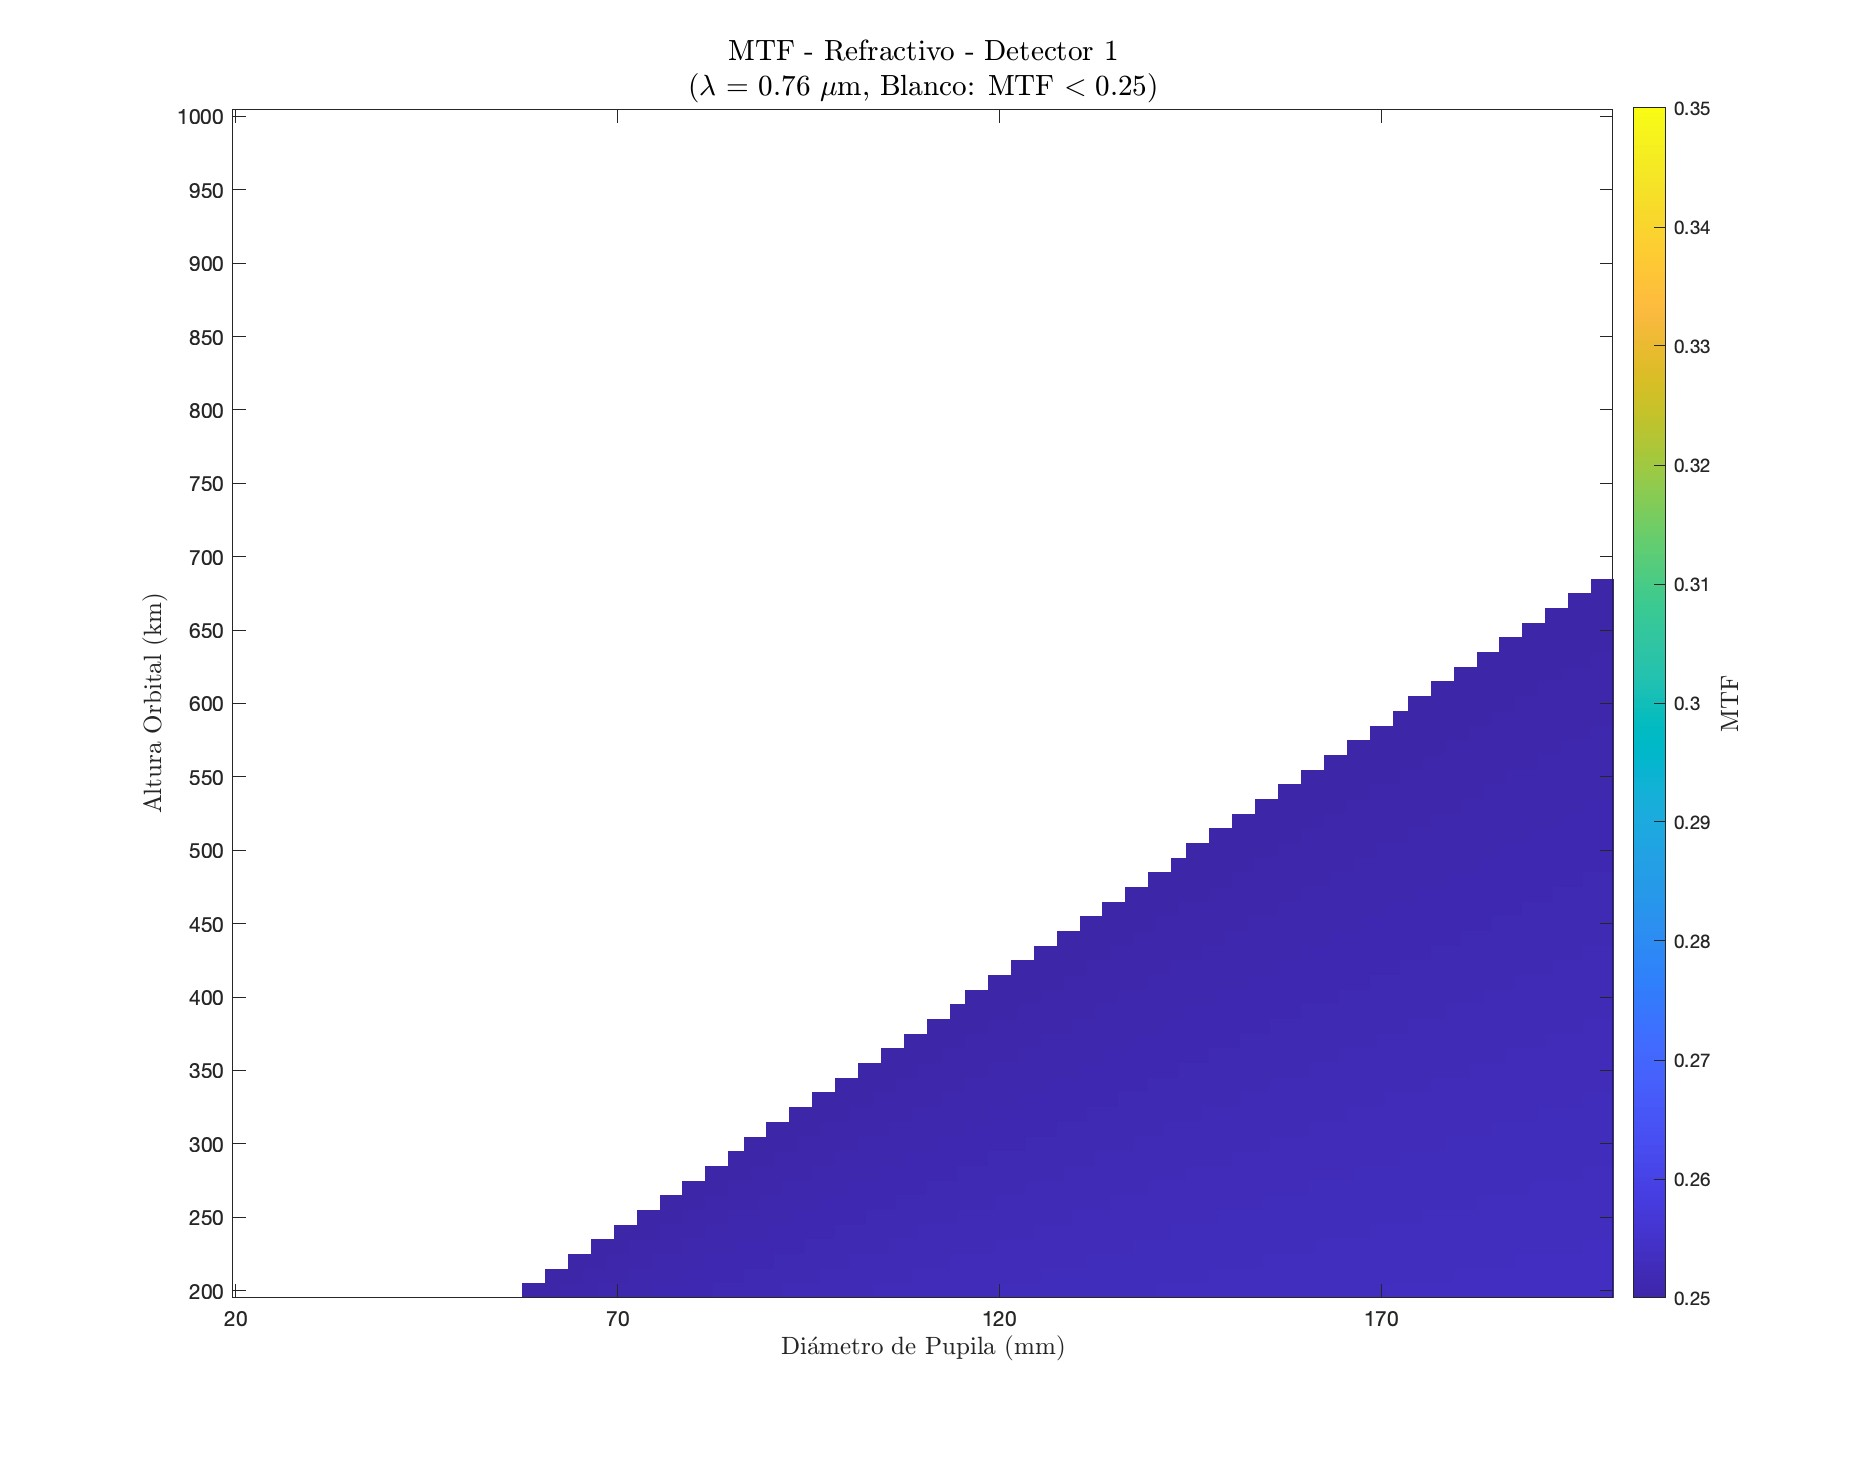
\includegraphics[width=0.48\linewidth]{4.Payload/MTF/MTF_Lambda3_Detector4_Telescopio1_heatmap.jpg} &
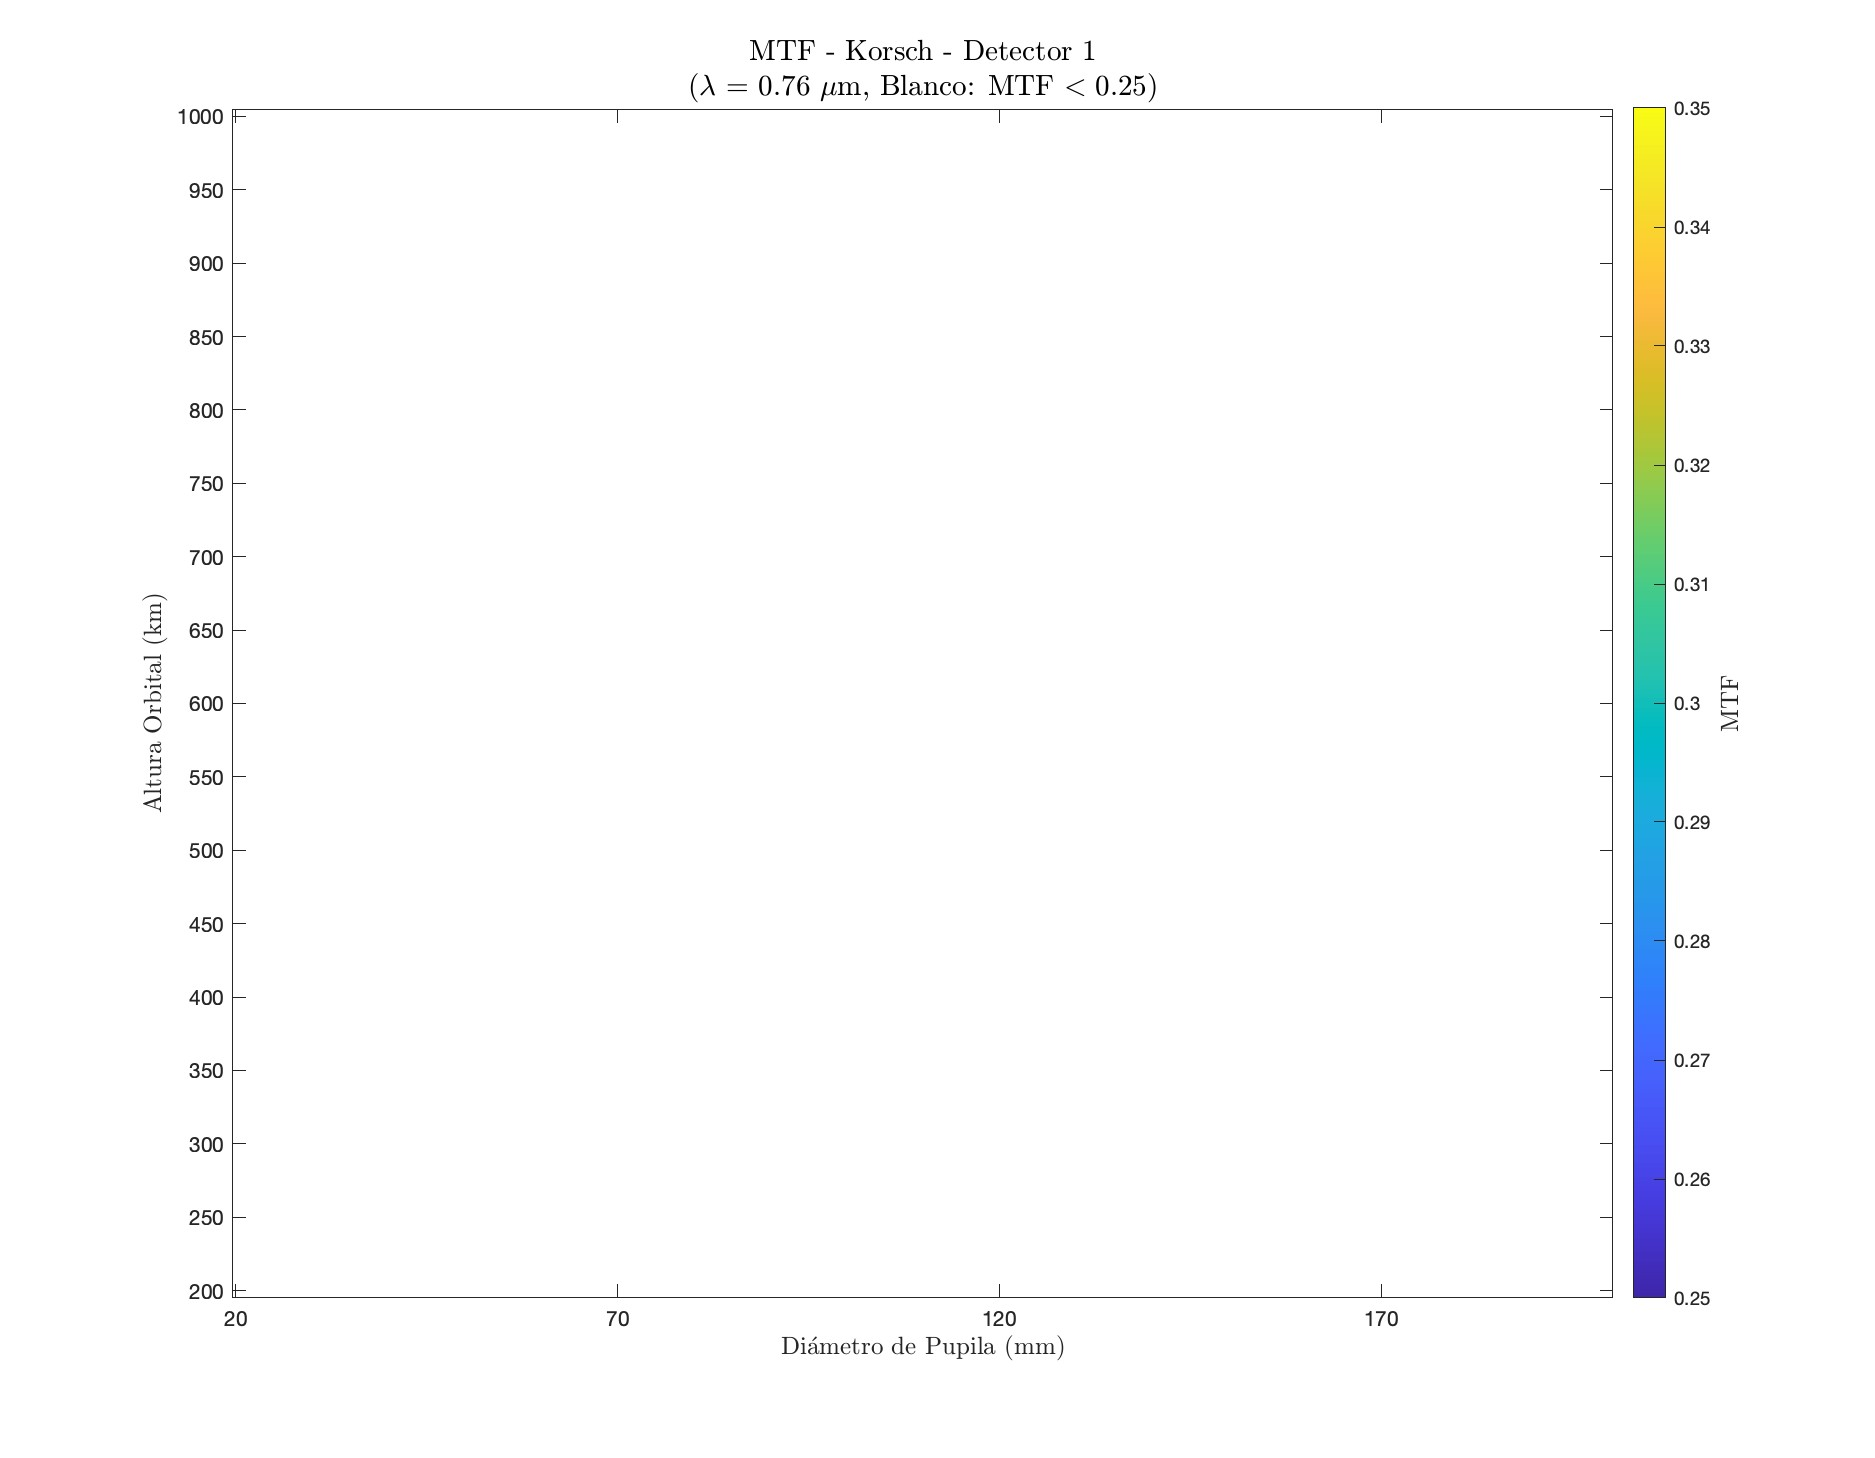
\includegraphics[width=0.48\linewidth]{4.Payload/MTF/MTF_Lambda3_Detector4_Telescopio2_heatmap.jpg} \\
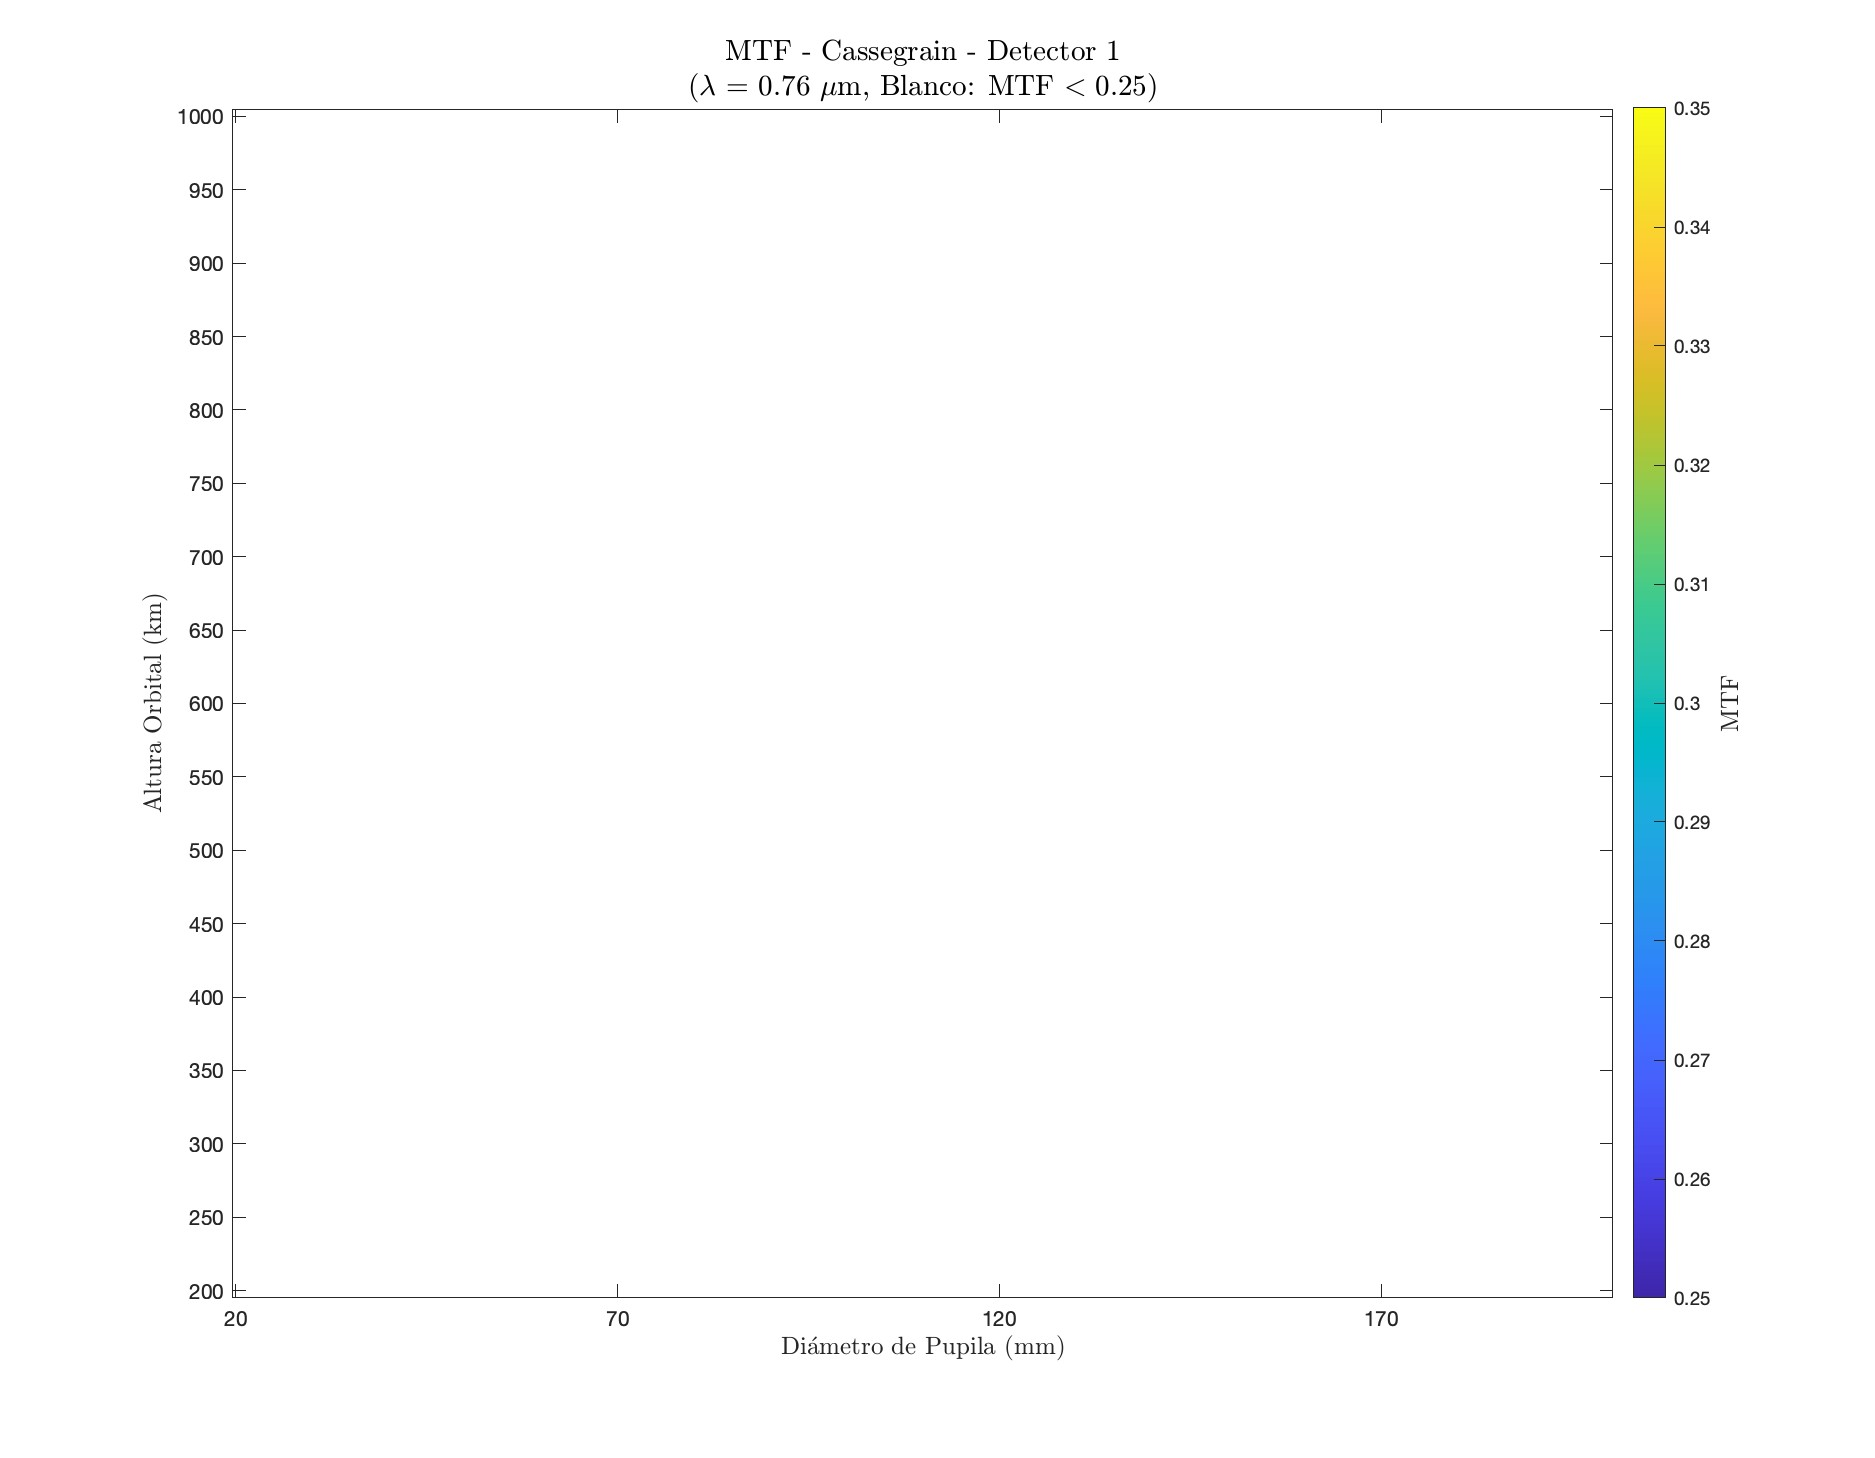
\includegraphics[width=0.48\linewidth]{4.Payload/MTF/MTF_Lambda3_Detector4_Telescopio3_heatmap.jpg} &
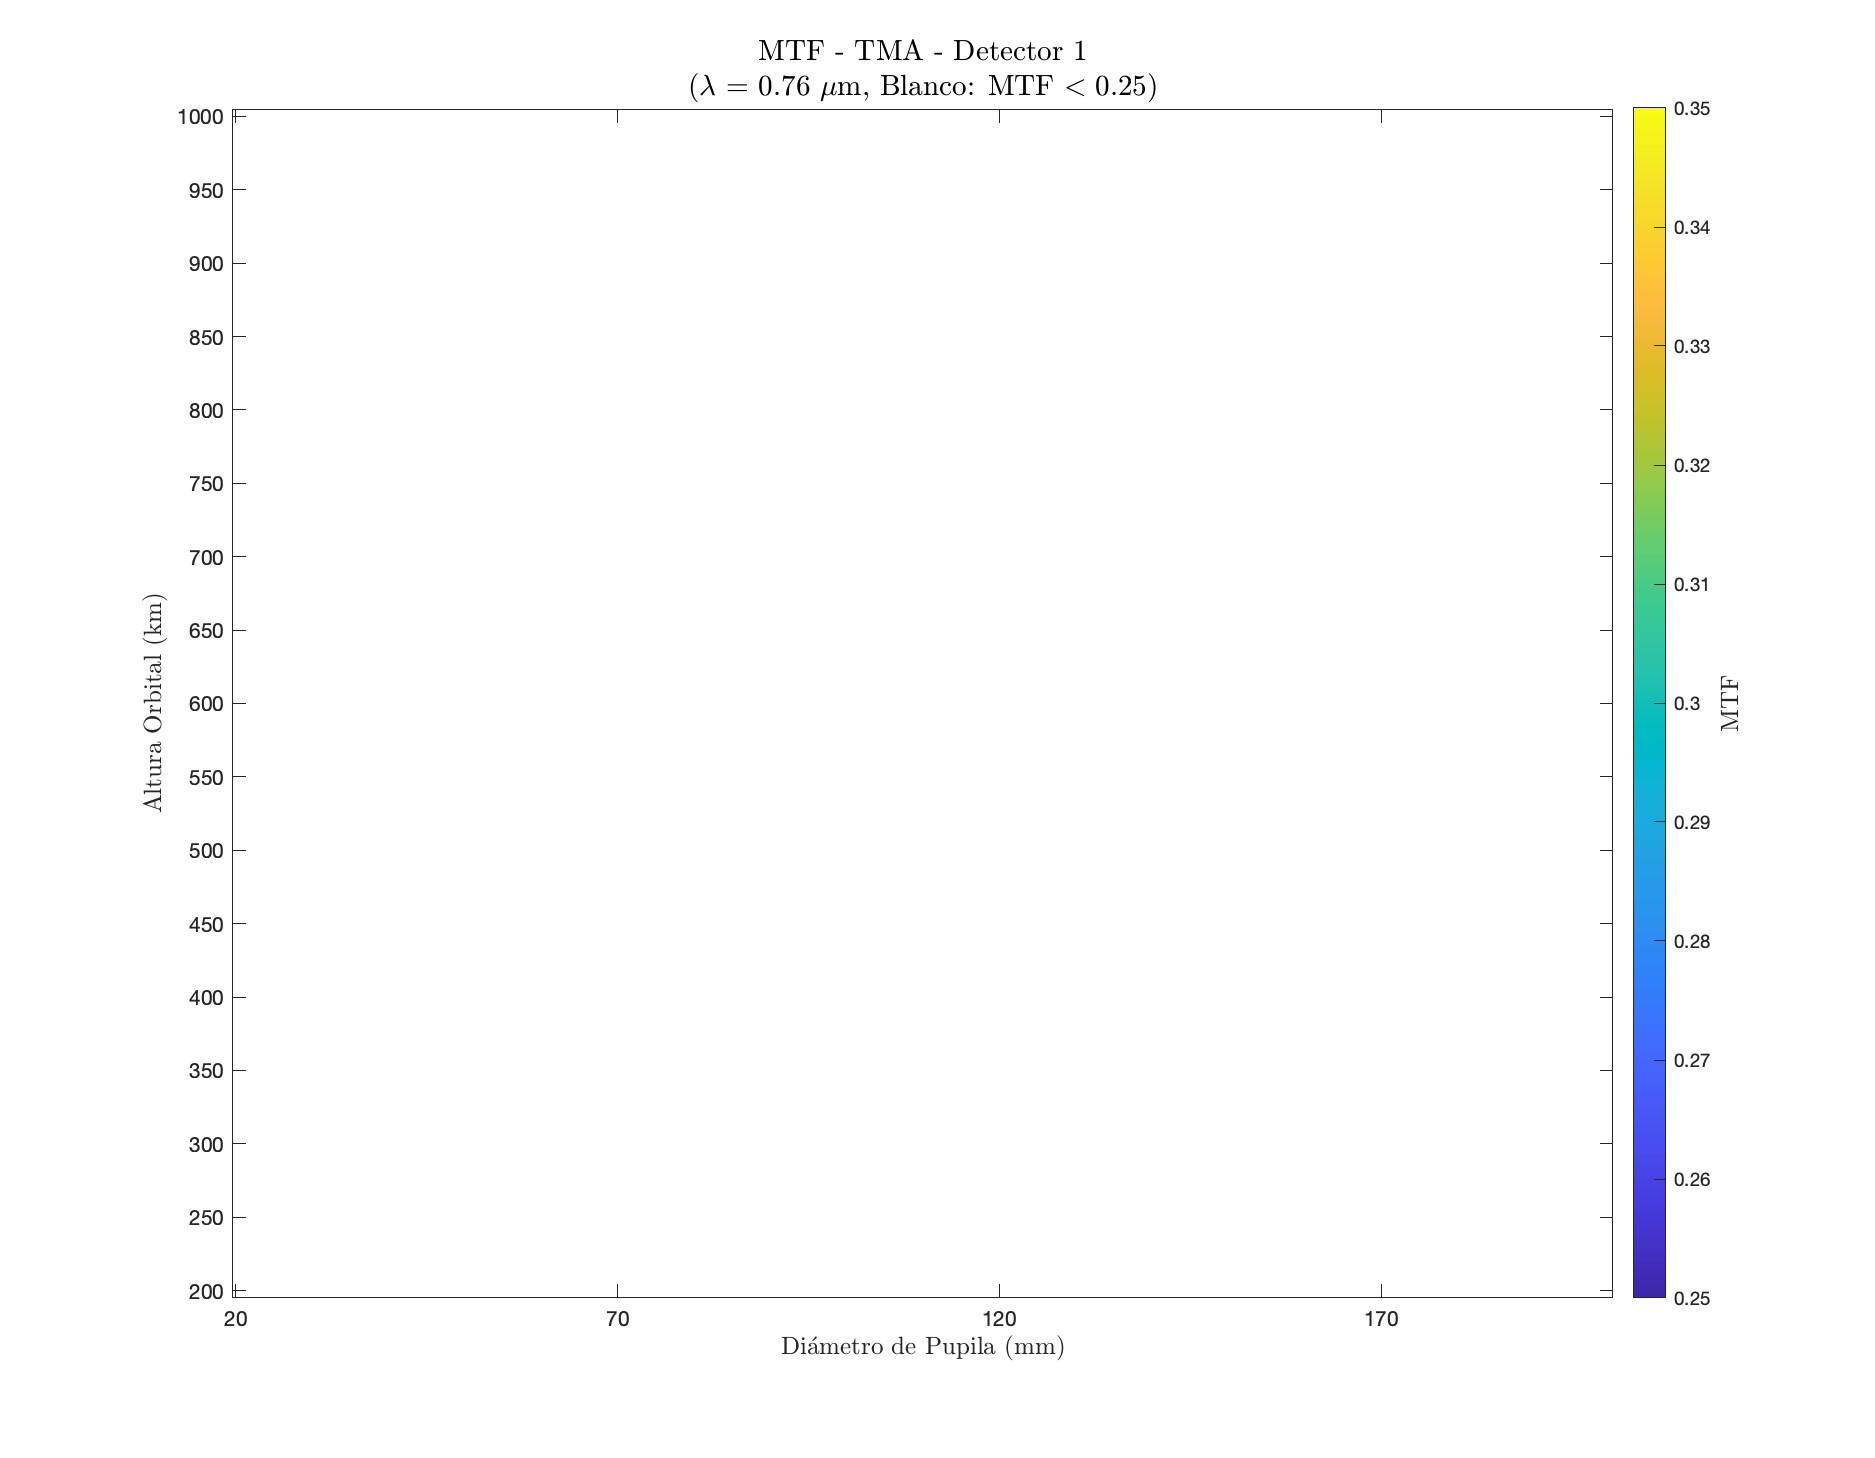
\includegraphics[width=0.48\linewidth]{4.Payload/MTF/MTF_Lambda3_Detector4_Telescopio4_heatmap.jpg} \\
\end{tabular}

\caption{Mapas de calor resultantes del calculo de MTF: Banda 0,76 \textmu m; Detector 1}
\end{figure}
\end{landscape}


%% DETECTOR 2
\begin{landscape}
\begin{figure}[p]
\centering
\setlength{\tabcolsep}{2pt}
\renewcommand{\arraystretch}{0}

\begin{tabular}{cc}
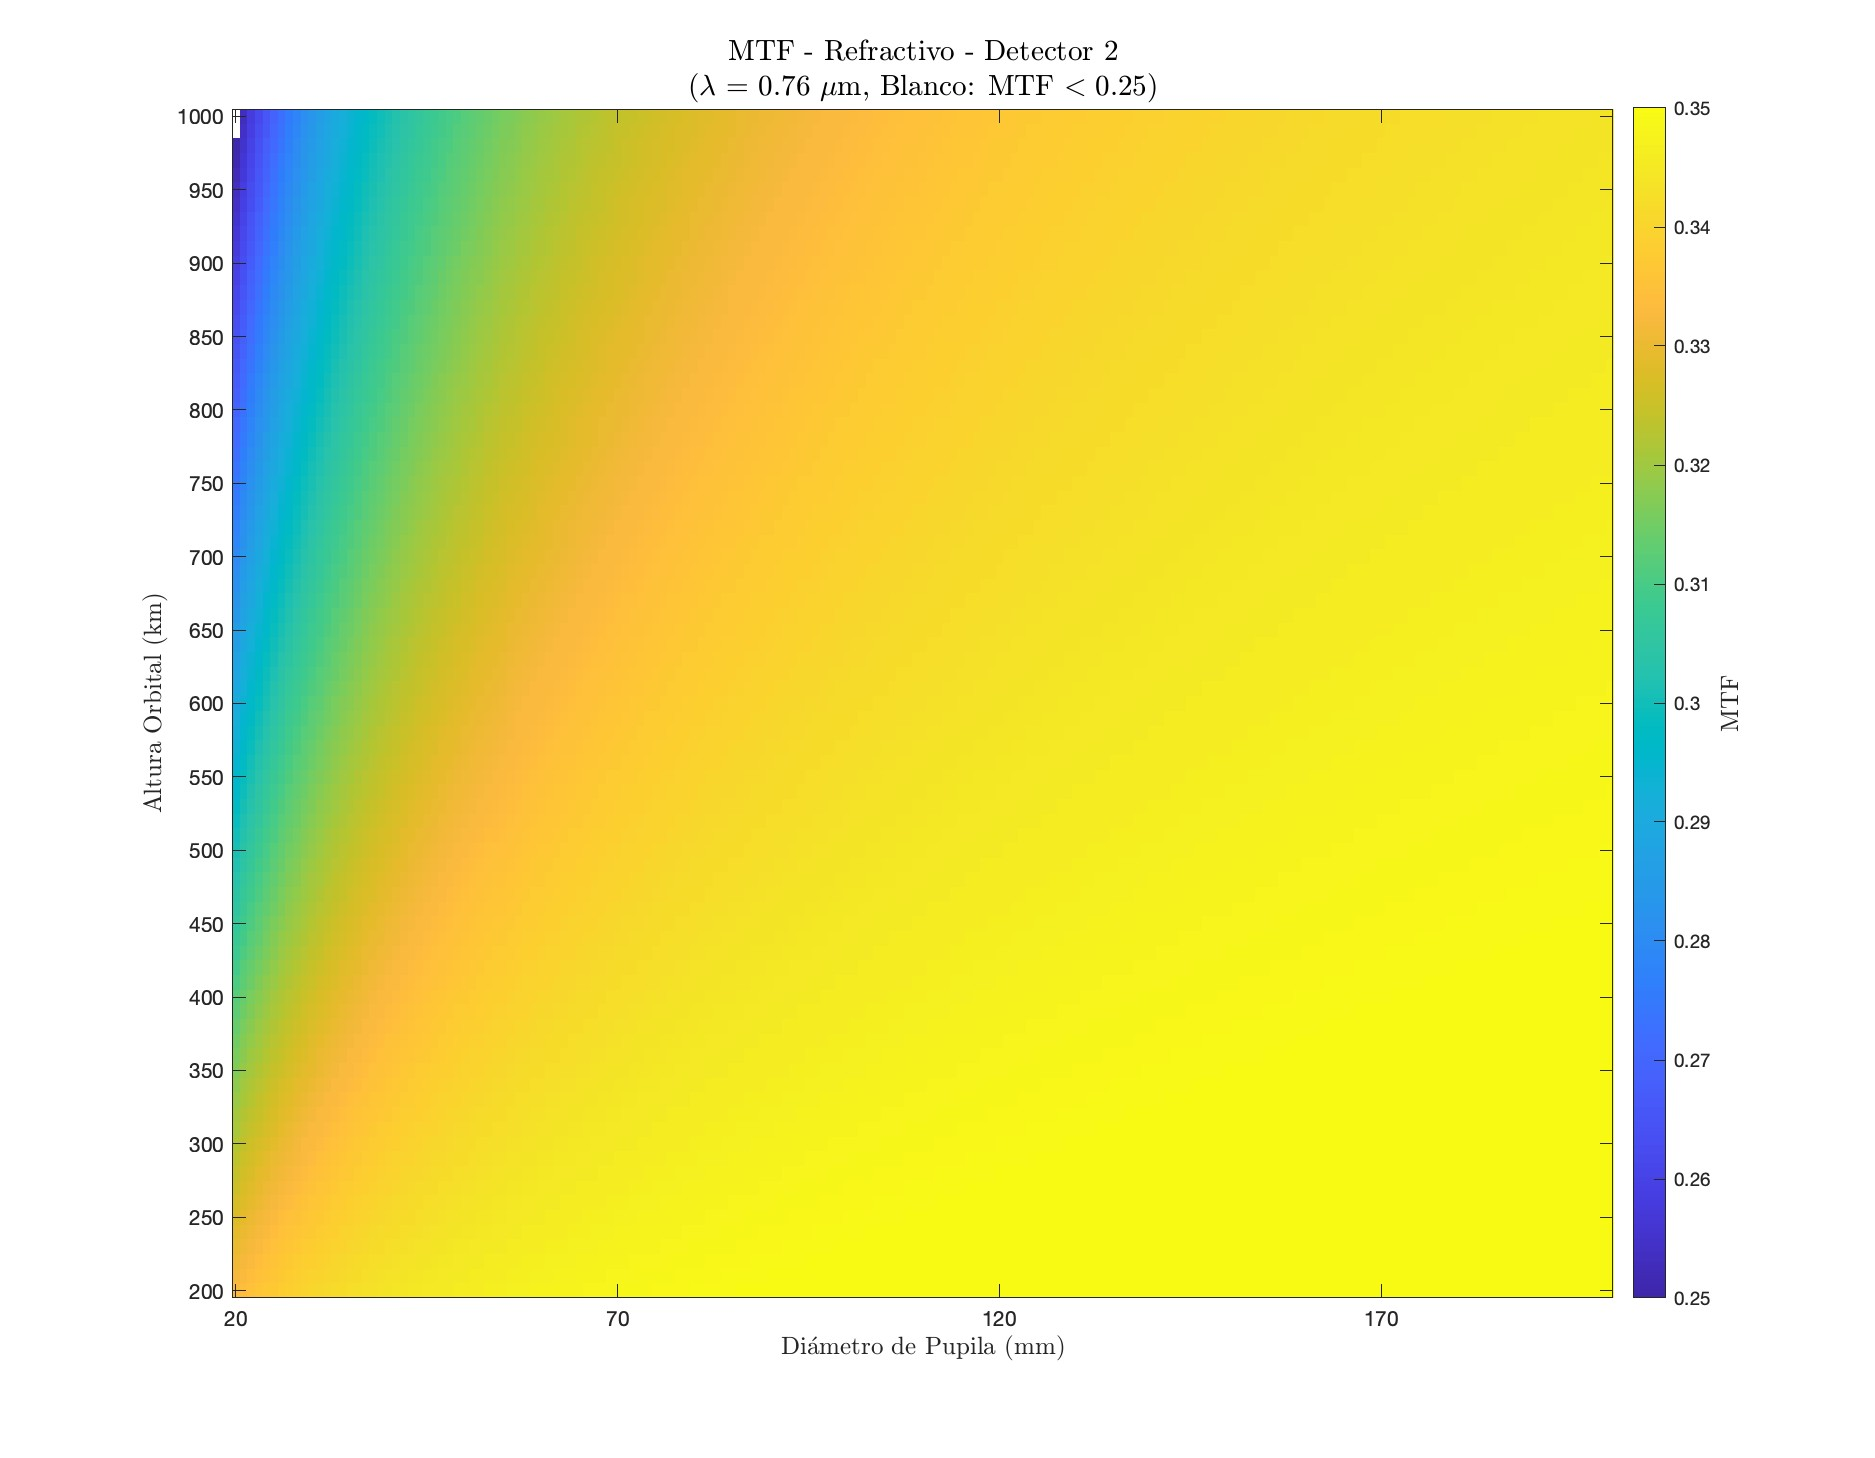
\includegraphics[width=0.48\linewidth]{4.Payload/MTF/MTF_Lambda3_Detector5_Telescopio1_heatmap.jpg} &
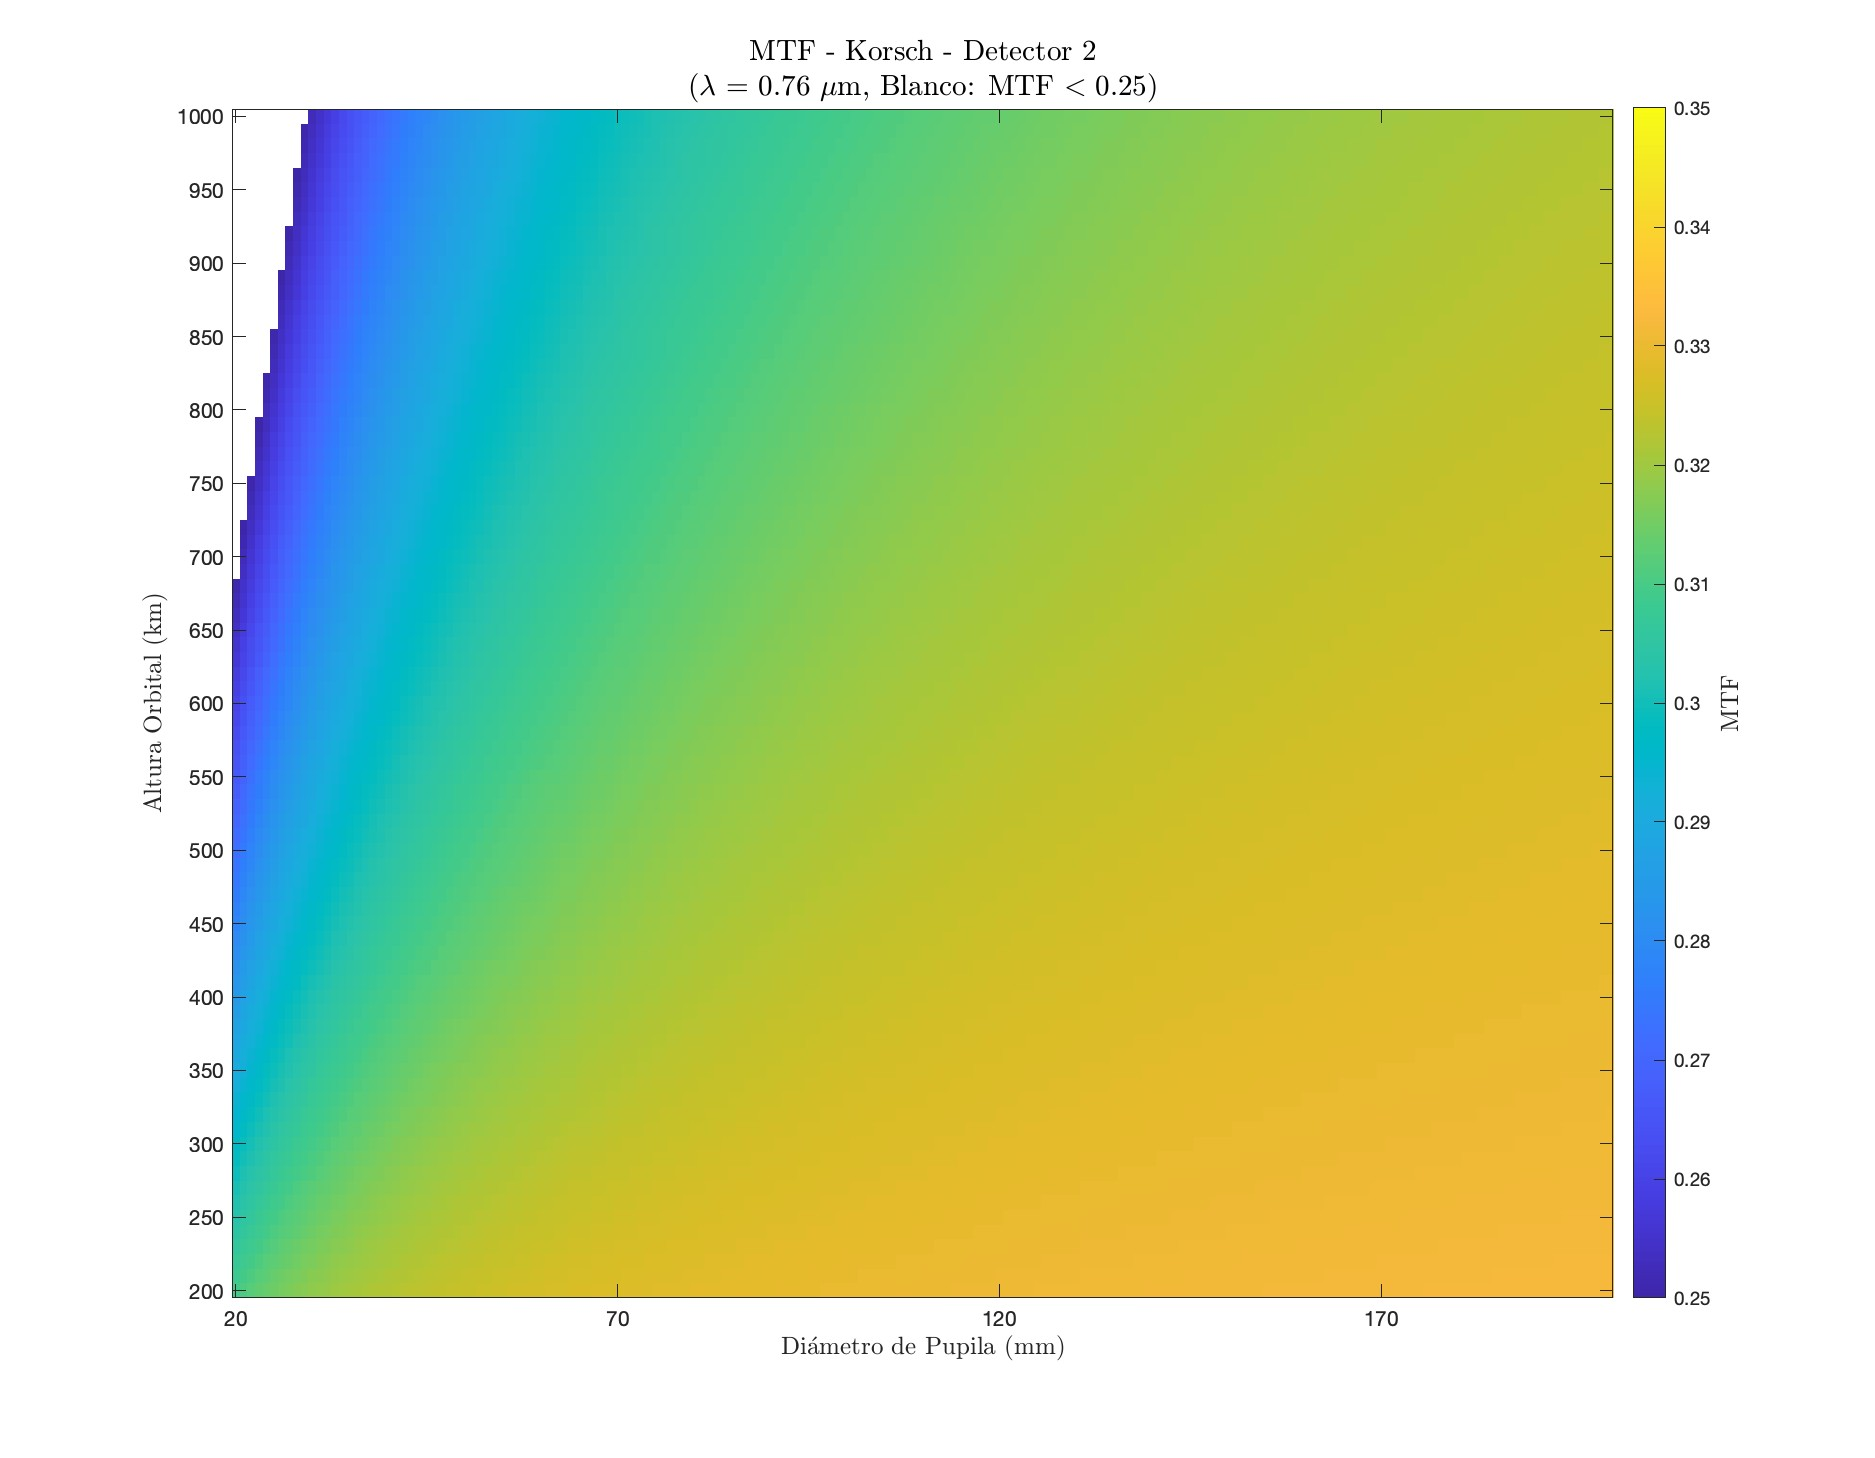
\includegraphics[width=0.48\linewidth]{4.Payload/MTF/MTF_Lambda3_Detector5_Telescopio2_heatmap.jpg} \\
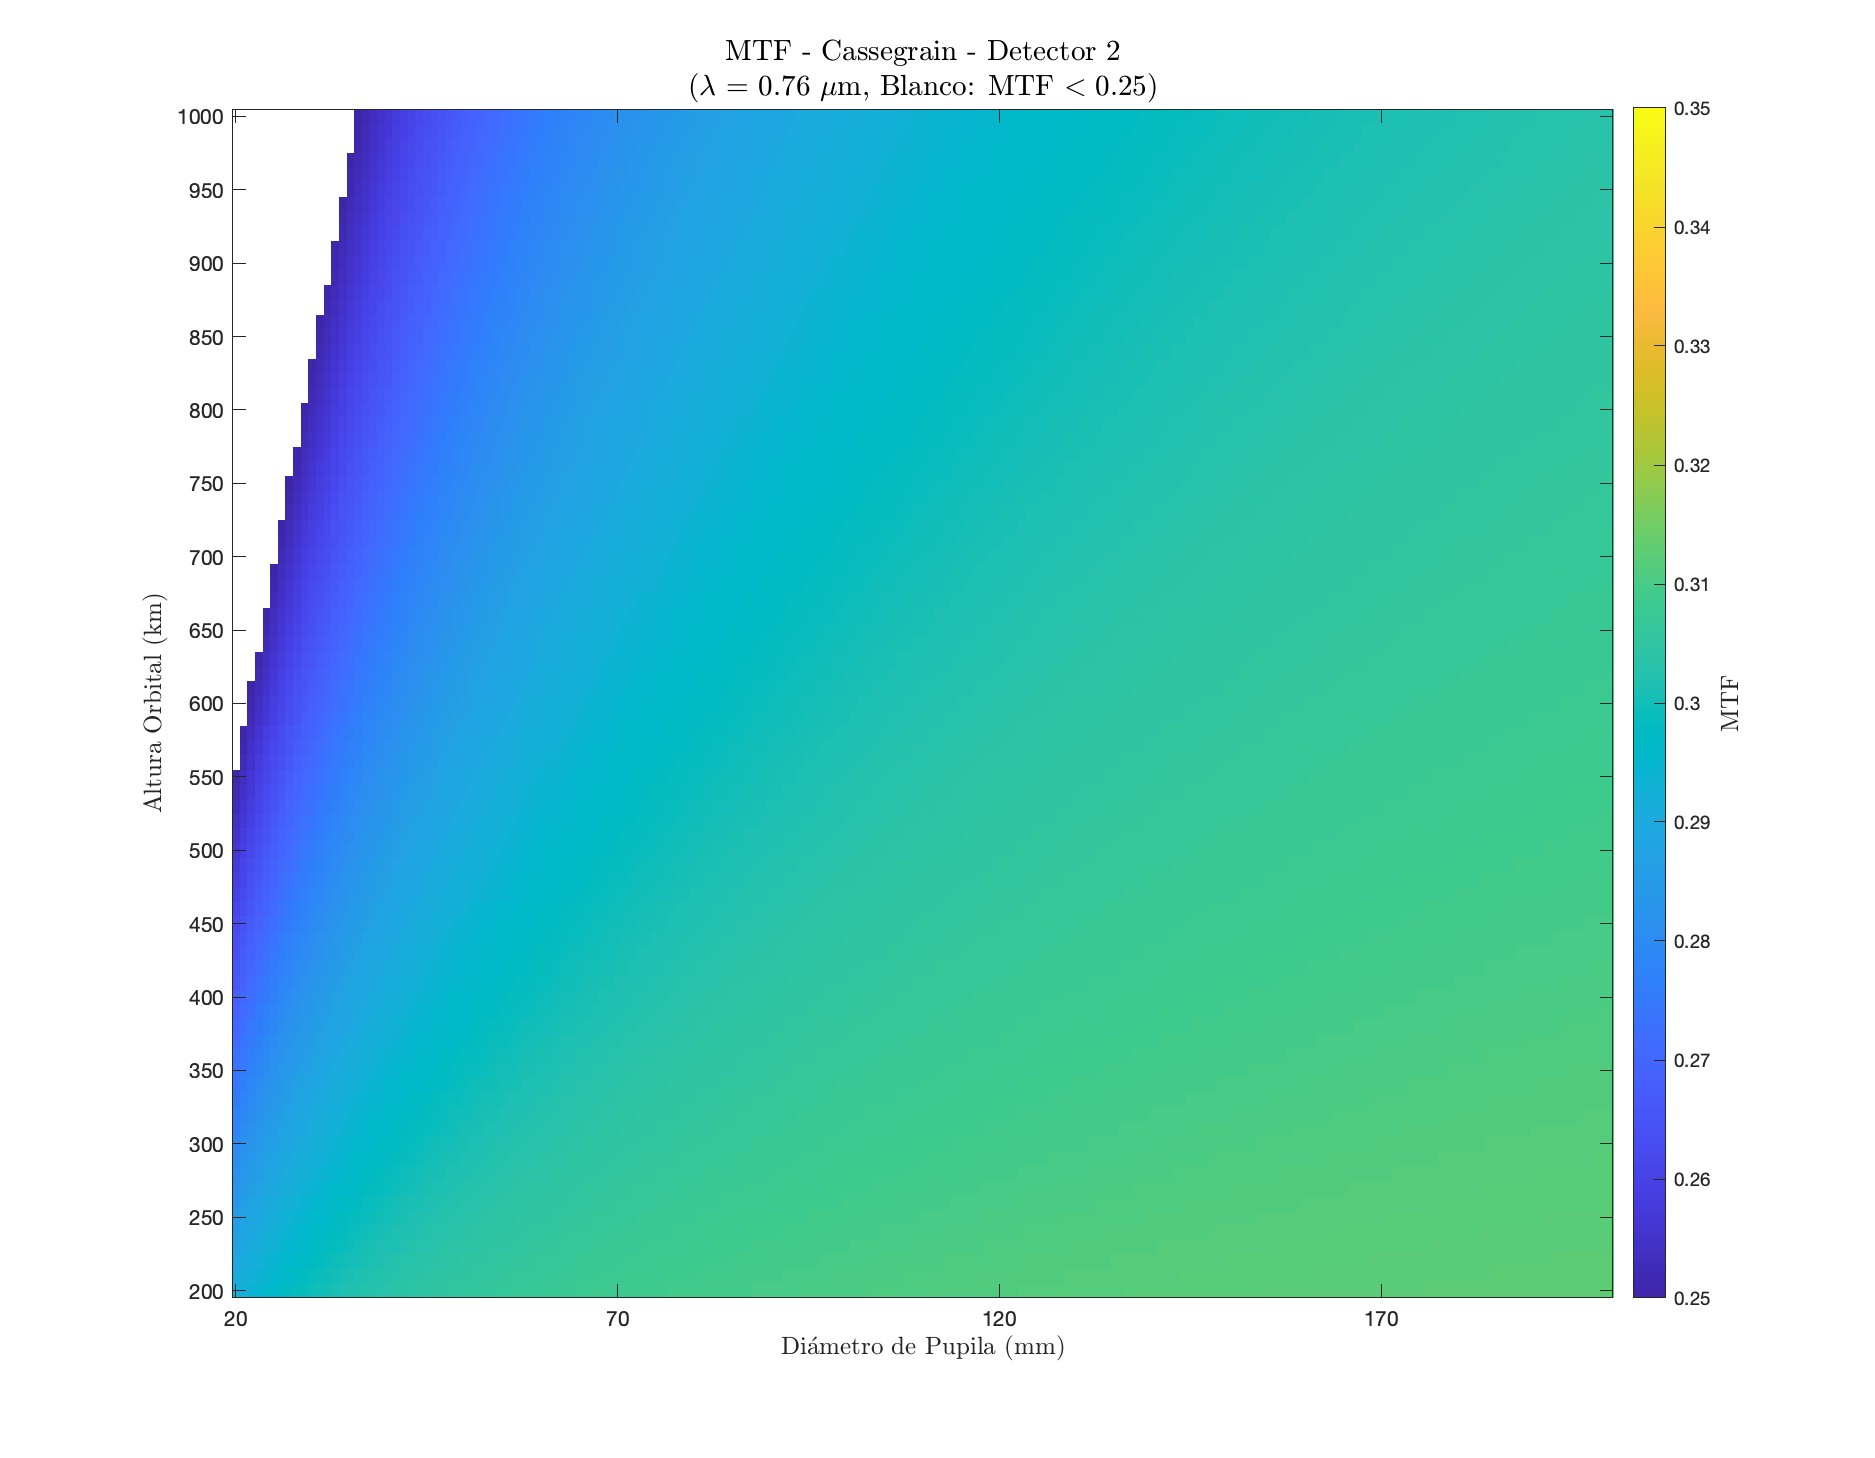
\includegraphics[width=0.48\linewidth]{4.Payload/MTF/MTF_Lambda3_Detector5_Telescopio3_heatmap.jpg} &
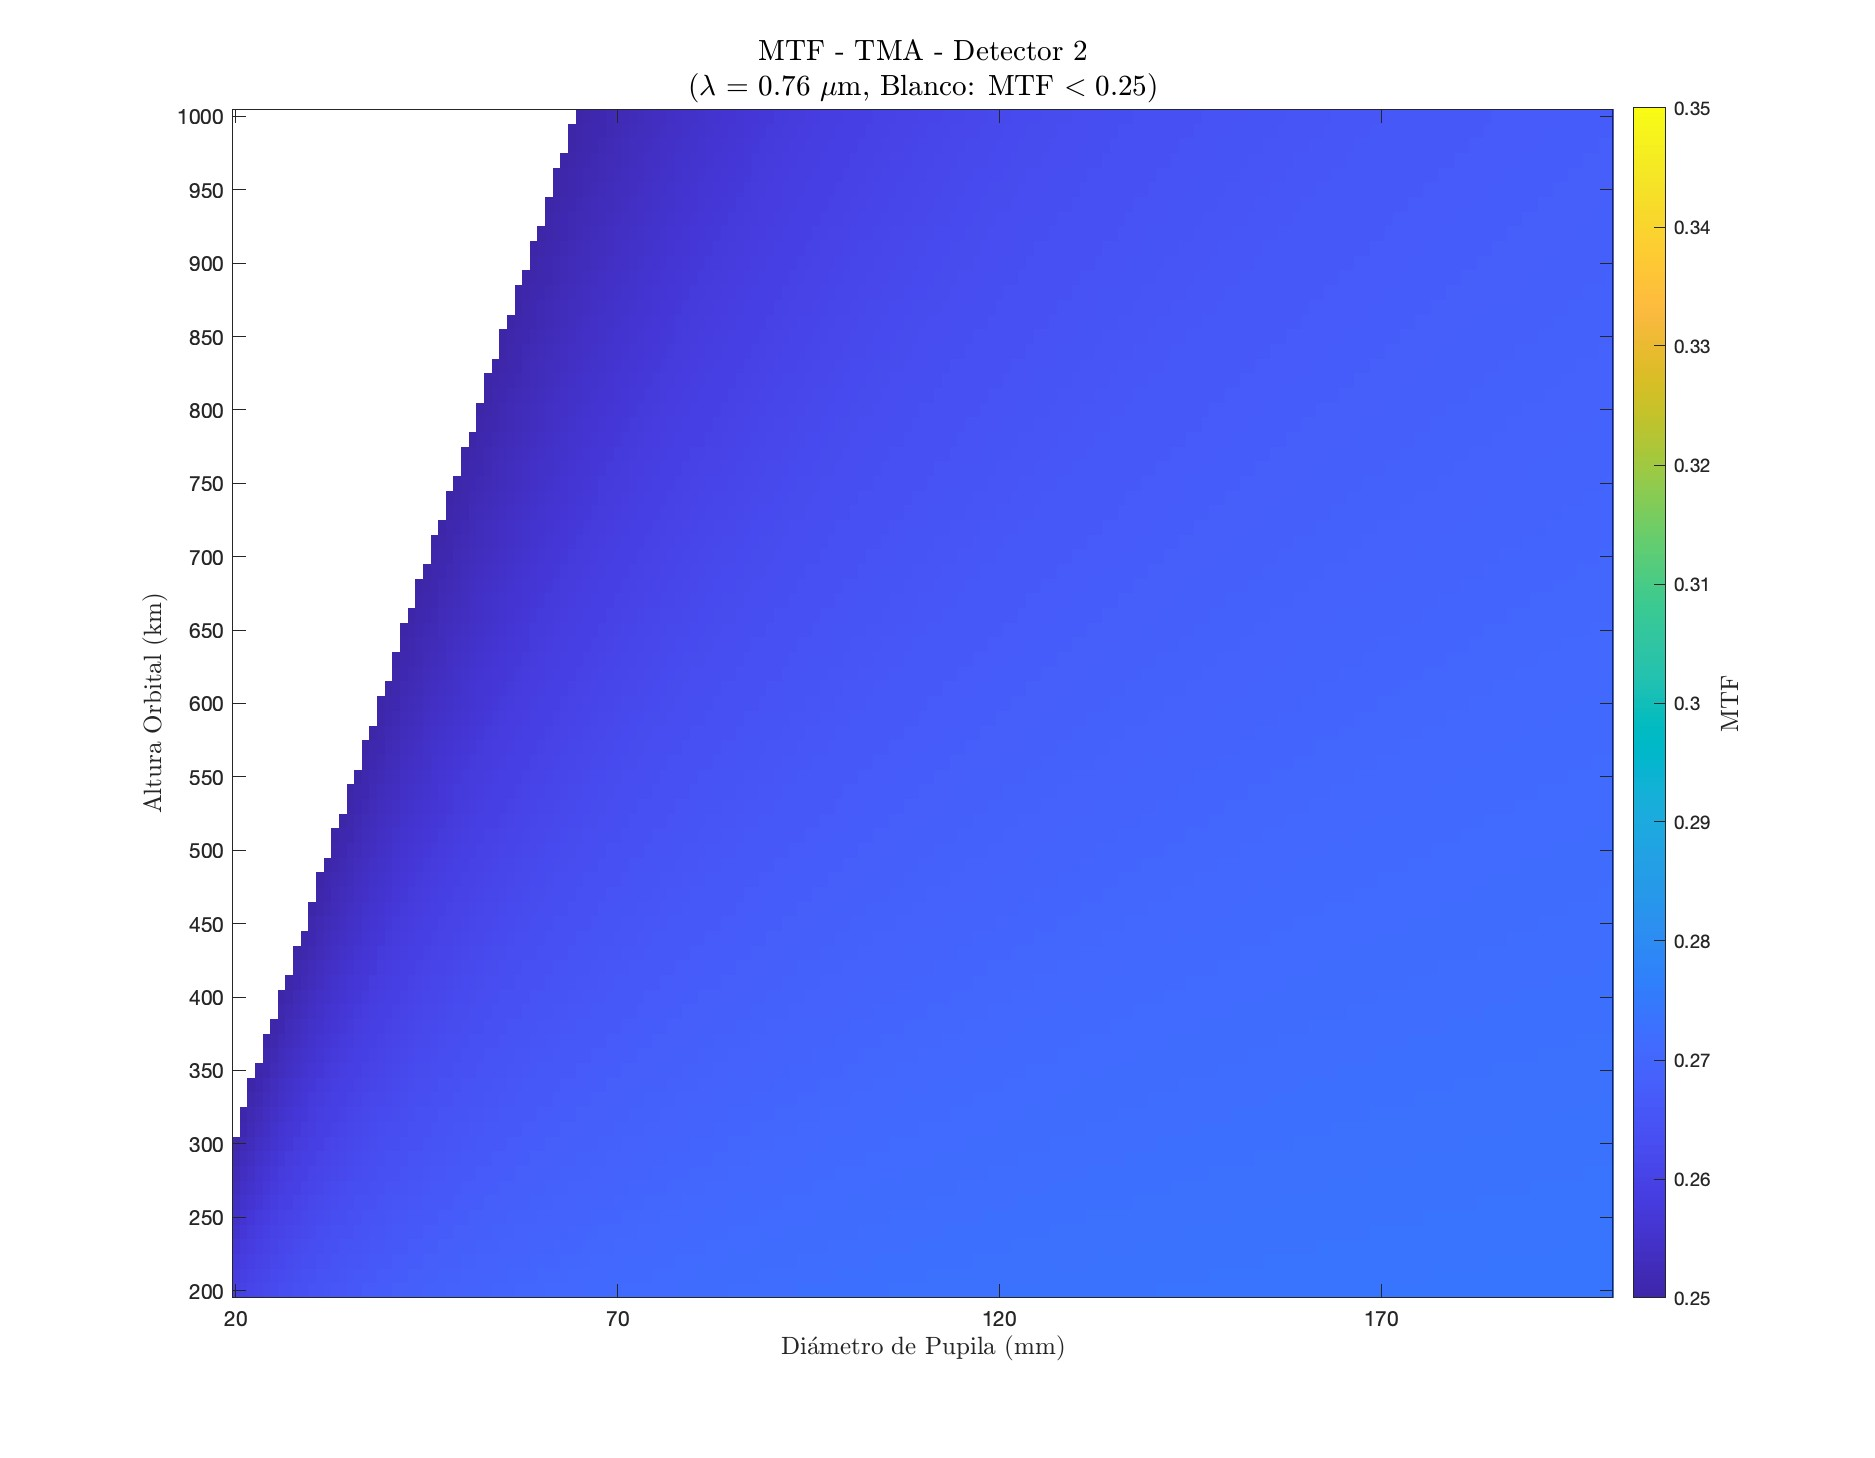
\includegraphics[width=0.48\linewidth]{4.Payload/MTF/MTF_Lambda3_Detector5_Telescopio4_heatmap.jpg} \\
\end{tabular}
\caption{Mapas de calor resultantes del calculo de MTF: Banda 0,76 \textmu m; Detector 2}
\end{figure}
\end{landscape}


%% DETECTOR 3
\begin{landscape}
\begin{figure}[p]
\centering
\setlength{\tabcolsep}{2pt}
\renewcommand{\arraystretch}{0}

\begin{tabular}{cc}
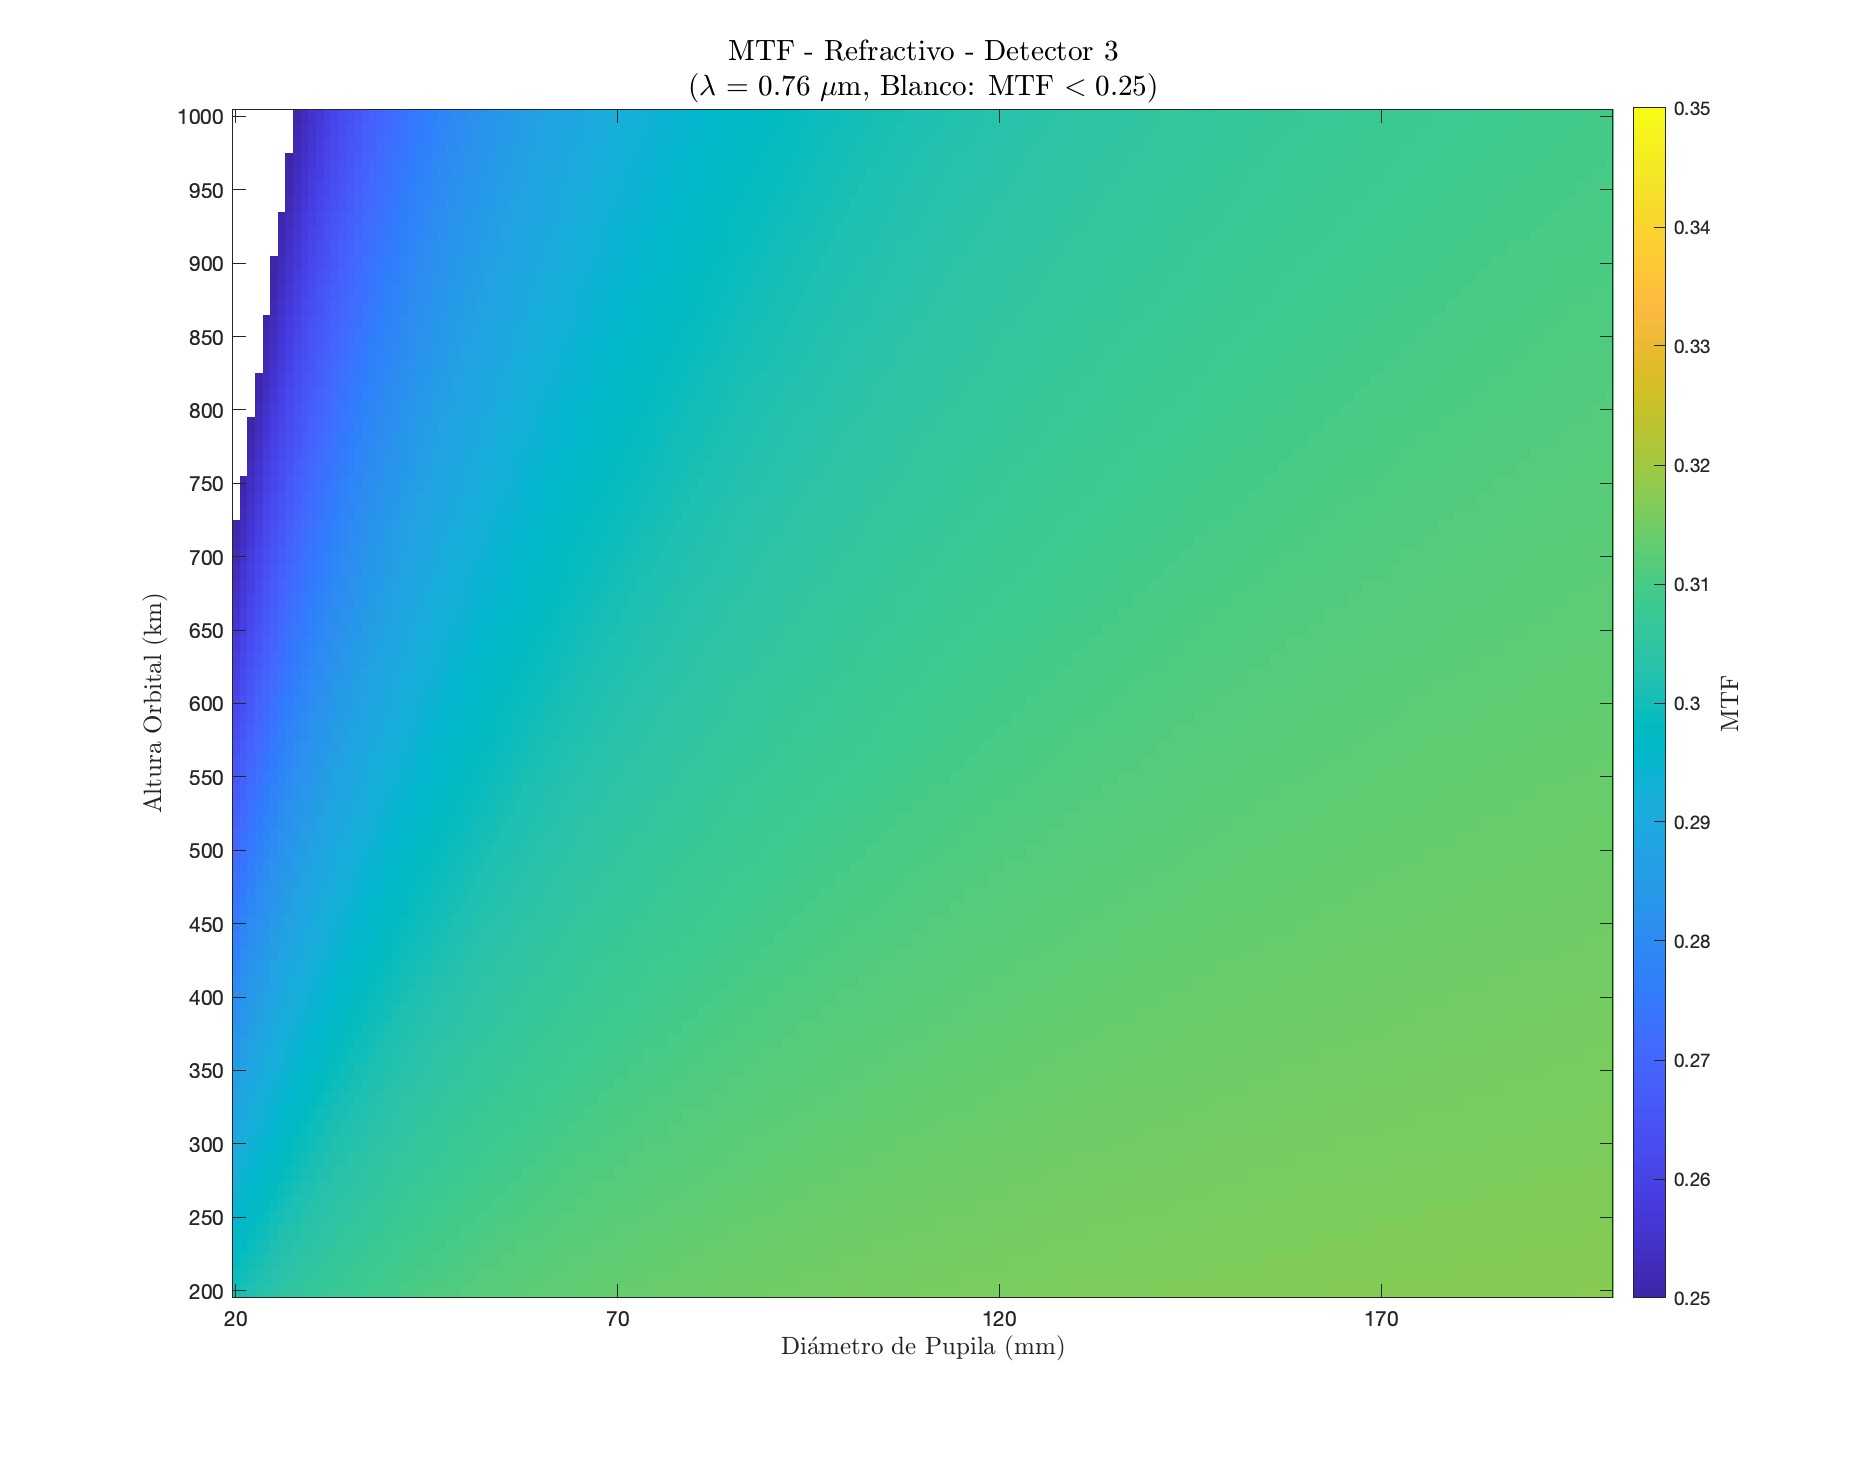
\includegraphics[width=0.48\linewidth]{4.Payload/MTF/MTF_Lambda3_Detector6_Telescopio1_heatmap.jpg} &
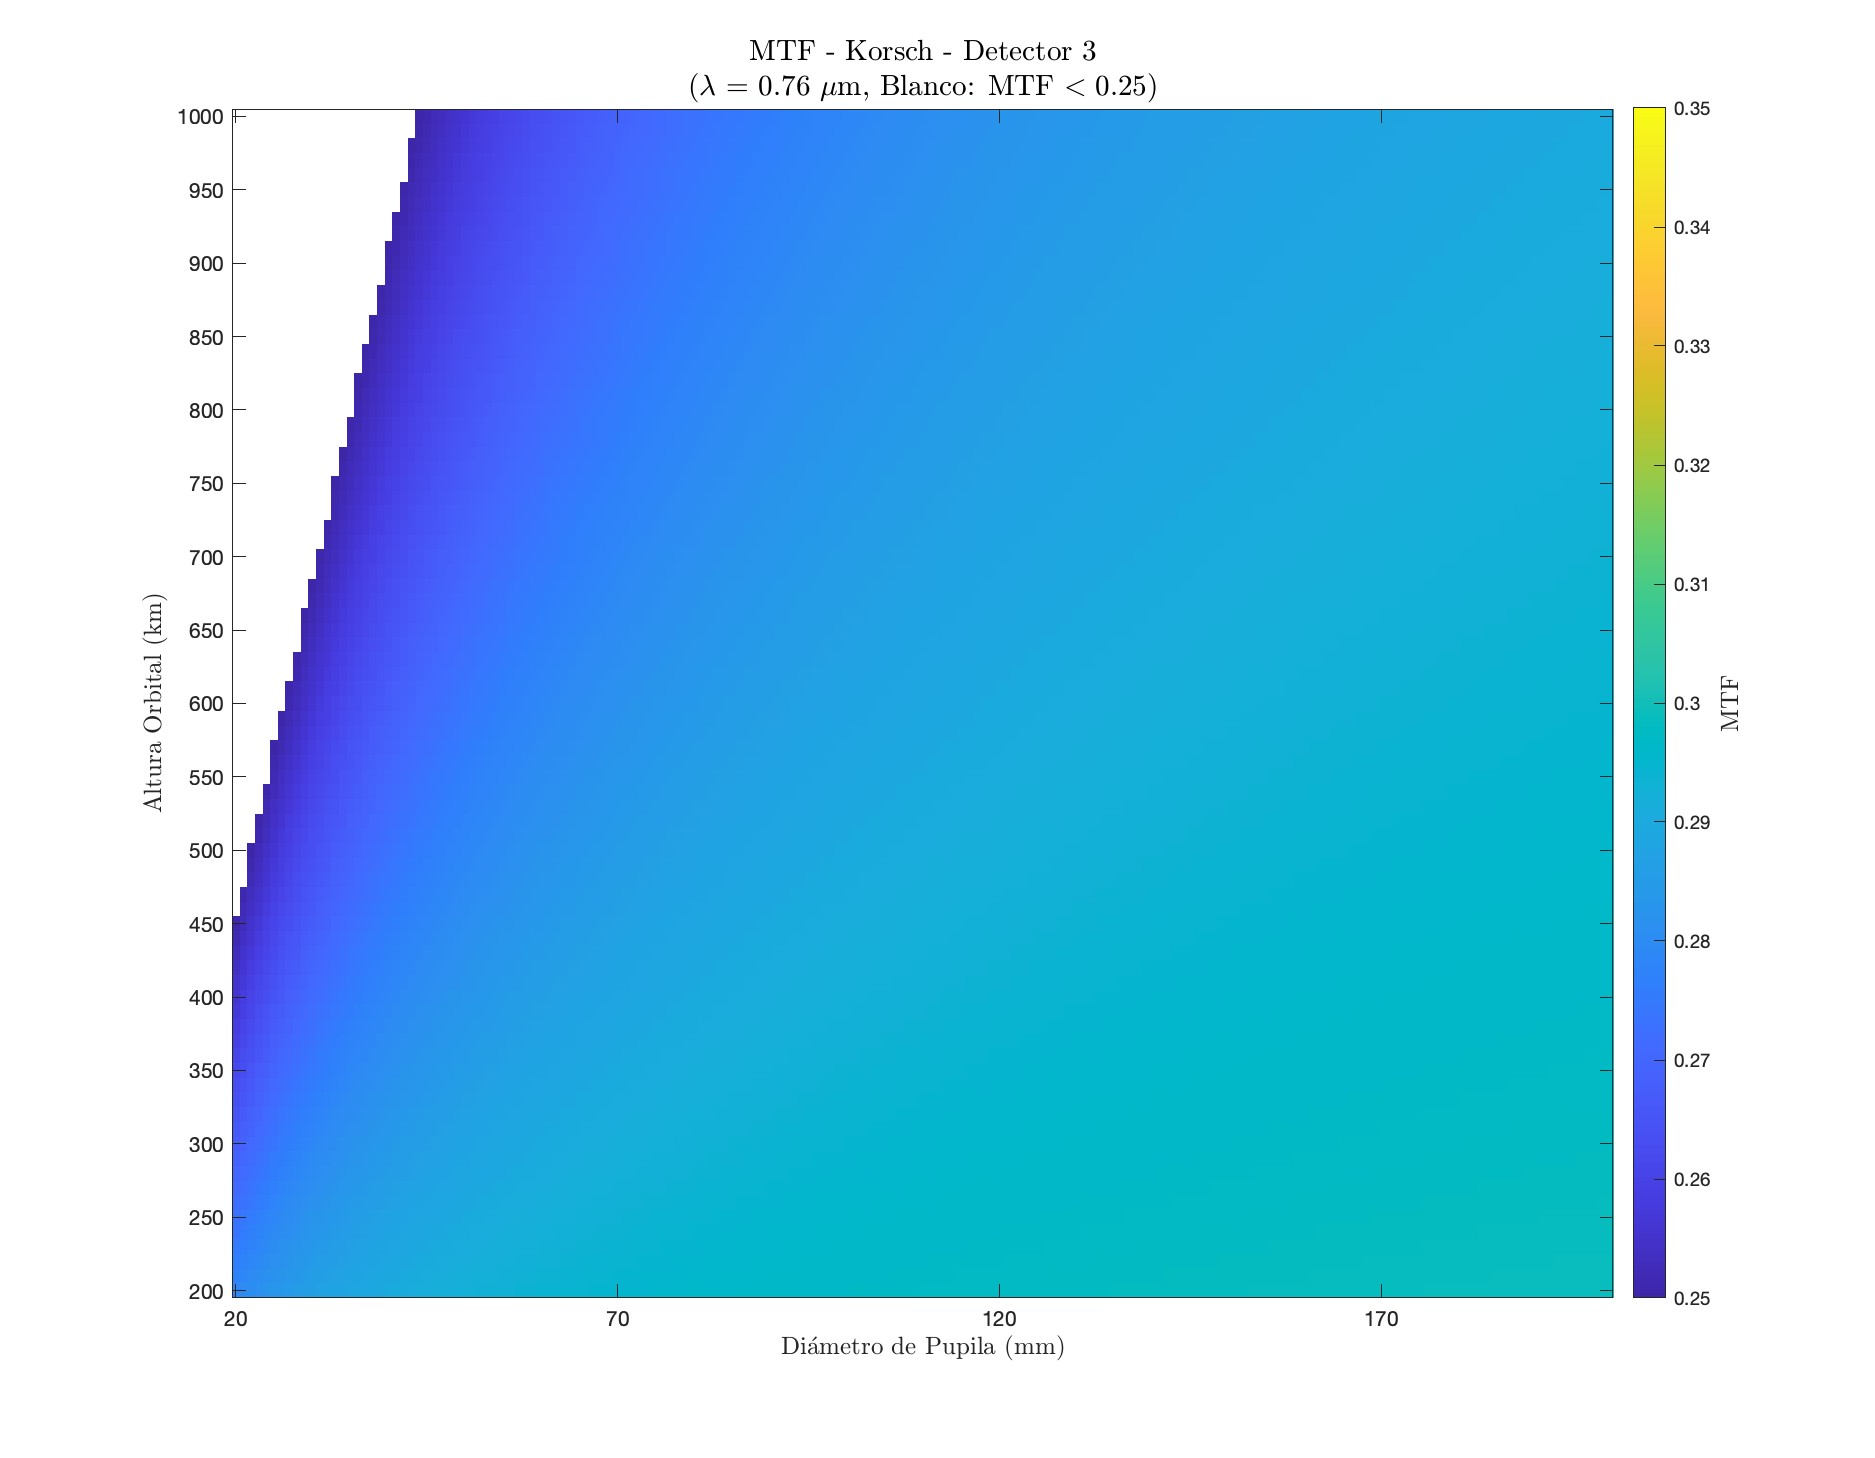
\includegraphics[width=0.48\linewidth]{4.Payload/MTF/MTF_Lambda3_Detector6_Telescopio2_heatmap.jpg} \\
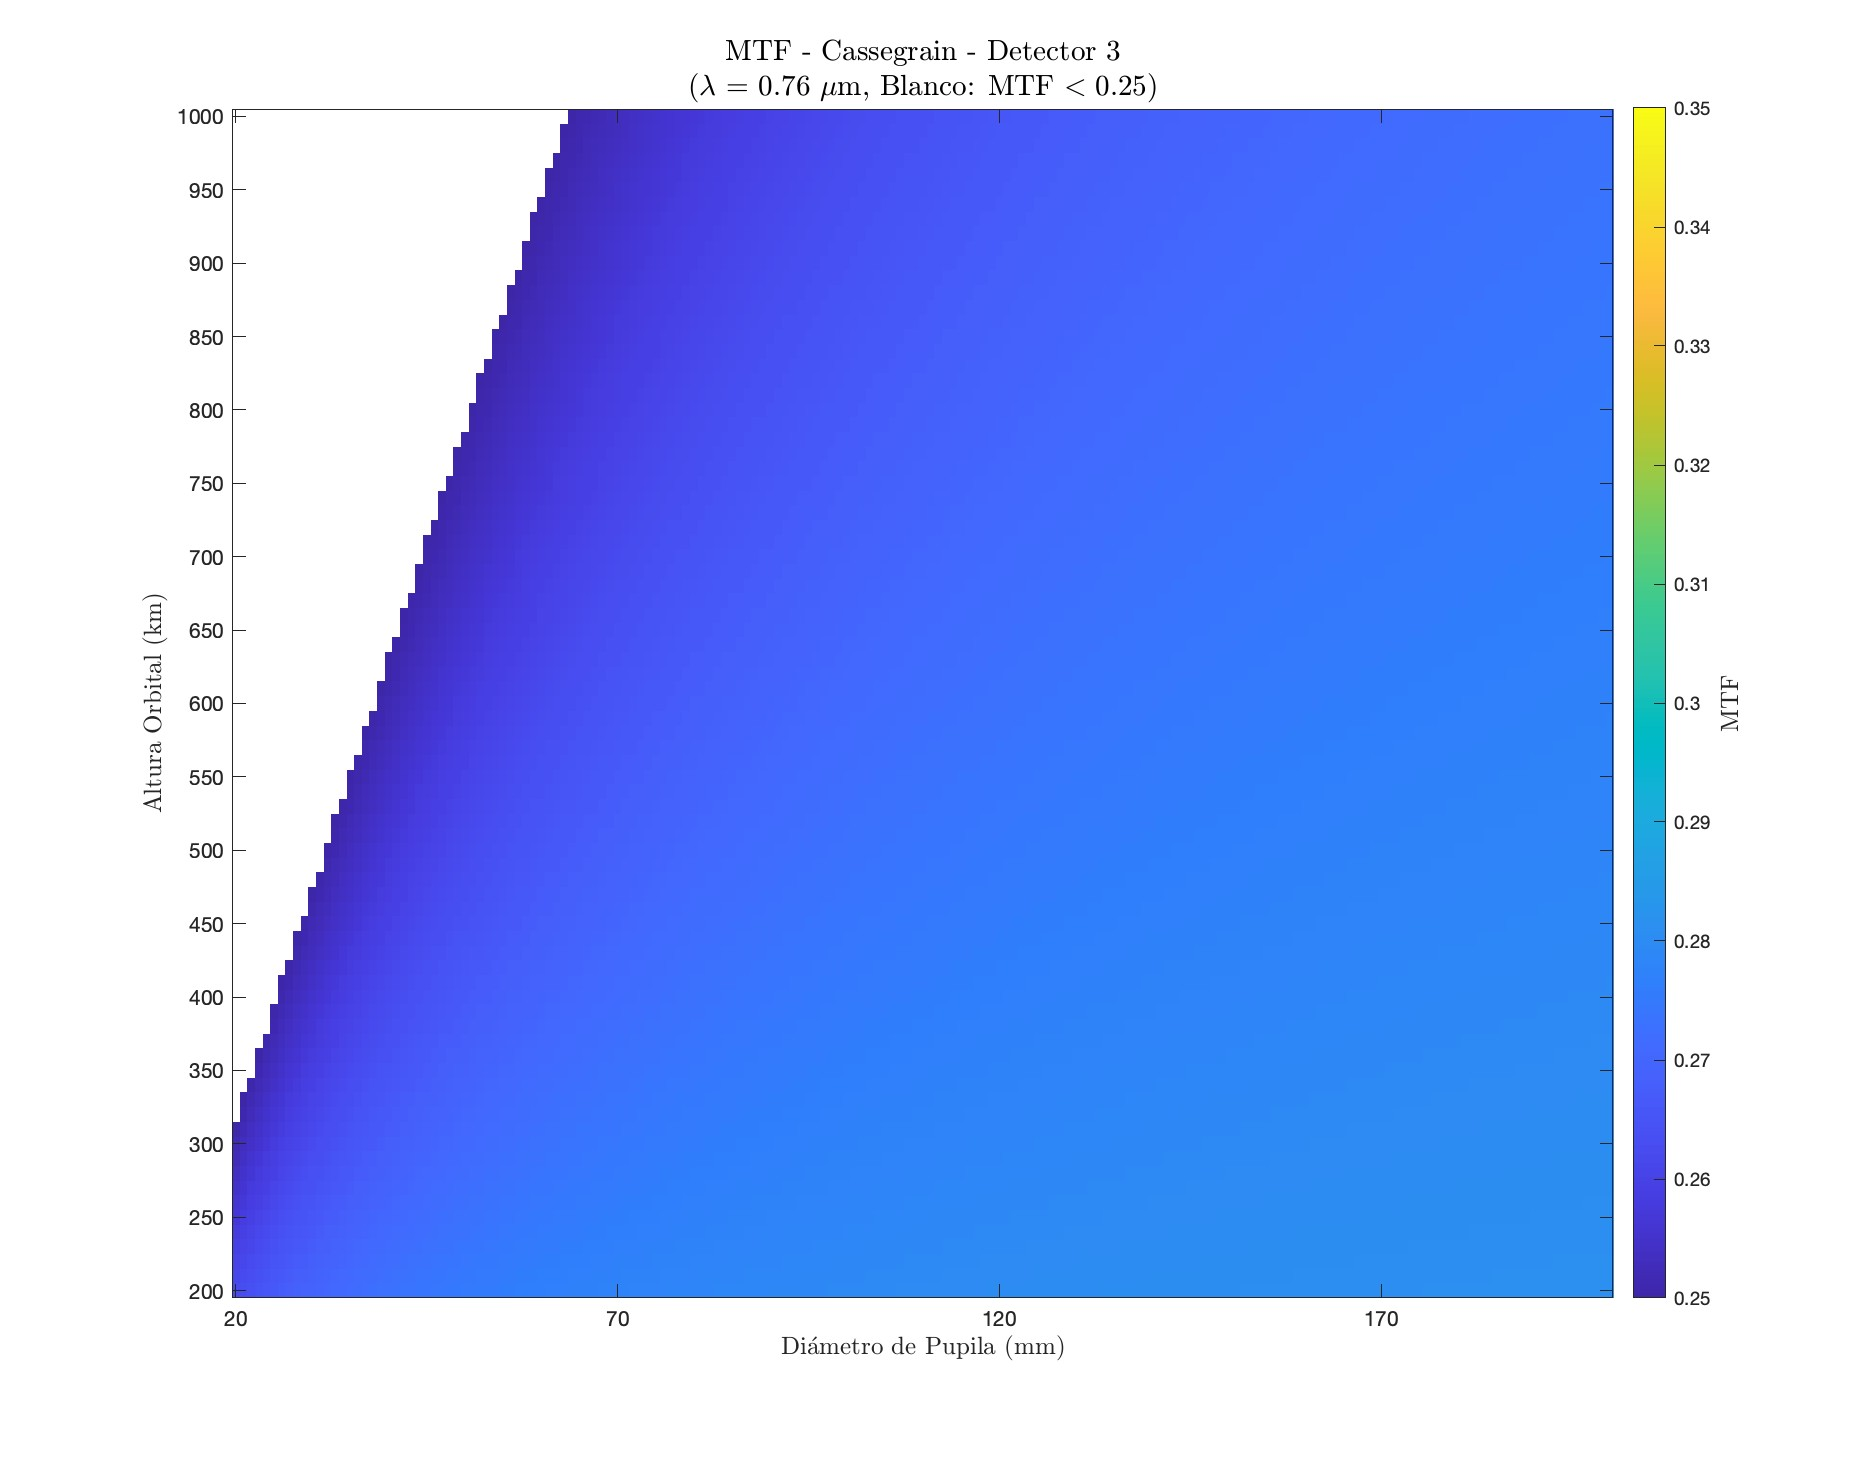
\includegraphics[width=0.48\linewidth]{4.Payload/MTF/MTF_Lambda3_Detector6_Telescopio3_heatmap.jpg} &
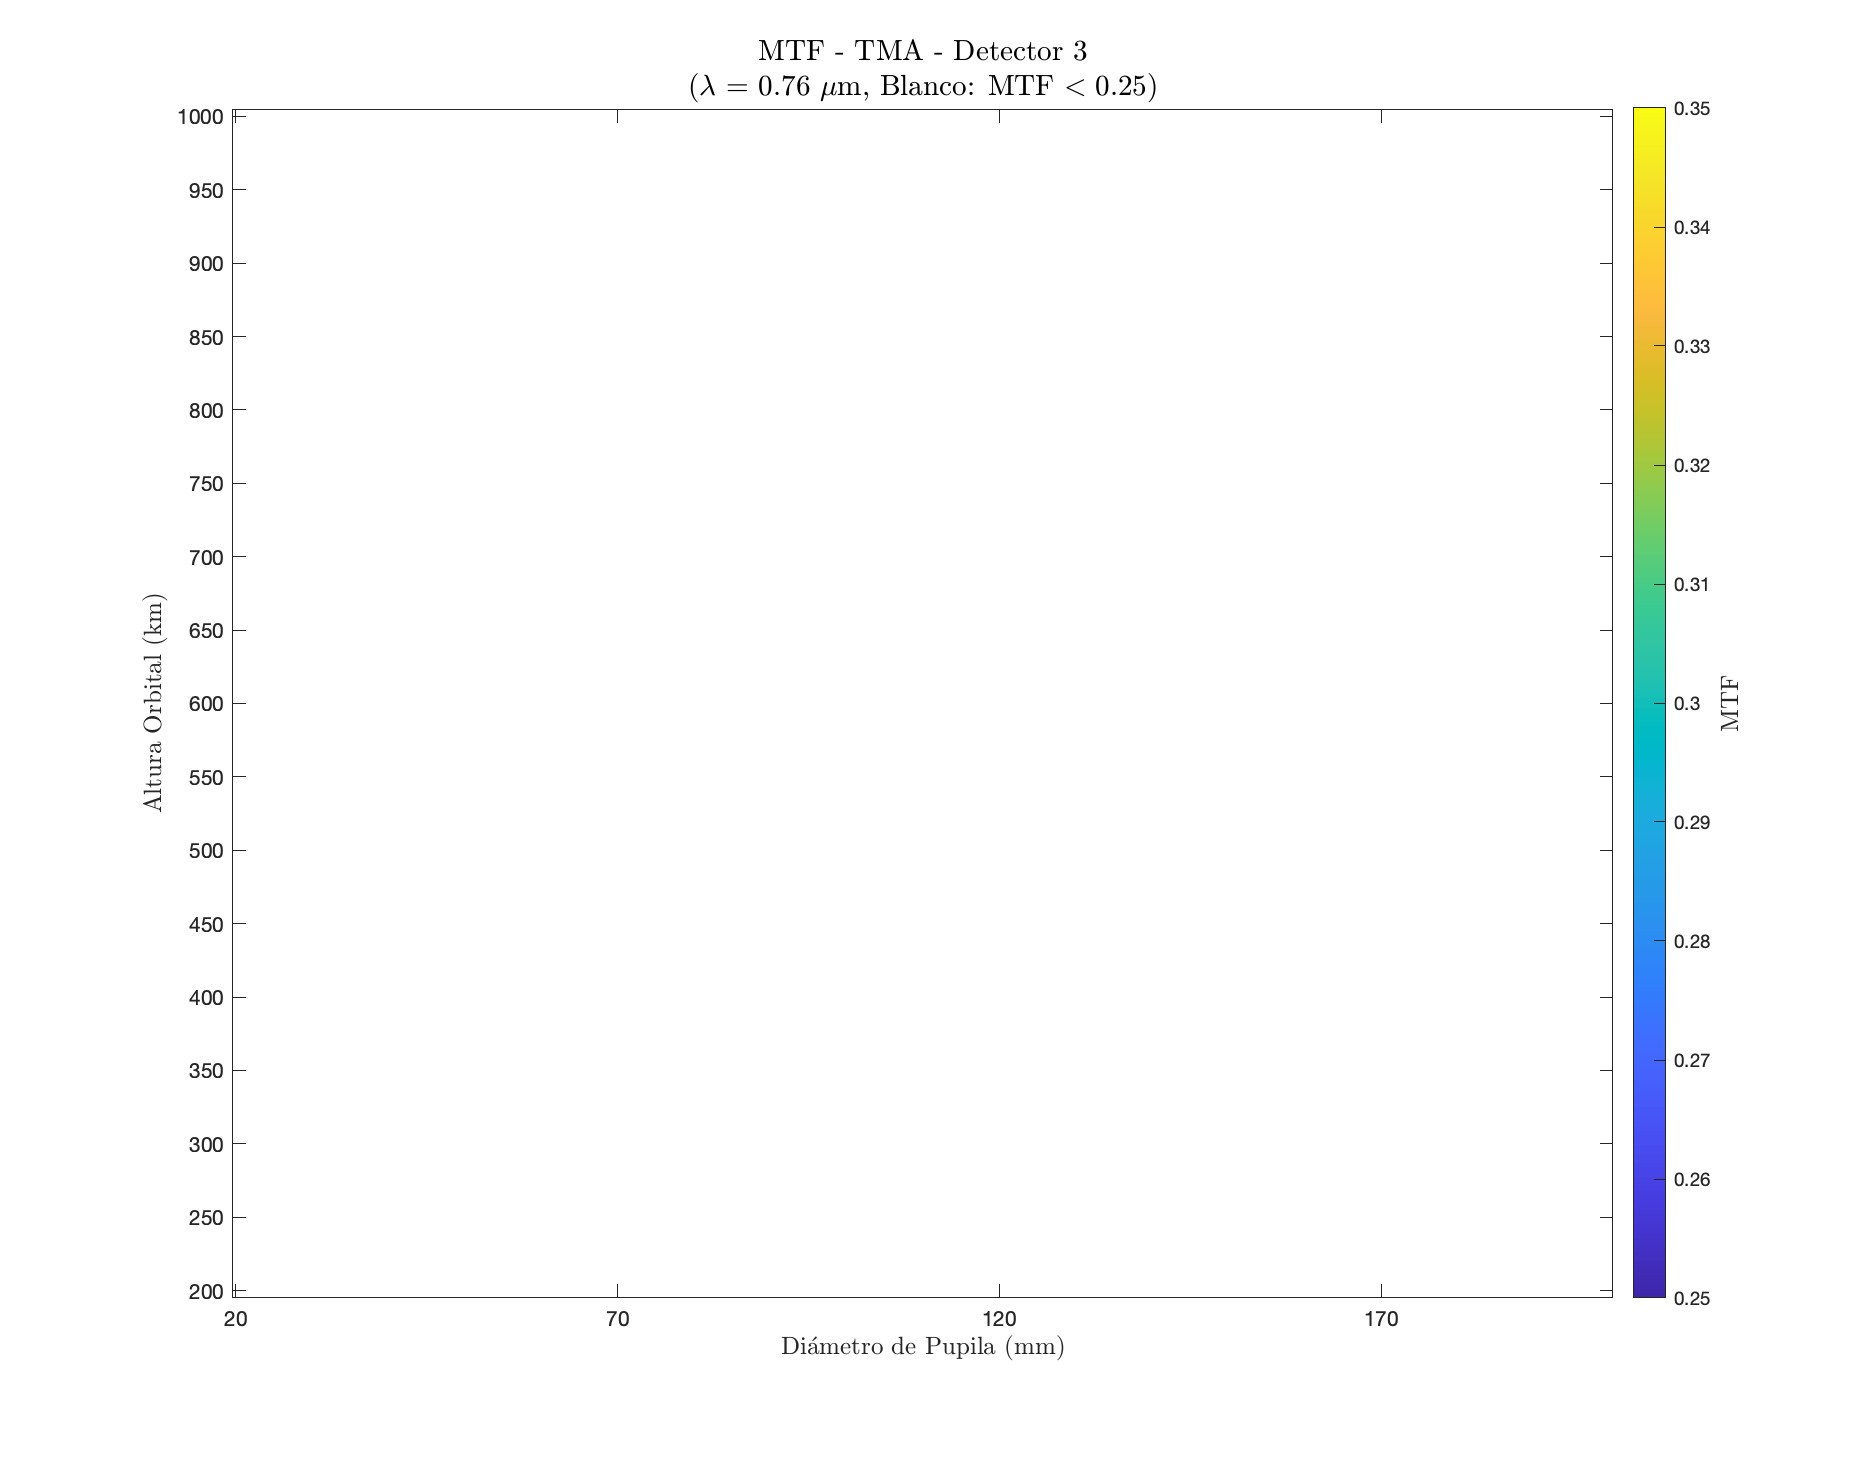
\includegraphics[width=0.48\linewidth]{4.Payload/MTF/MTF_Lambda3_Detector6_Telescopio4_heatmap.jpg} \\
\end{tabular}

\caption{Mapas de calor resultantes del calculo de MTF: Banda 0,76 \textmu m; Detector 3}
\end{figure}
\end{landscape}





%% LAMBDA 1 %%
%========================================================================================
%% DETECTOR 1
\begin{landscape}
\begin{figure}[p]
\centering
\setlength{\tabcolsep}{2pt}
\renewcommand{\arraystretch}{0}
\paragraph{Banda $1,61\ \mu m$}
\begin{tabular}{cc}
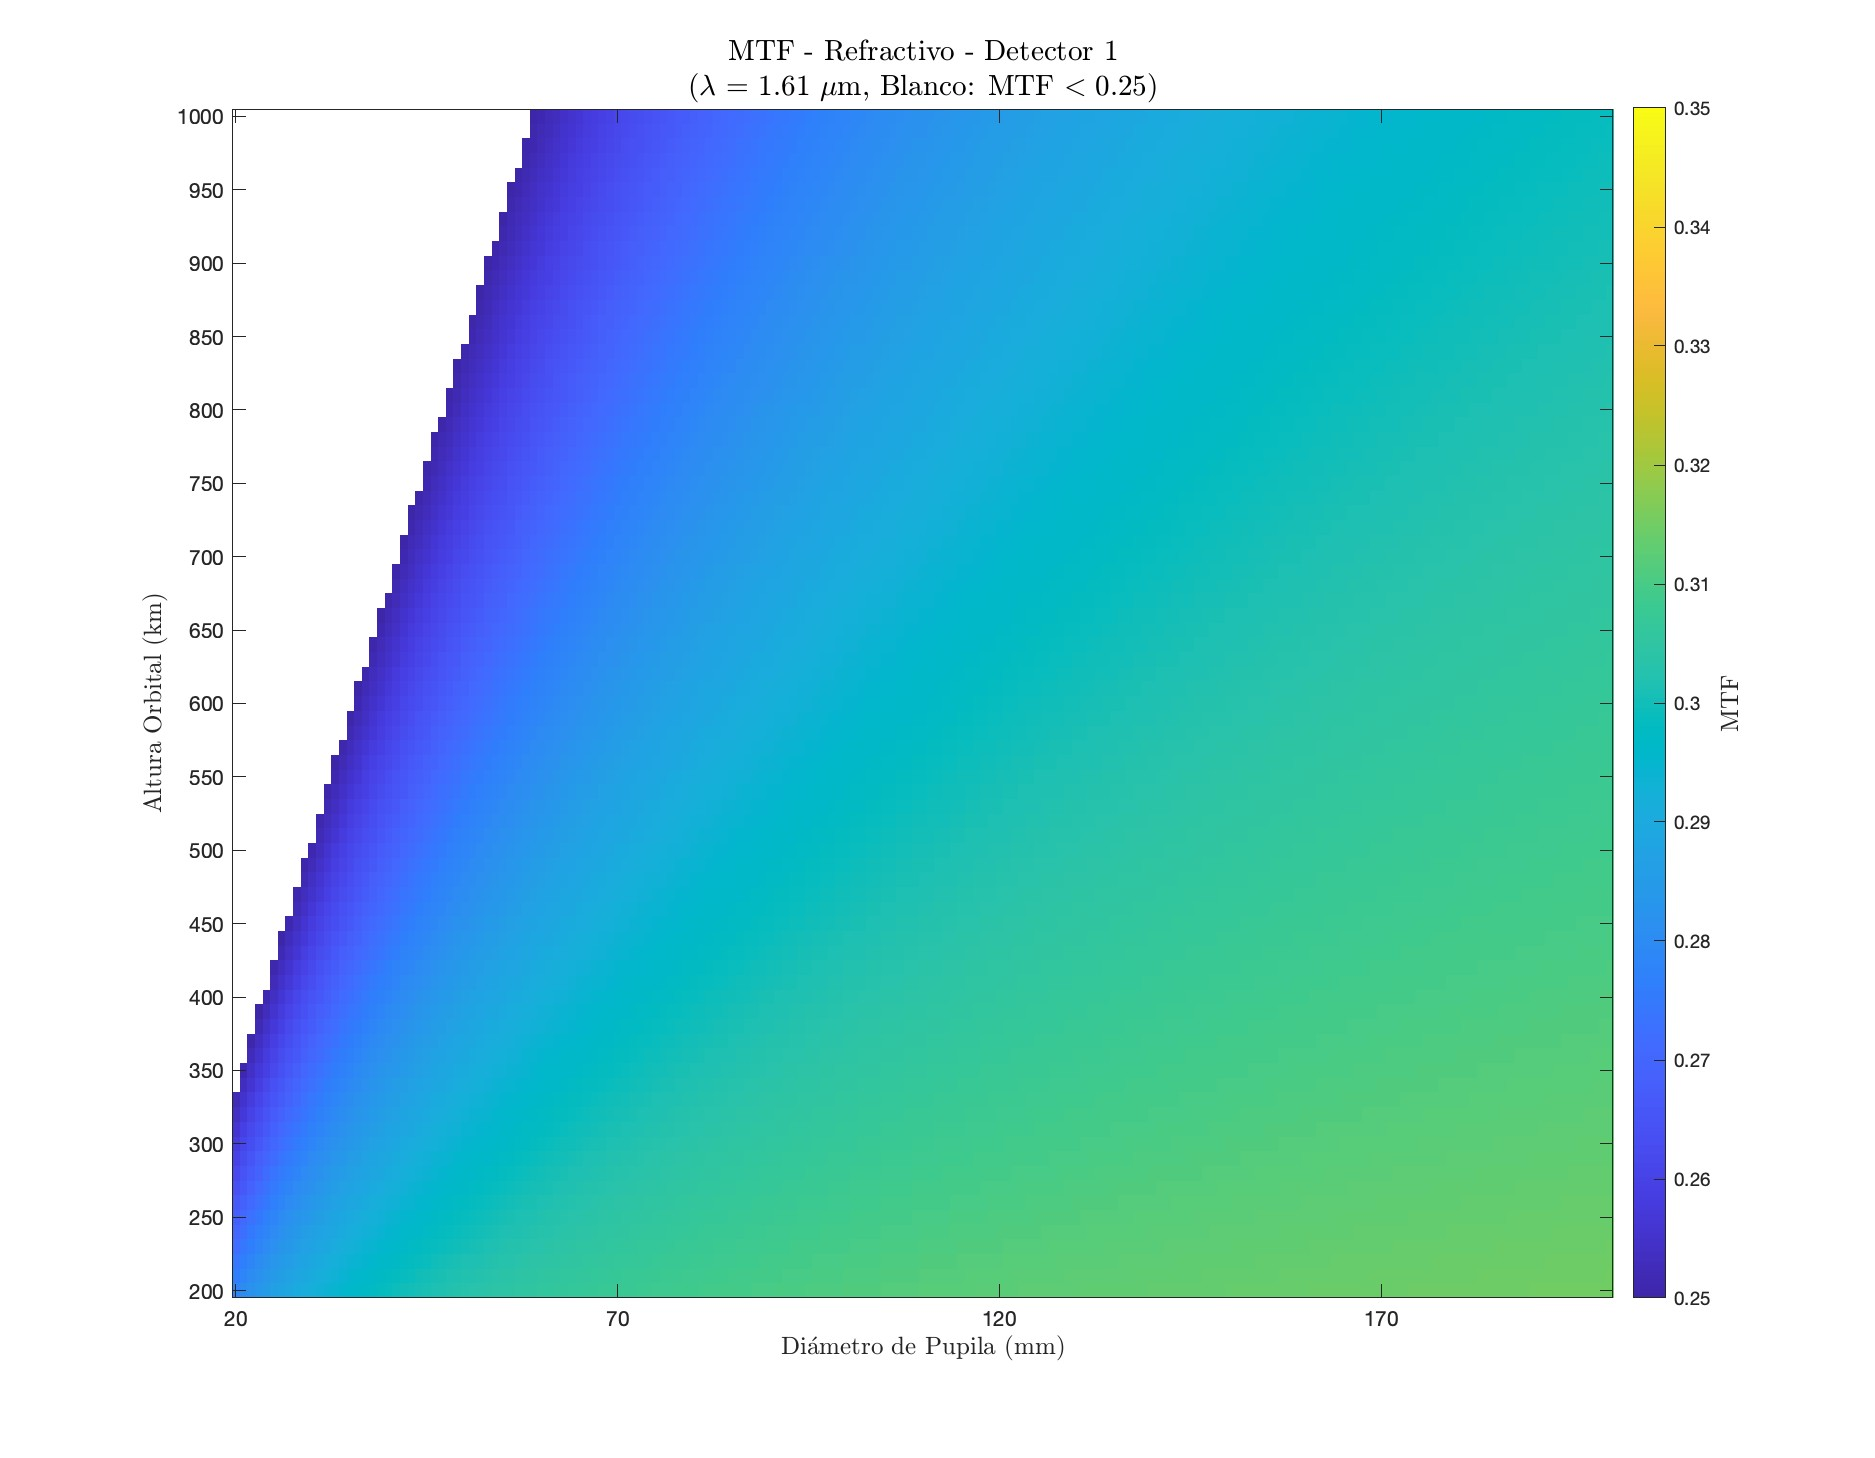
\includegraphics[width=0.48\linewidth]{4.Payload/MTF/MTF_Lambda1_Detector1_Telescopio1_heatmap.jpg} &
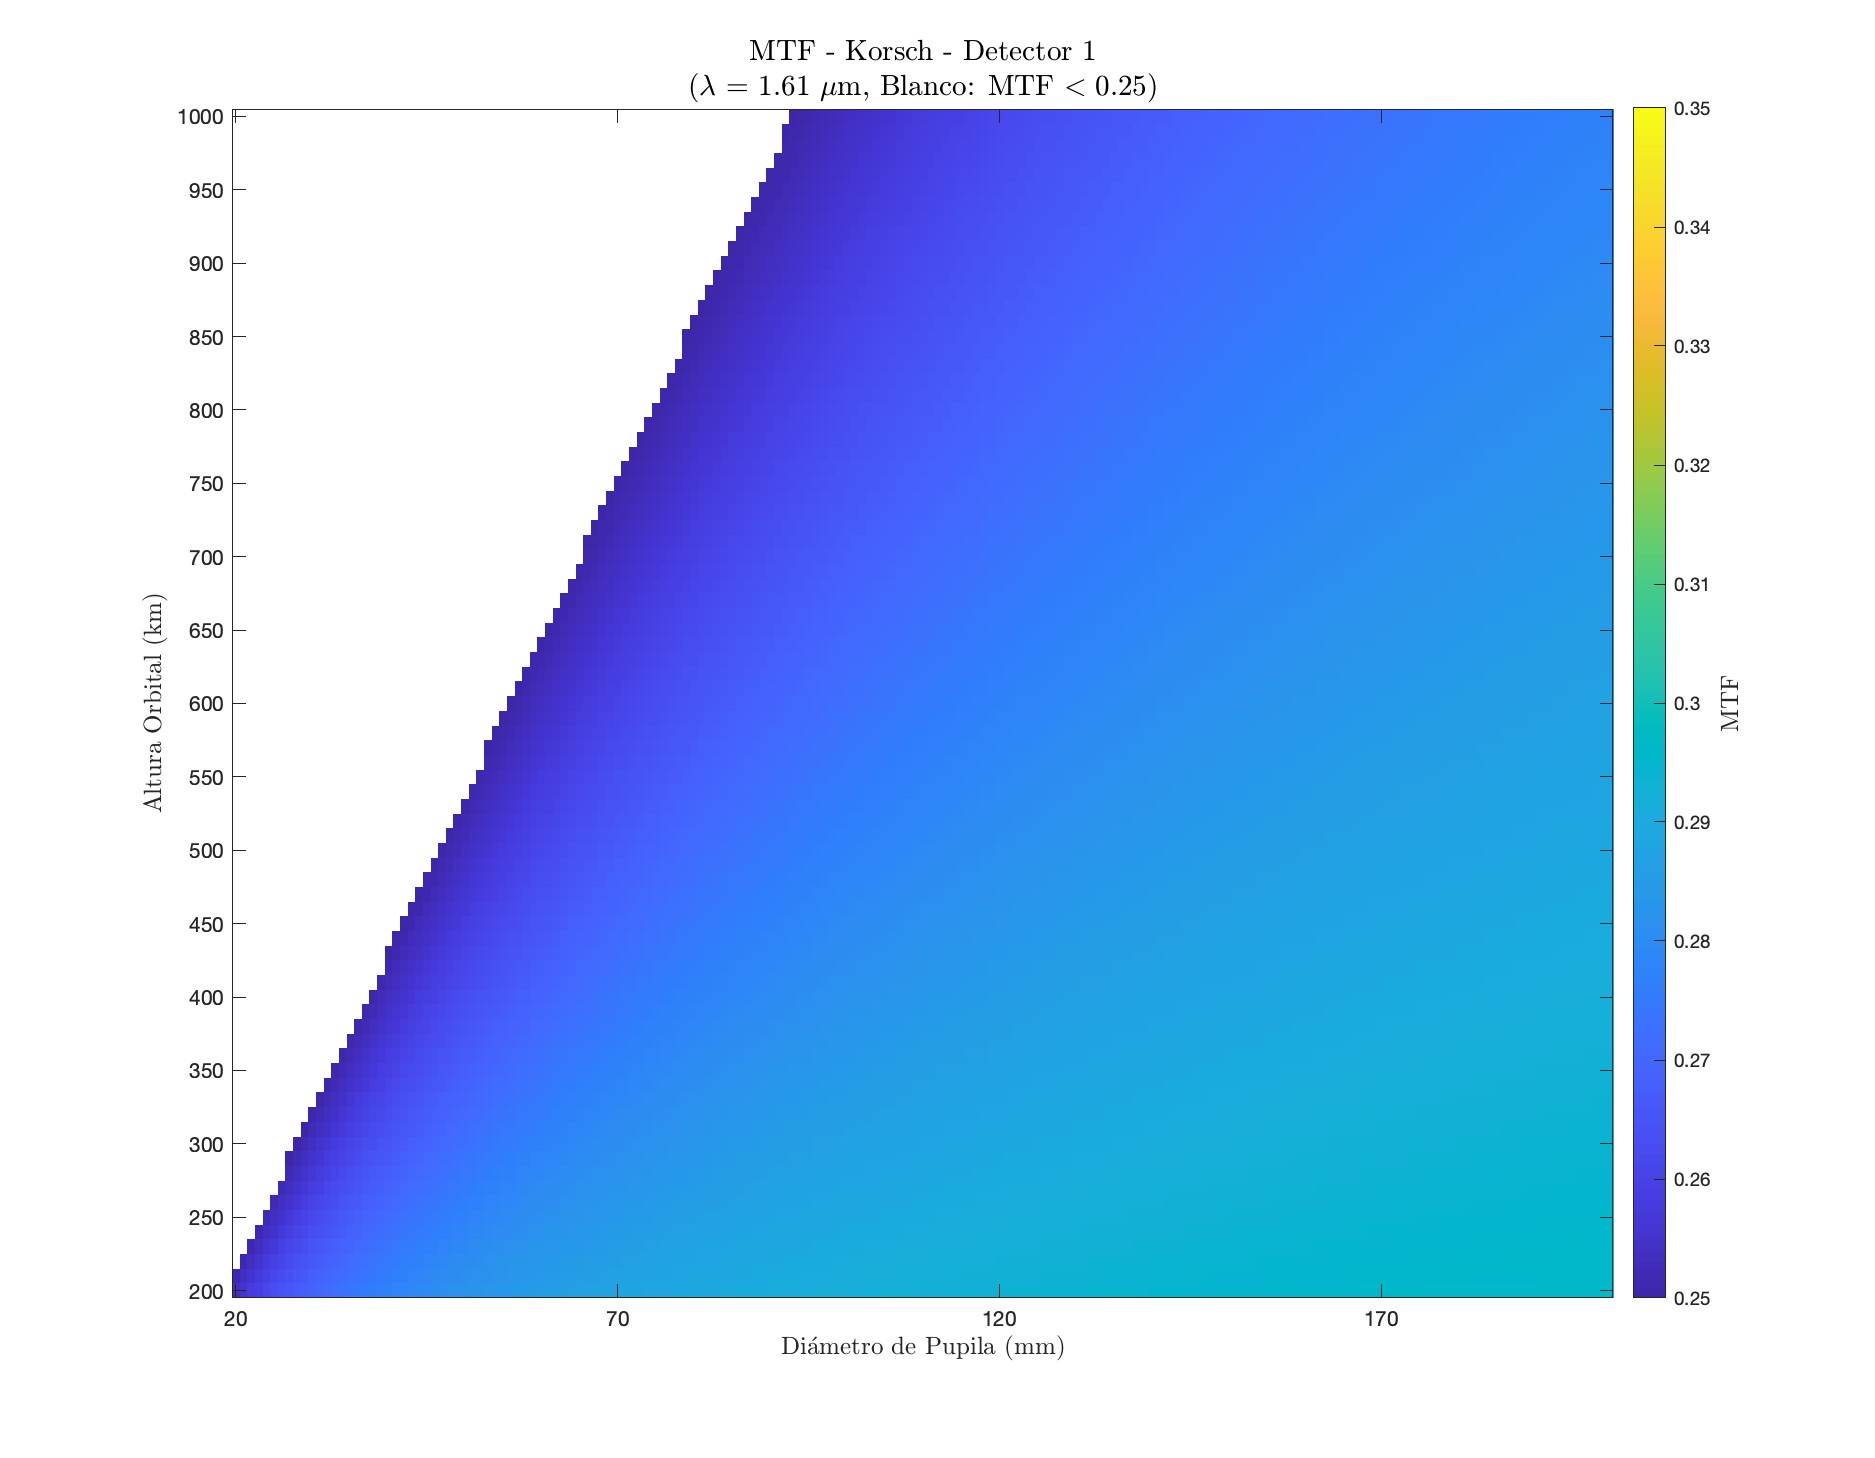
\includegraphics[width=0.48\linewidth]{4.Payload/MTF/MTF_Lambda1_Detector1_Telescopio2_heatmap.jpg} \\
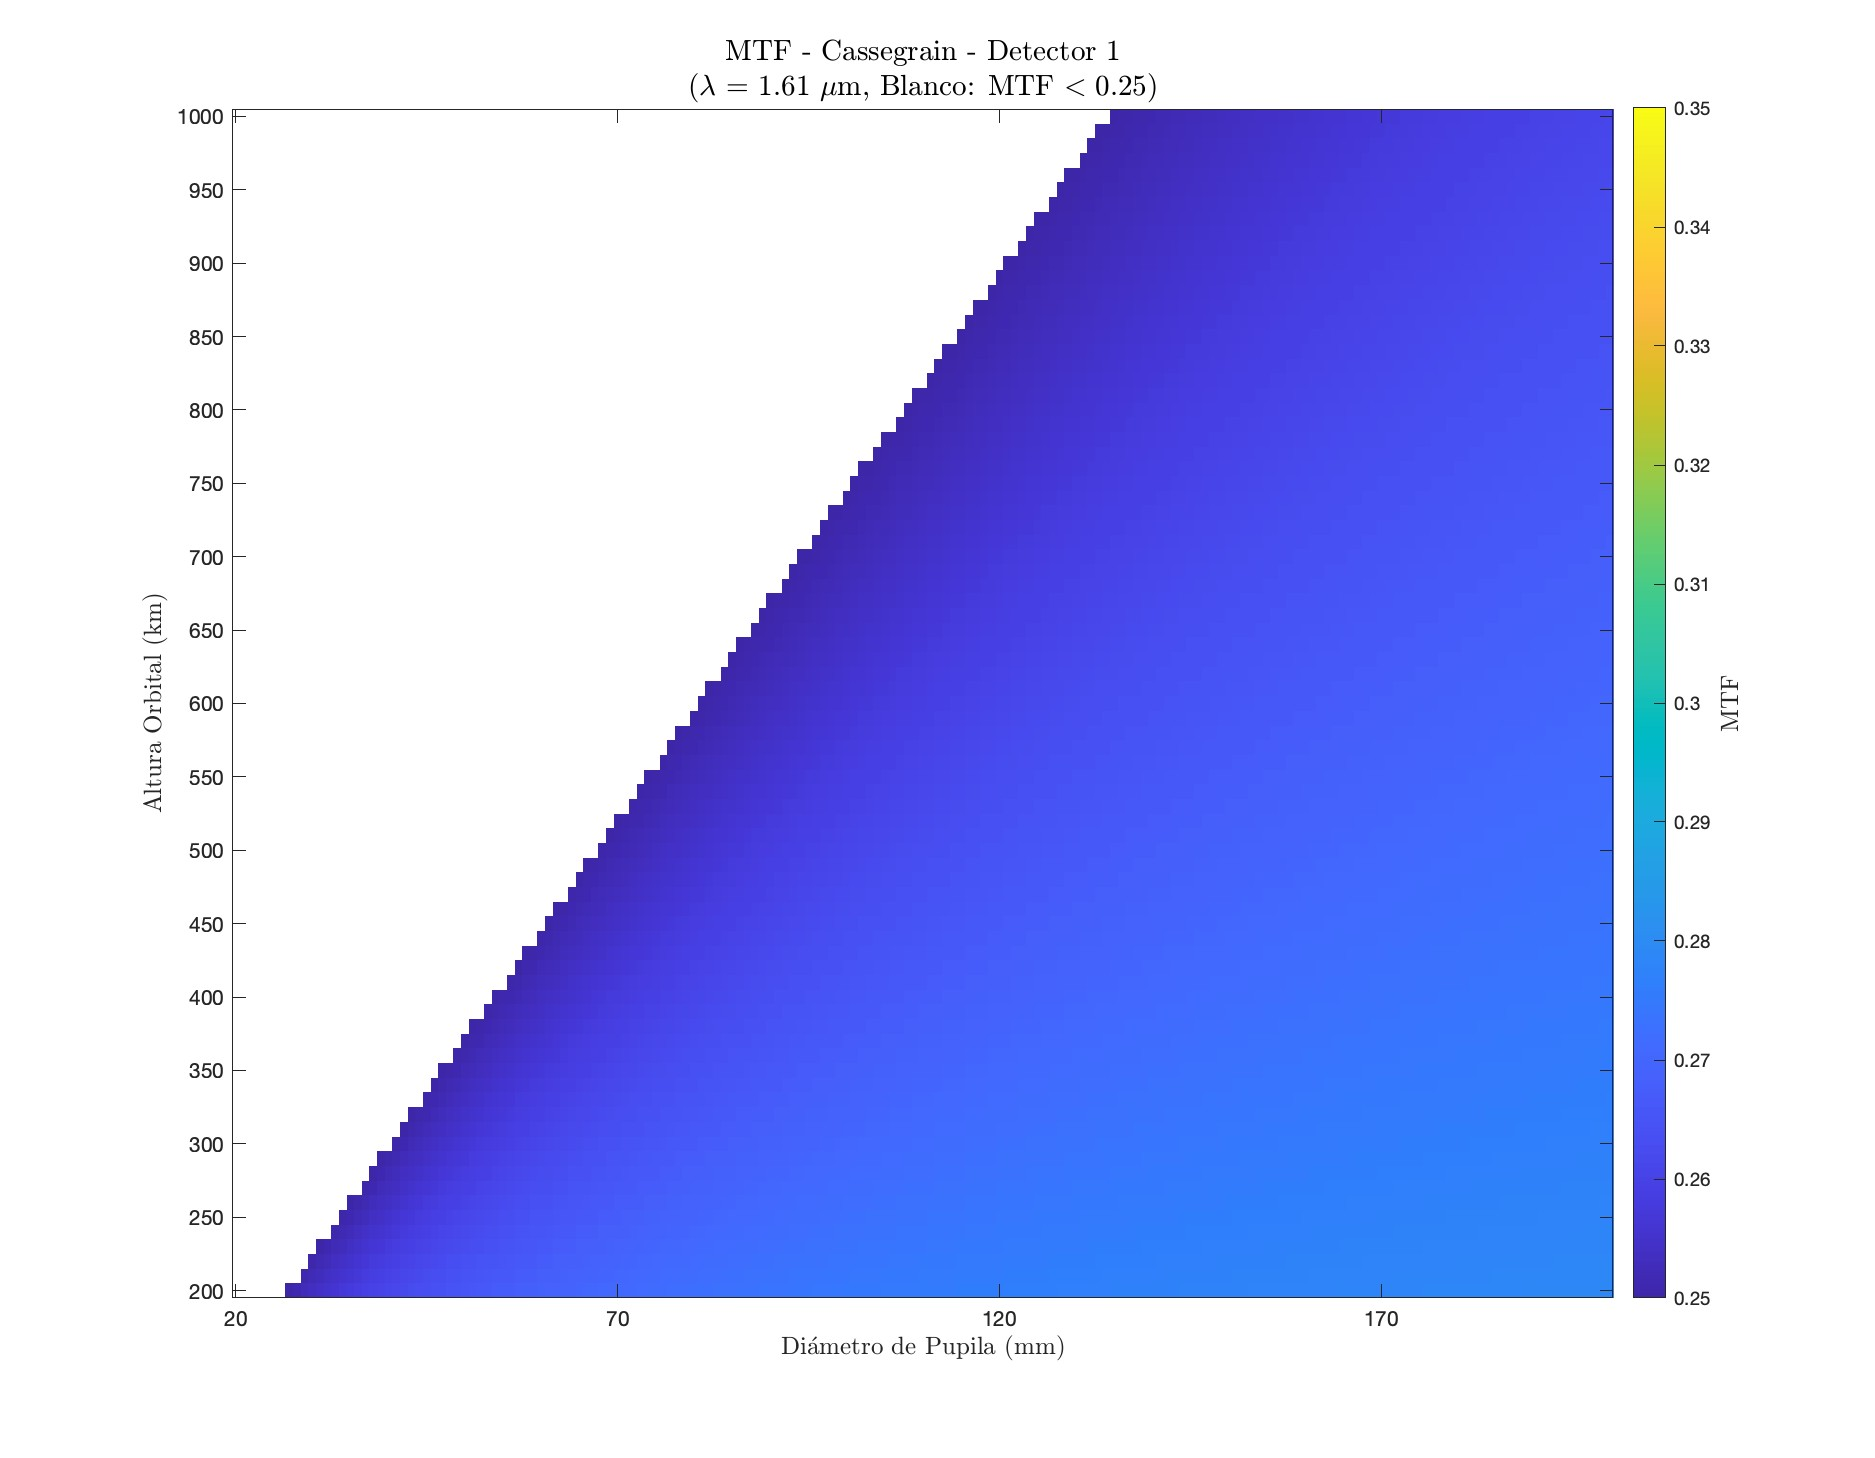
\includegraphics[width=0.48\linewidth]{4.Payload/MTF/MTF_Lambda1_Detector1_Telescopio3_heatmap.jpg} &
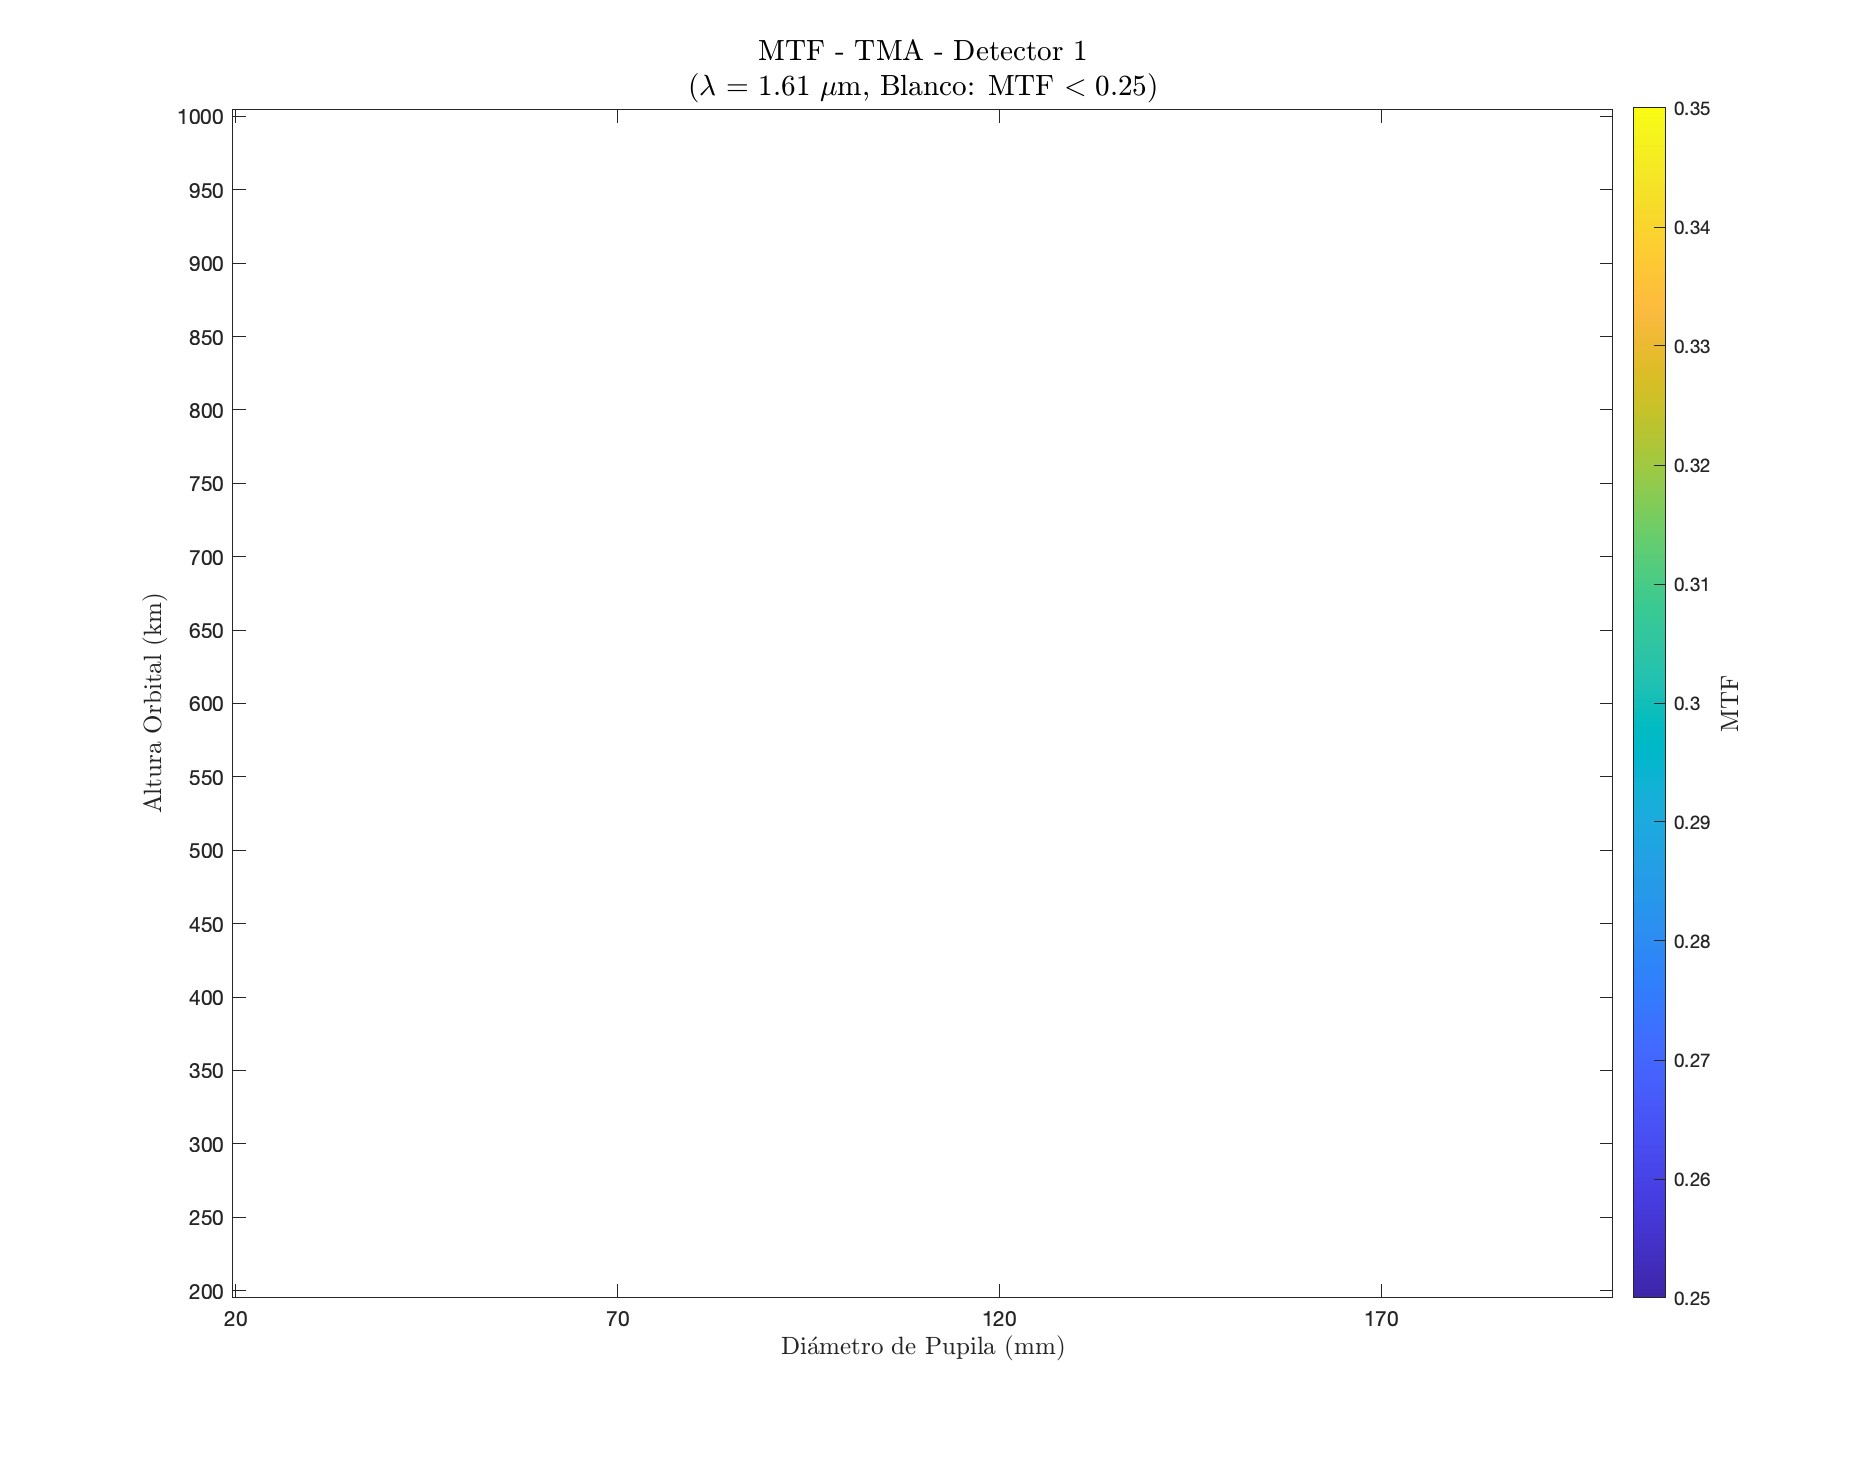
\includegraphics[width=0.48\linewidth]{4.Payload/MTF/MTF_Lambda1_Detector1_Telescopio4_heatmap.jpg} \\
\end{tabular}

\caption{Mapas de calor resultantes del calculo de MTF: Banda 1,61 \textmu m; Detector 1}
\end{figure}
\end{landscape}


%% DETECTOR 2
\begin{landscape}
\begin{figure}[p]
\centering
\setlength{\tabcolsep}{2pt}
\renewcommand{\arraystretch}{0}

\begin{tabular}{cc}
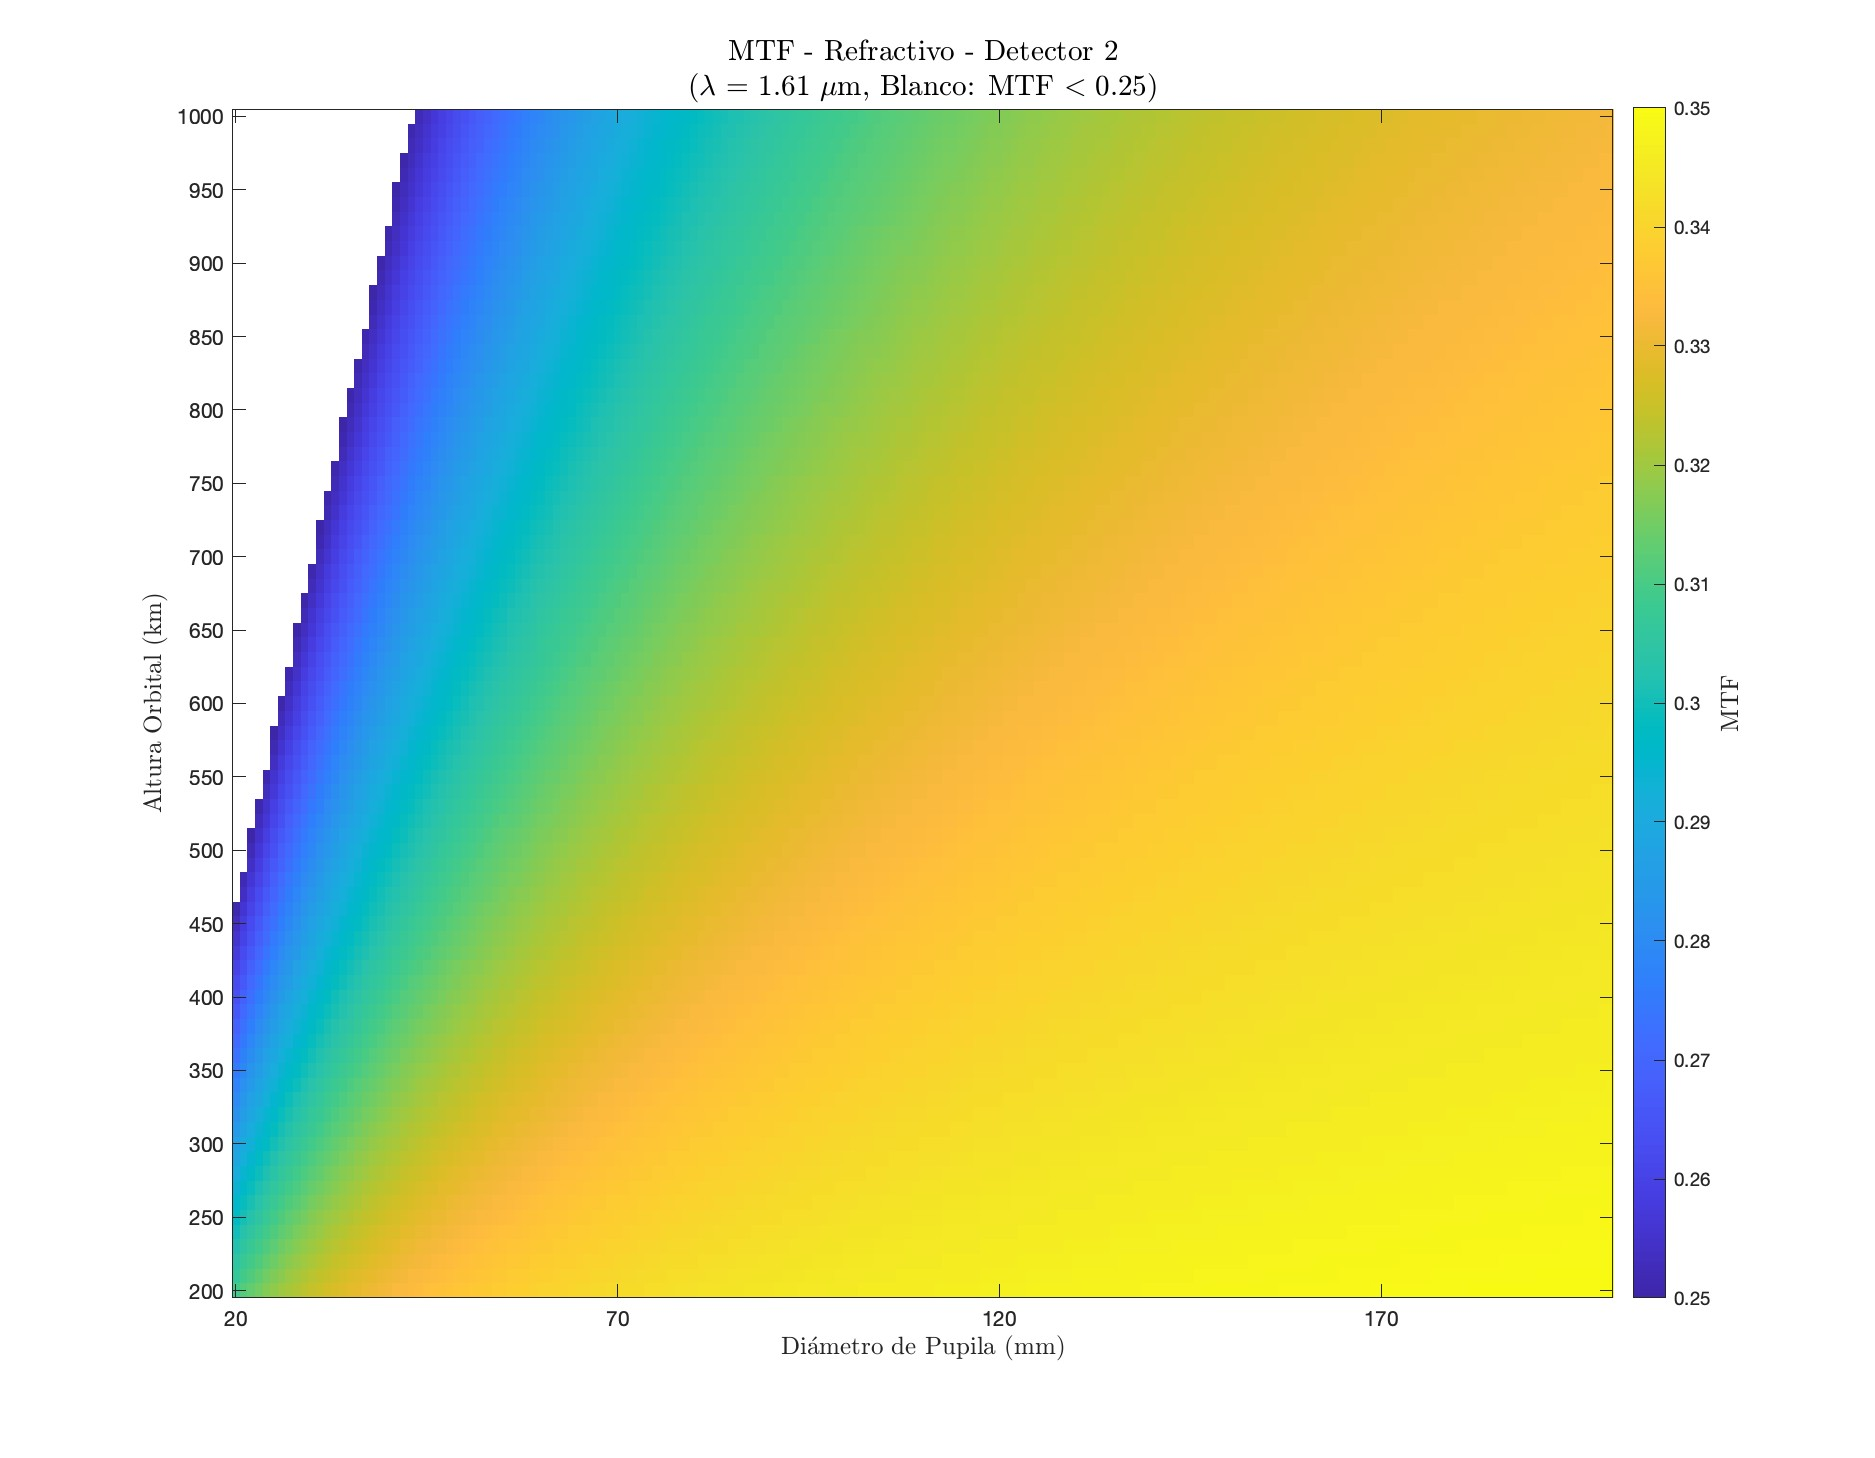
\includegraphics[width=0.48\linewidth]{4.Payload/MTF/MTF_Lambda1_Detector2_Telescopio1_heatmap.jpg} &
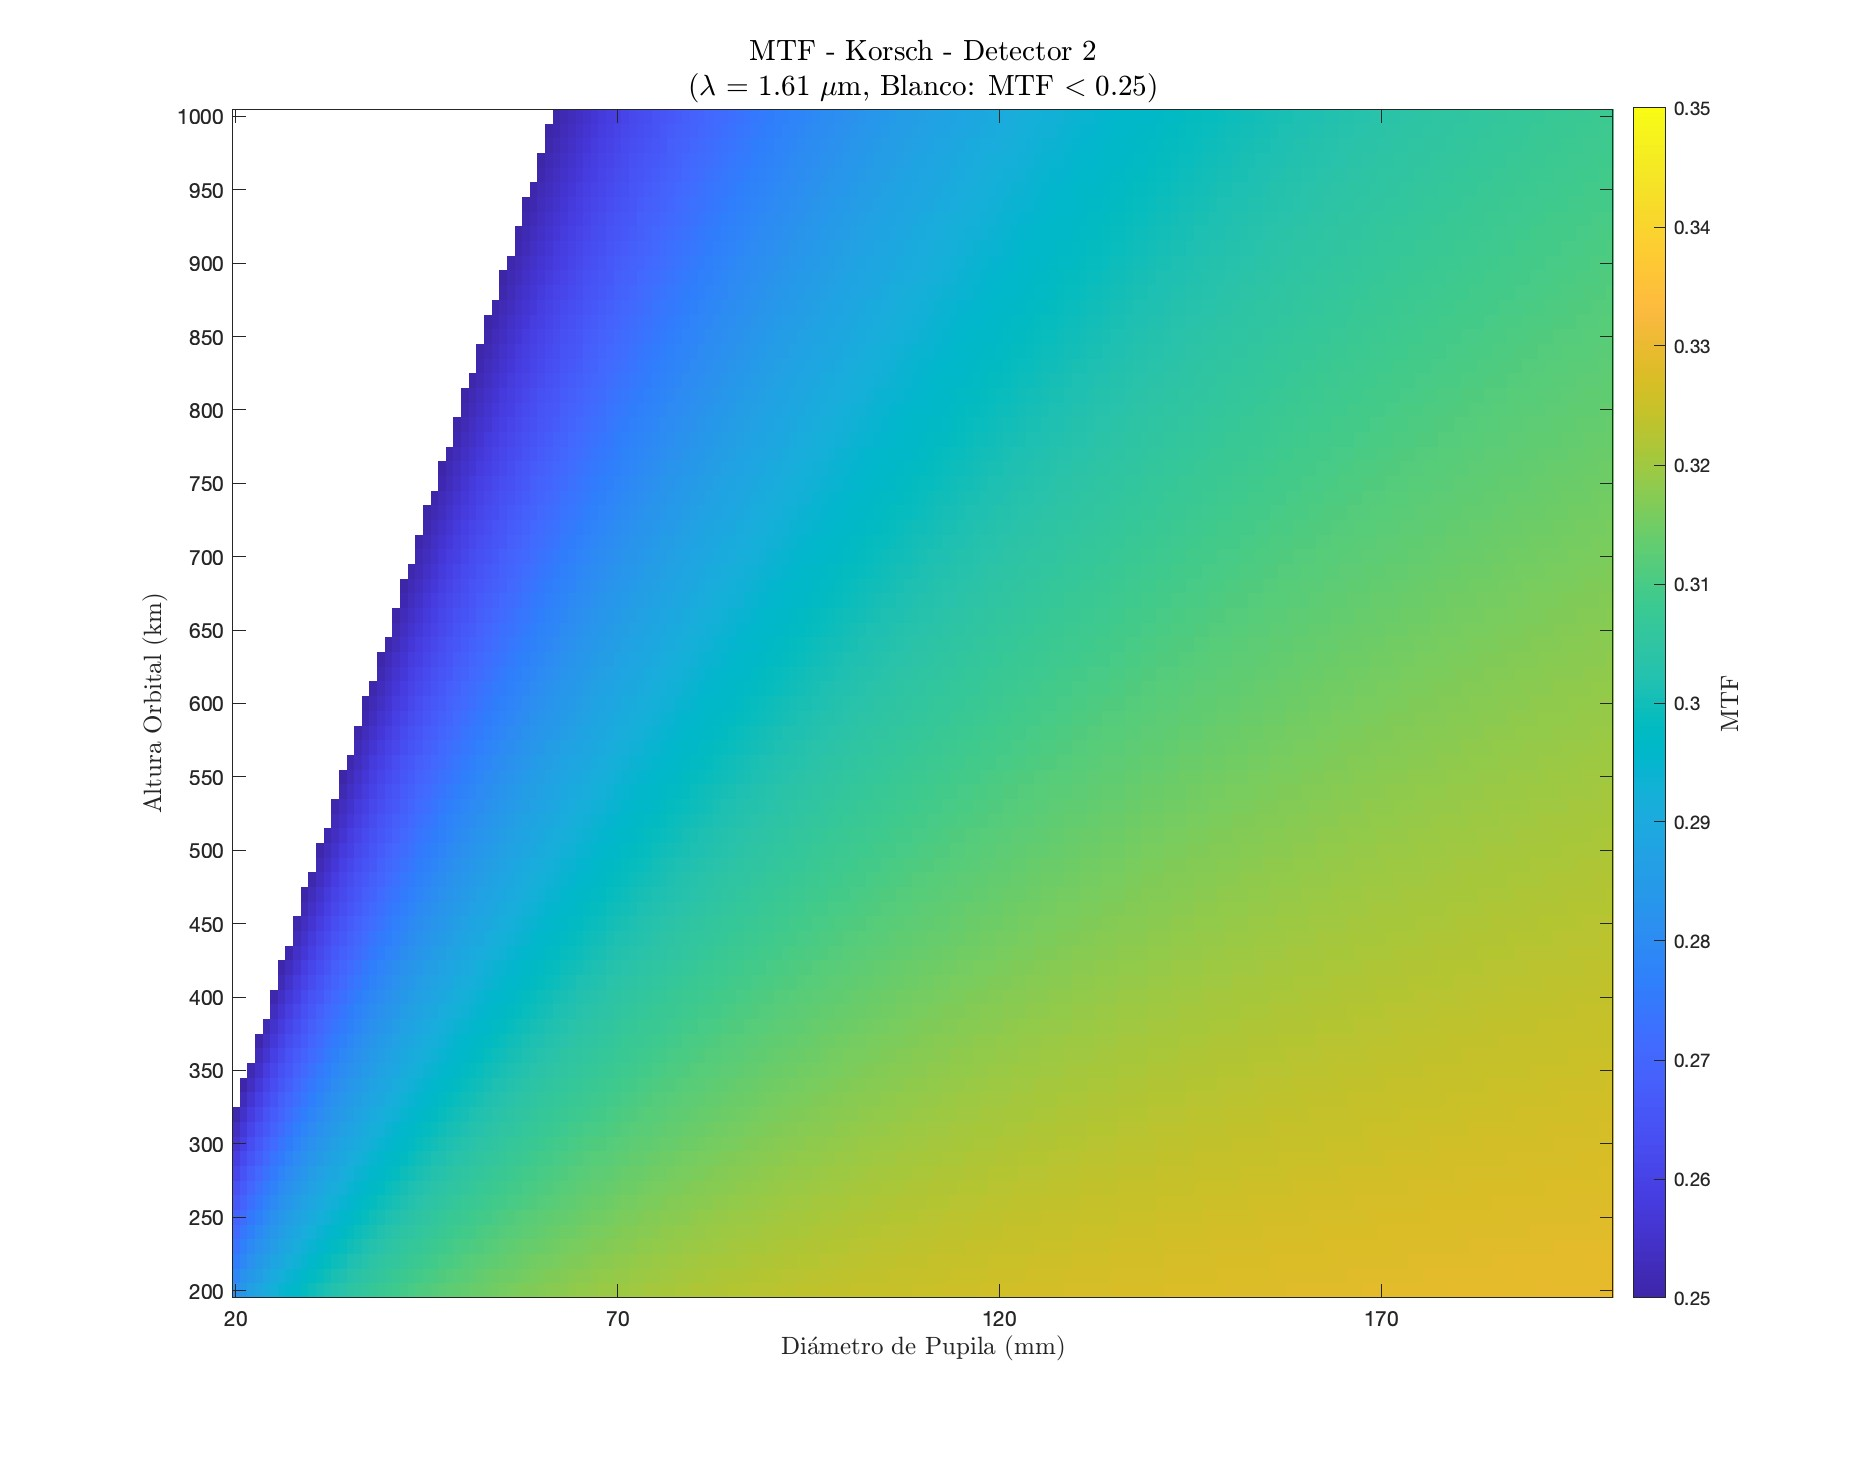
\includegraphics[width=0.48\linewidth]{4.Payload/MTF/MTF_Lambda1_Detector2_Telescopio2_heatmap.jpg} \\
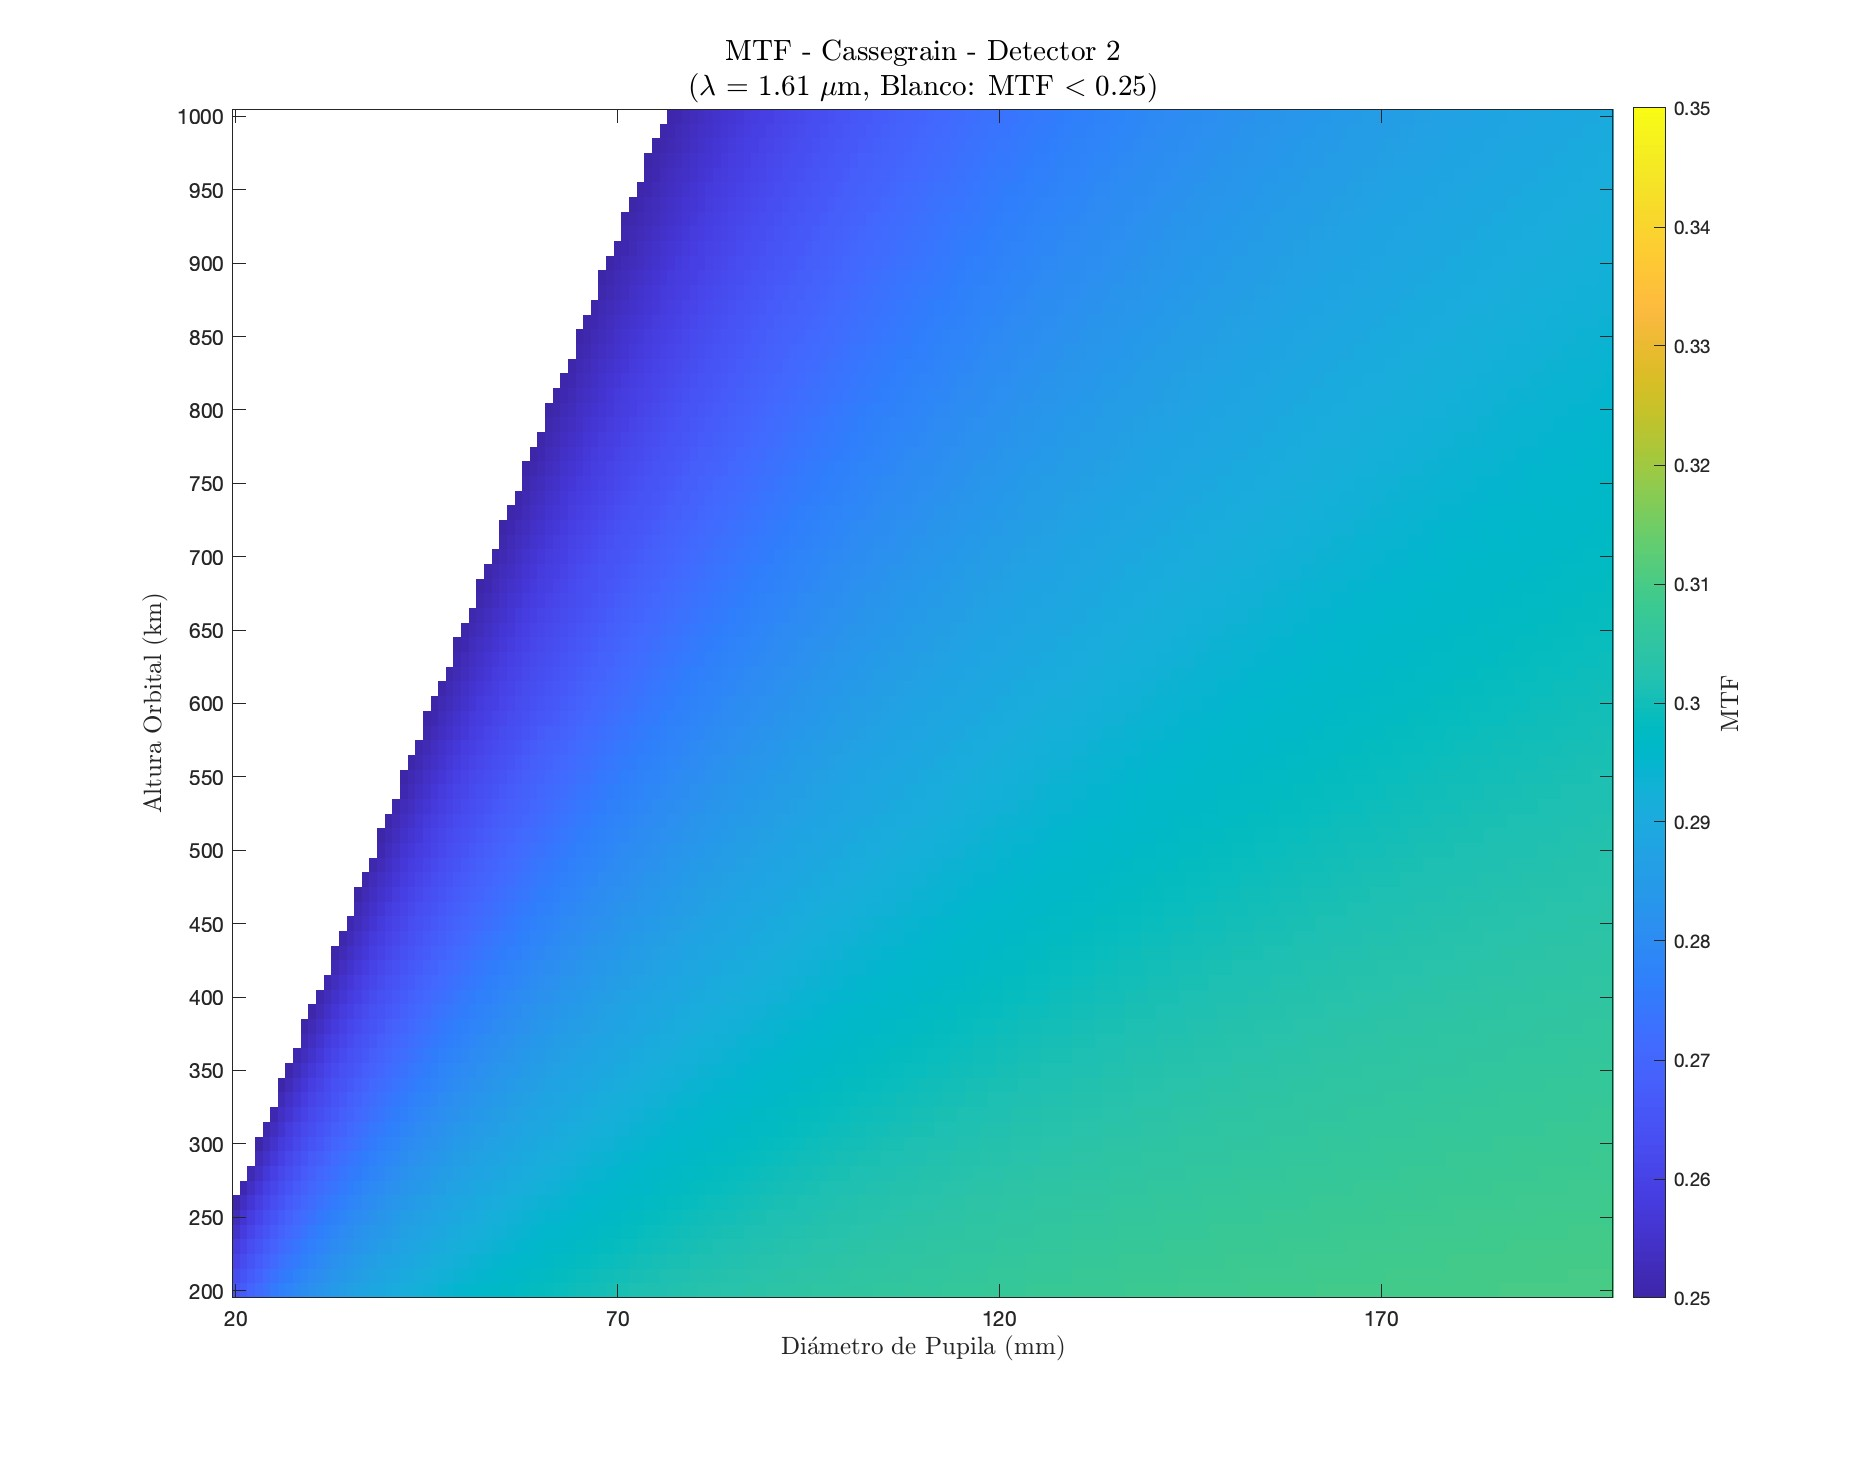
\includegraphics[width=0.48\linewidth]{4.Payload/MTF/MTF_Lambda1_Detector2_Telescopio3_heatmap.jpg} &
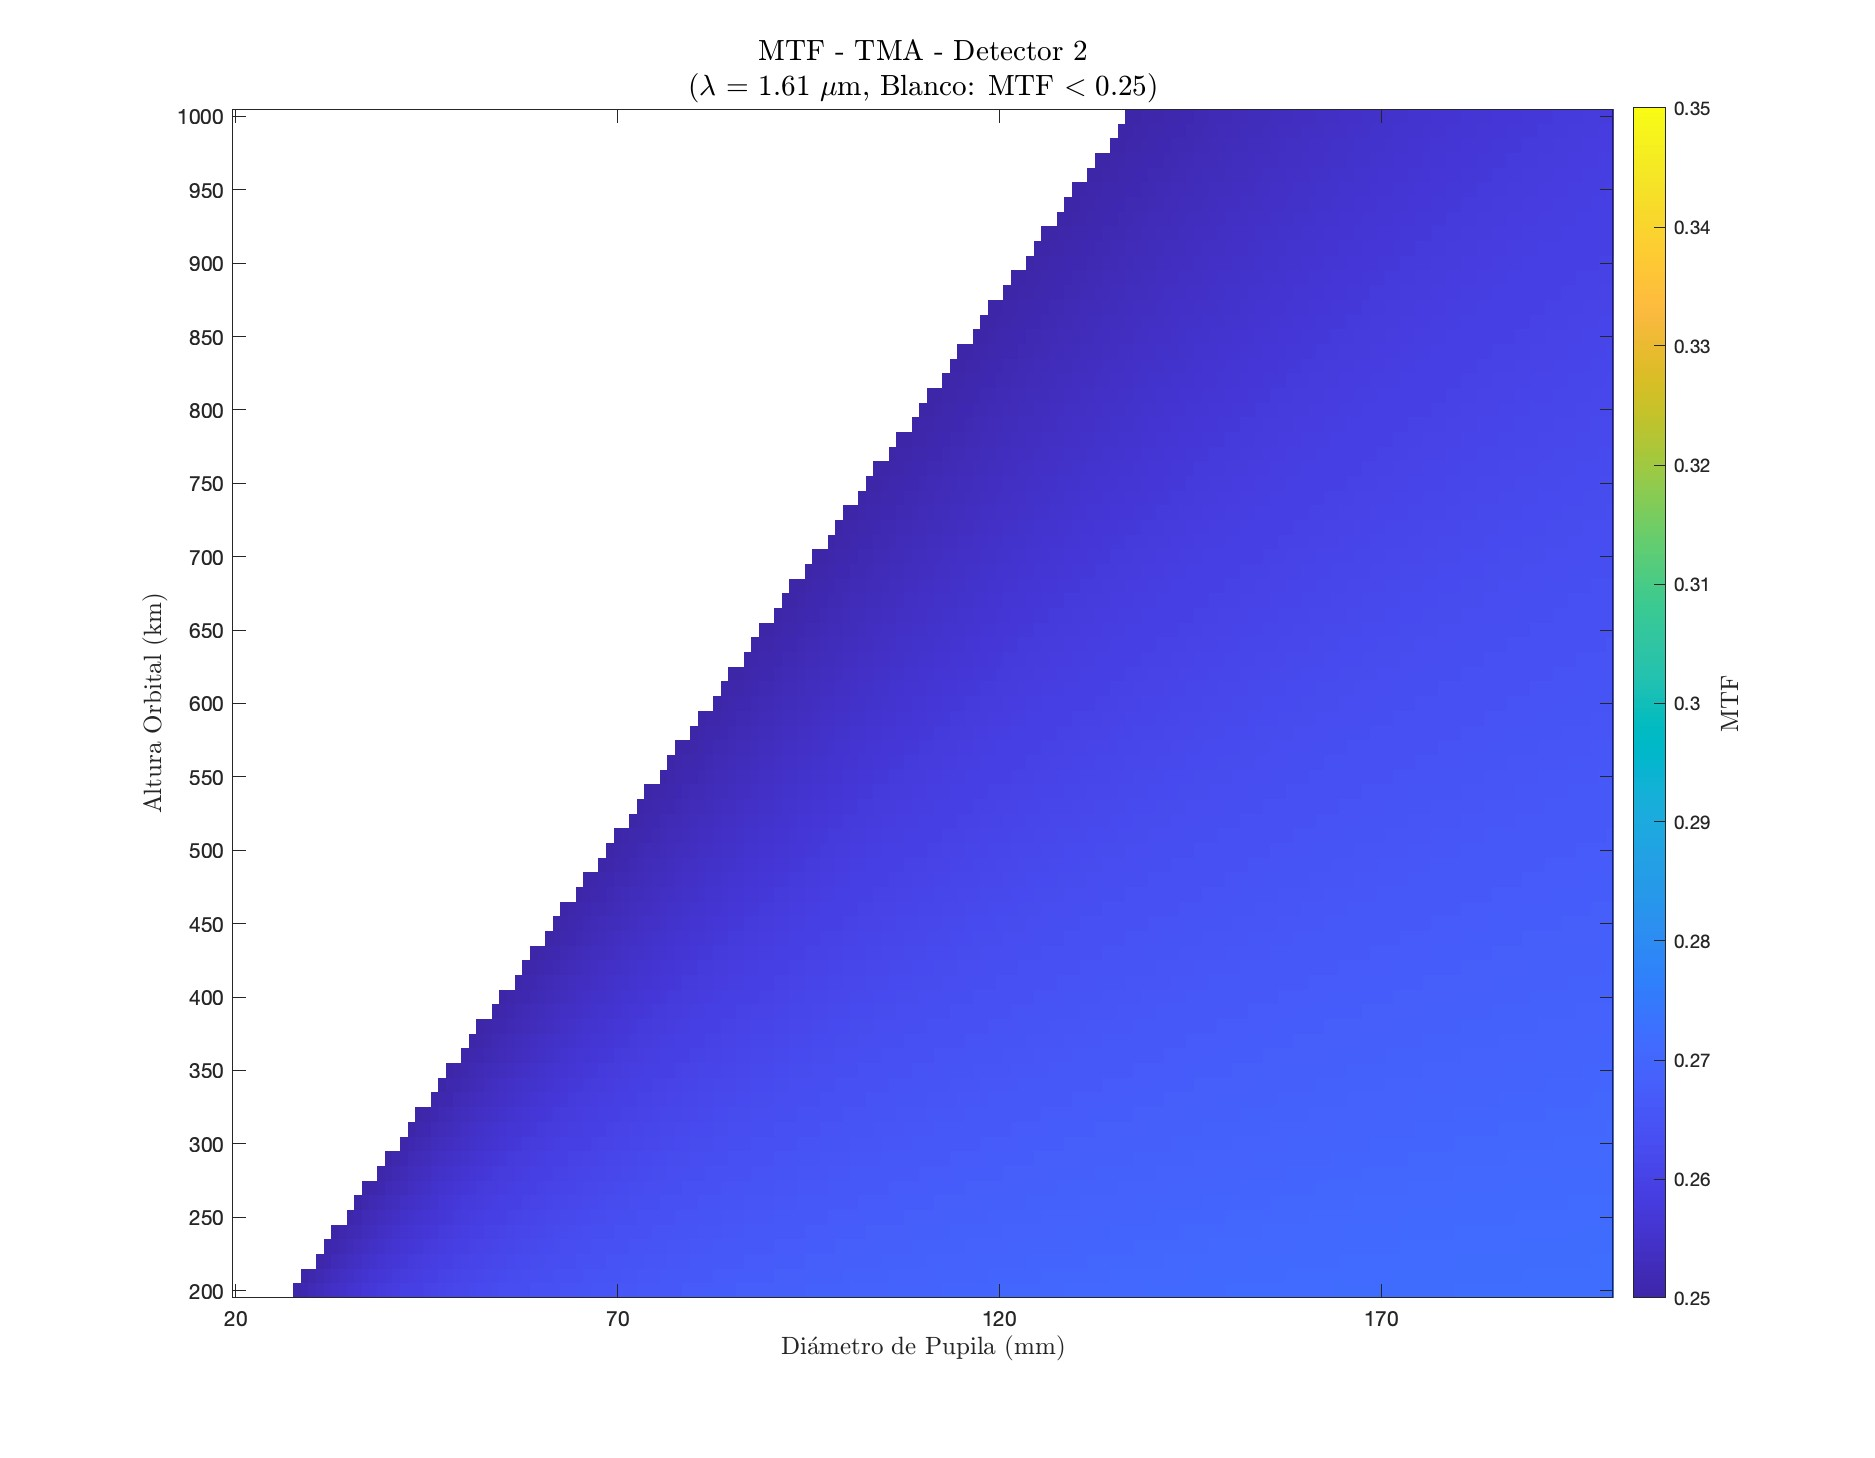
\includegraphics[width=0.48\linewidth]{4.Payload/MTF/MTF_Lambda1_Detector2_Telescopio4_heatmap.jpg} \\
\end{tabular}

\caption{Mapas de calor resultantes del calculo de MTF: Banda 1,61 \textmu m; Detector 2}
\end{figure}
\end{landscape}


%% DETECTOR 3
\begin{landscape}
\begin{figure}[p]
\centering
\setlength{\tabcolsep}{2pt}
\renewcommand{\arraystretch}{0}

\begin{tabular}{cc}
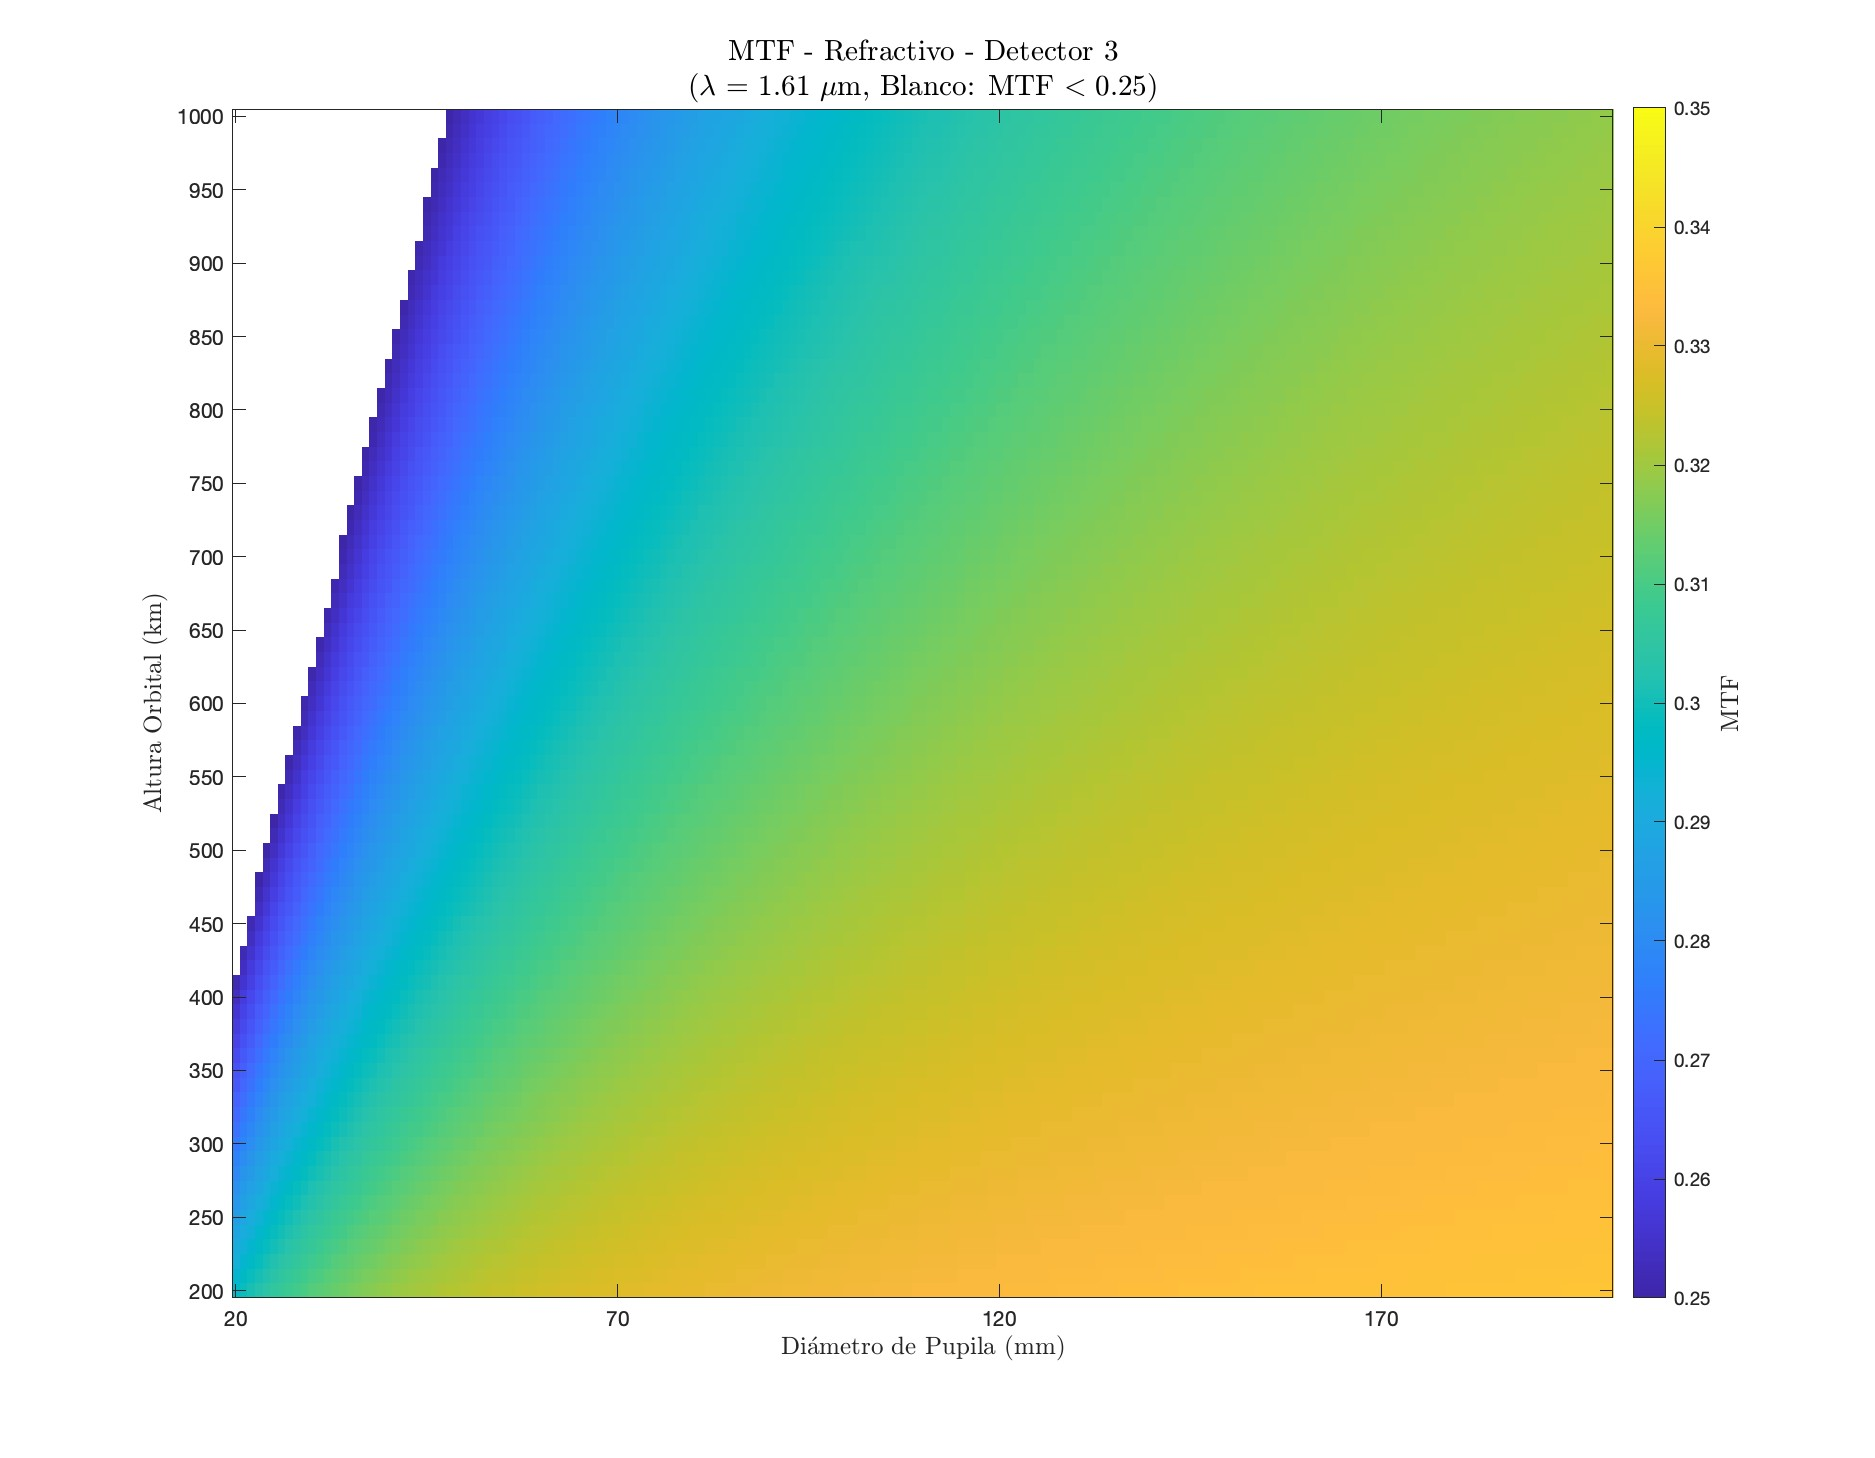
\includegraphics[width=0.48\linewidth]{4.Payload/MTF/MTF_Lambda1_Detector3_Telescopio1_heatmap.jpg} &
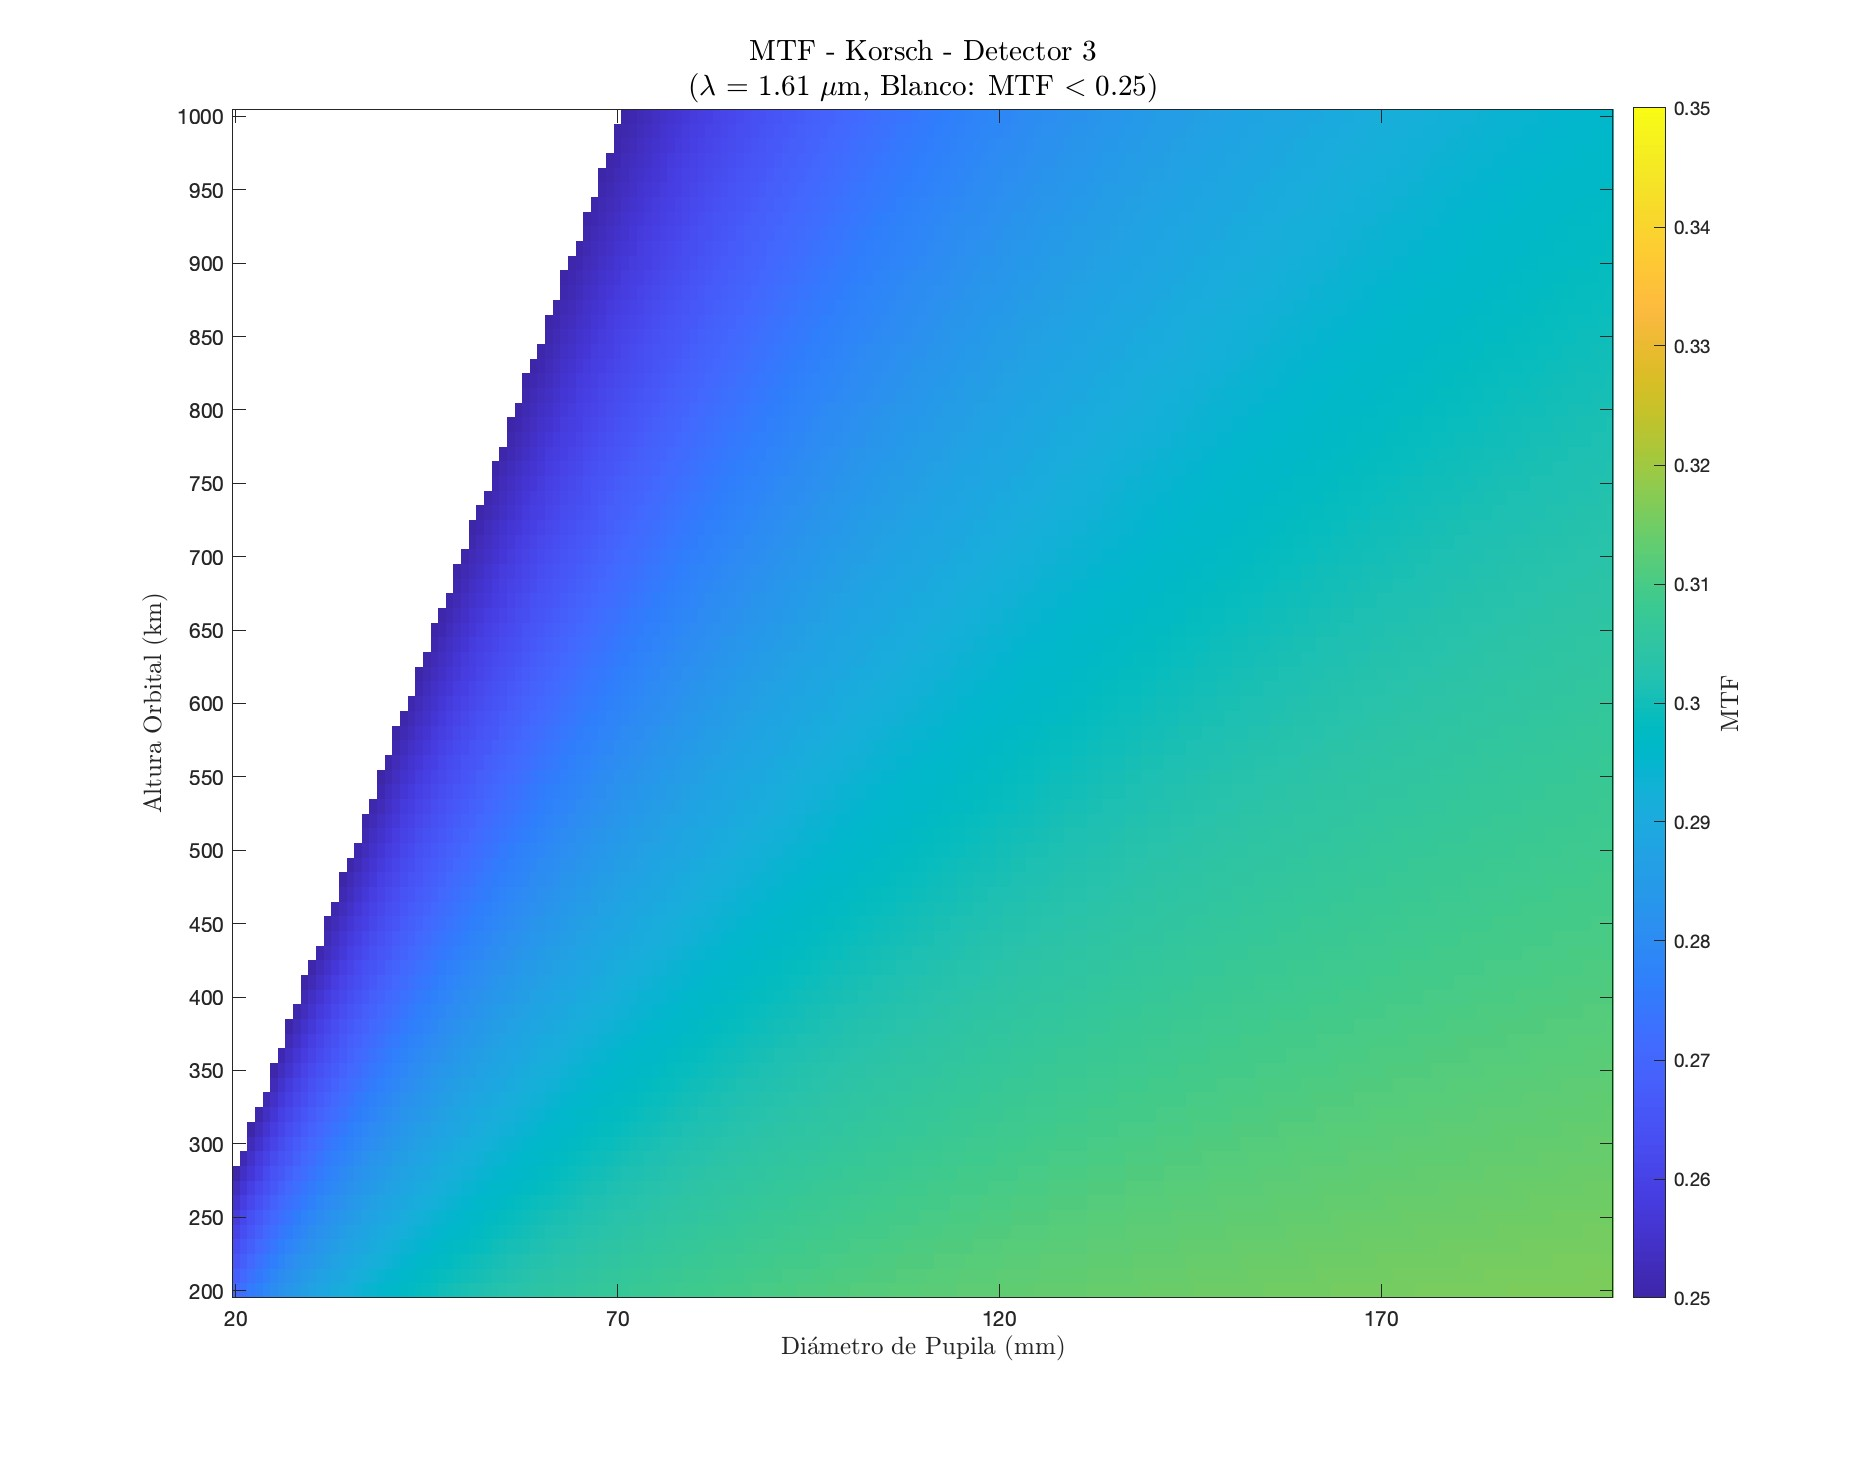
\includegraphics[width=0.48\linewidth]{4.Payload/MTF/MTF_Lambda1_Detector3_Telescopio2_heatmap.jpg} \\
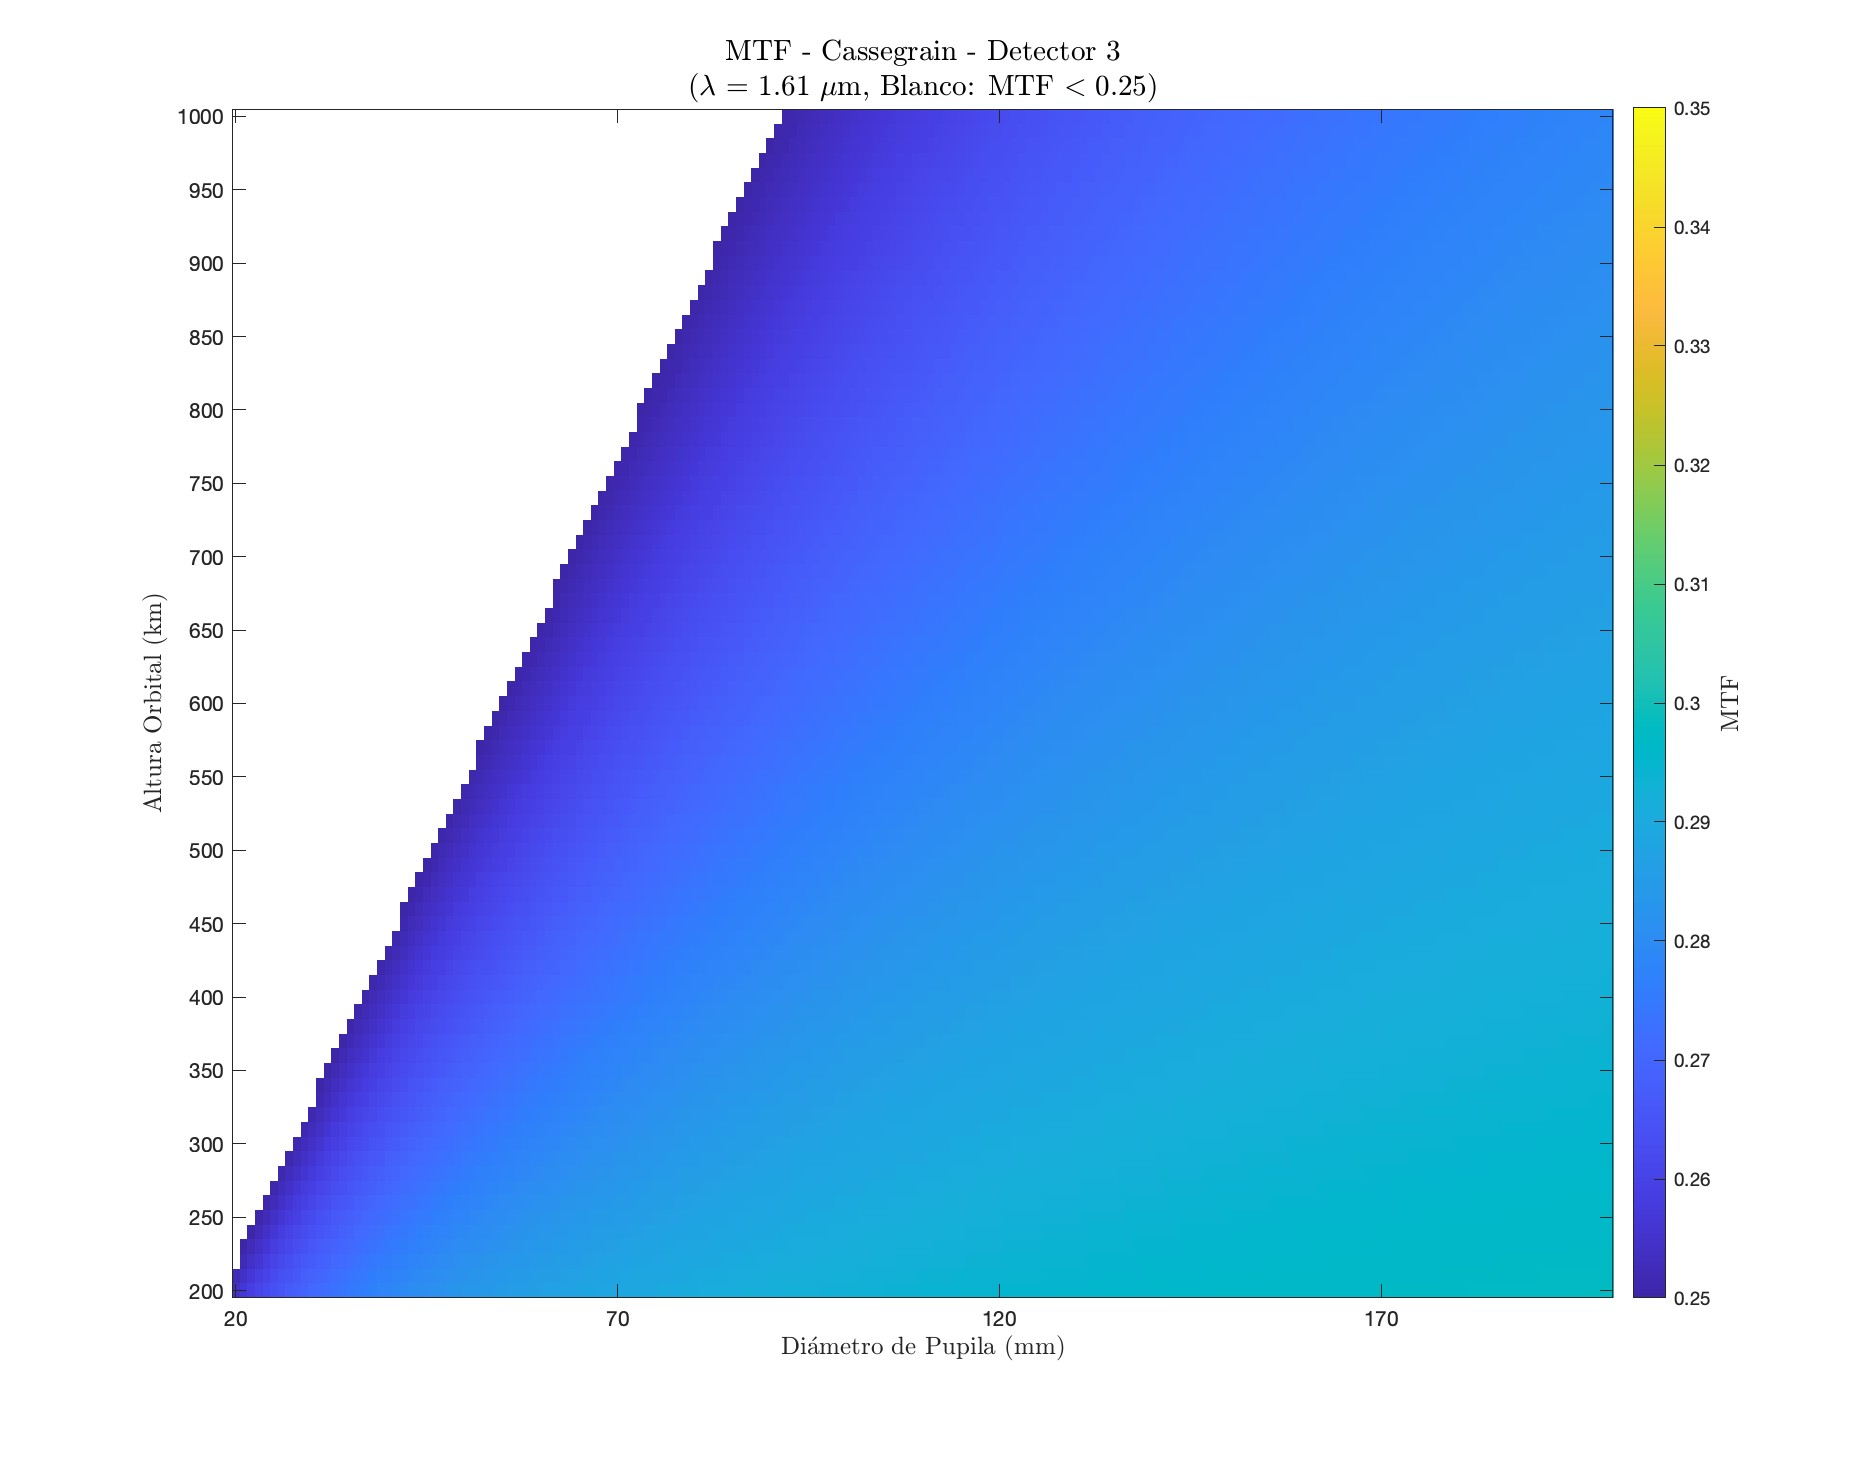
\includegraphics[width=0.48\linewidth]{4.Payload/MTF/MTF_Lambda1_Detector3_Telescopio3_heatmap.jpg} &
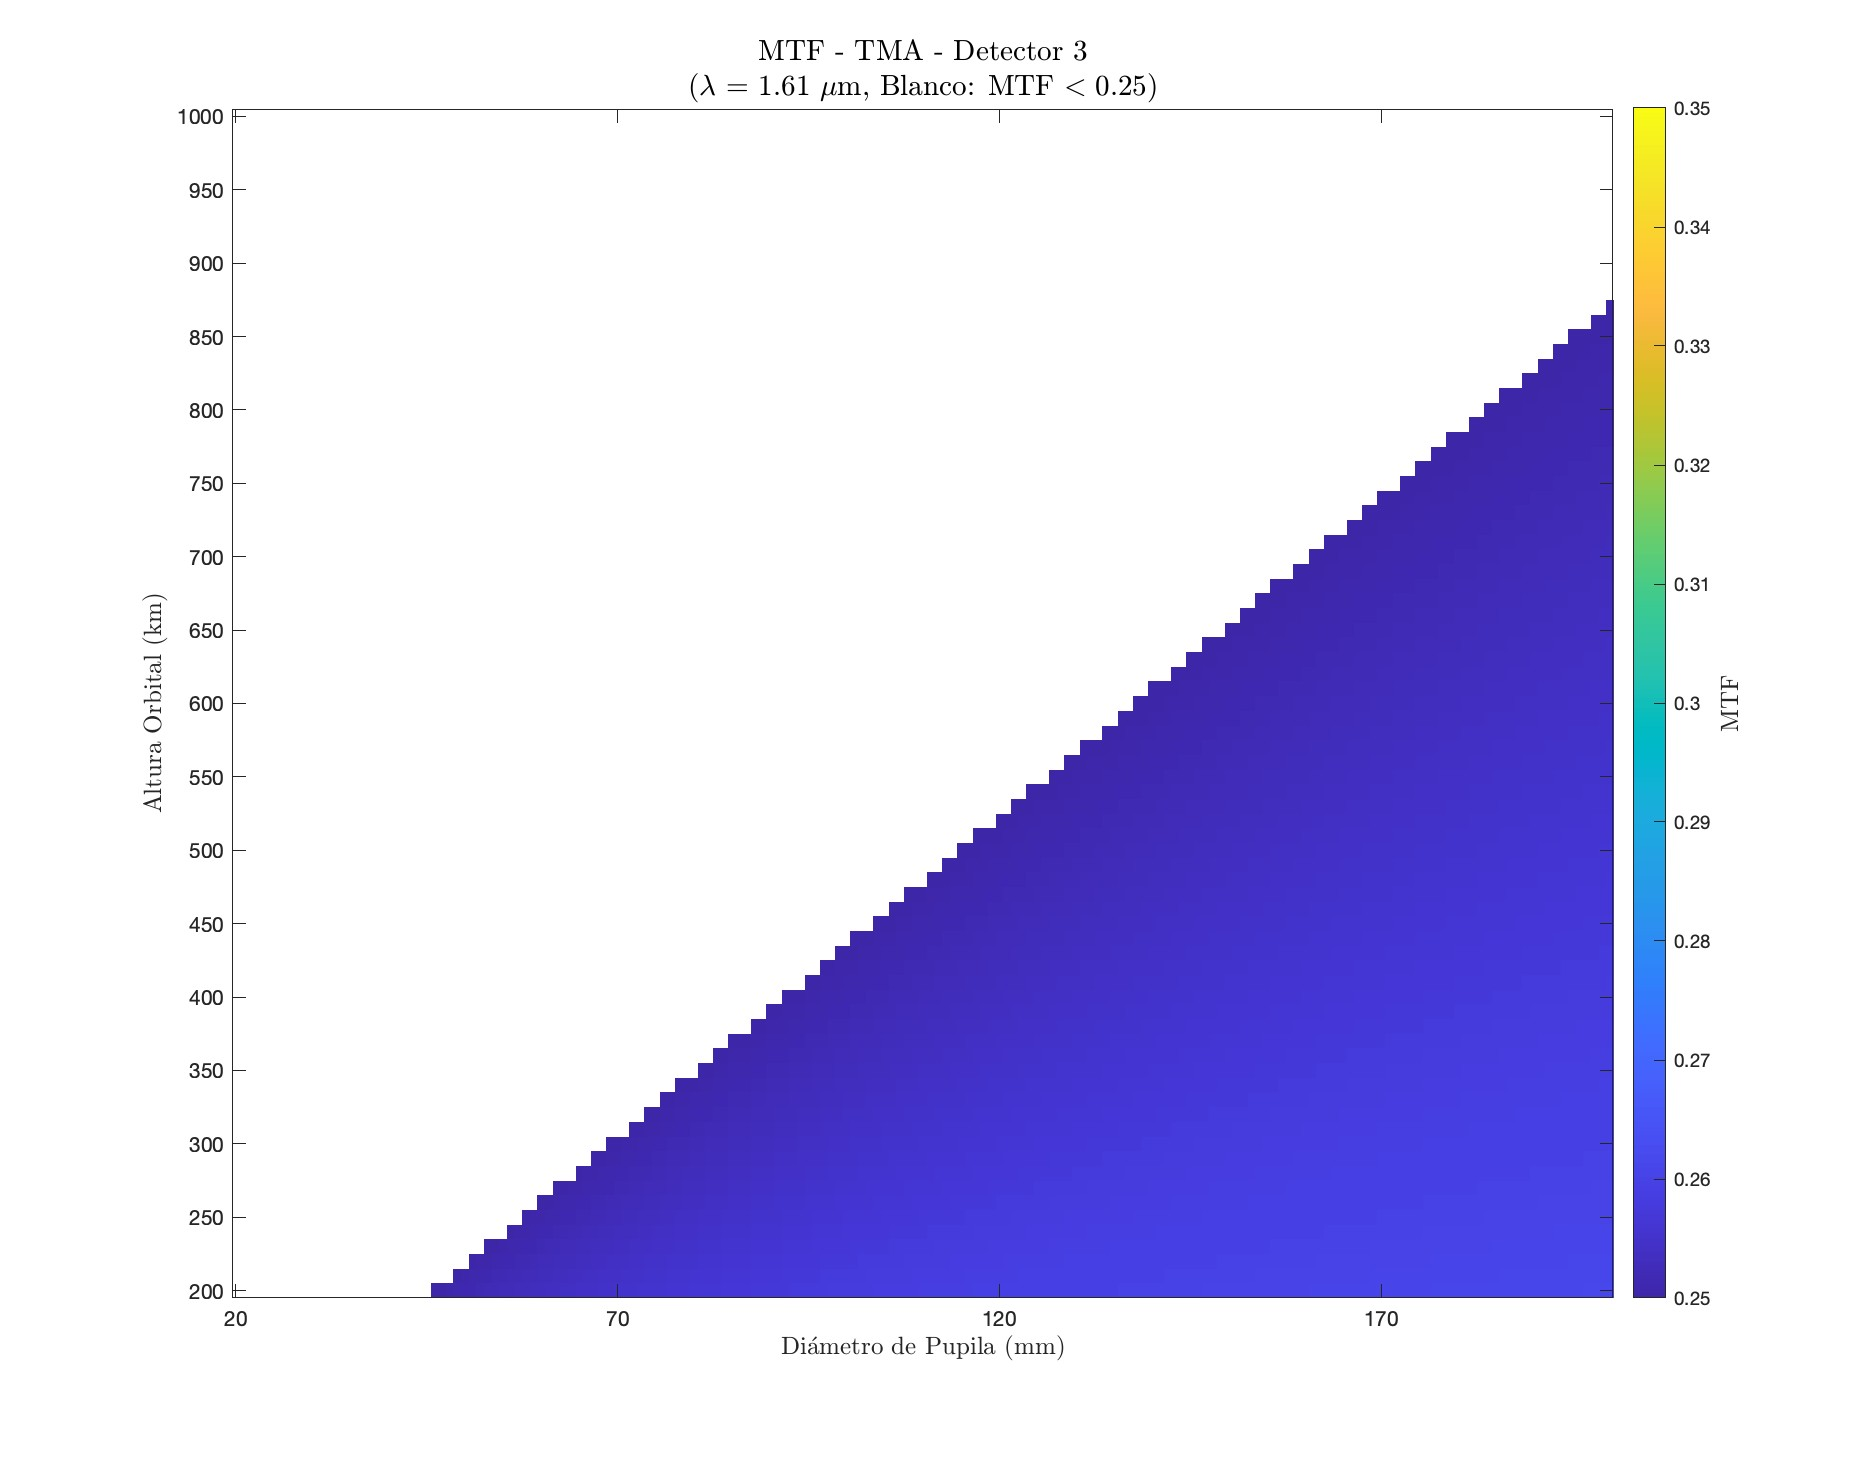
\includegraphics[width=0.48\linewidth]{4.Payload/MTF/MTF_Lambda1_Detector3_Telescopio4_heatmap.jpg} \\
\end{tabular}

\caption{Mapas de calor resultantes del calculo de MTF: Banda 1,61 \textmu m; Detector 3}
\end{figure}
\end{landscape}




%% LAMBDA 2 %%
%========================================================================================
%% DETECTOR 1
\begin{landscape}
\begin{figure}[p]
\centering
\setlength{\tabcolsep}{2pt}
\renewcommand{\arraystretch}{0}
\paragraph{Banda $2,01\ \mu m$}
\begin{tabular}{cc}
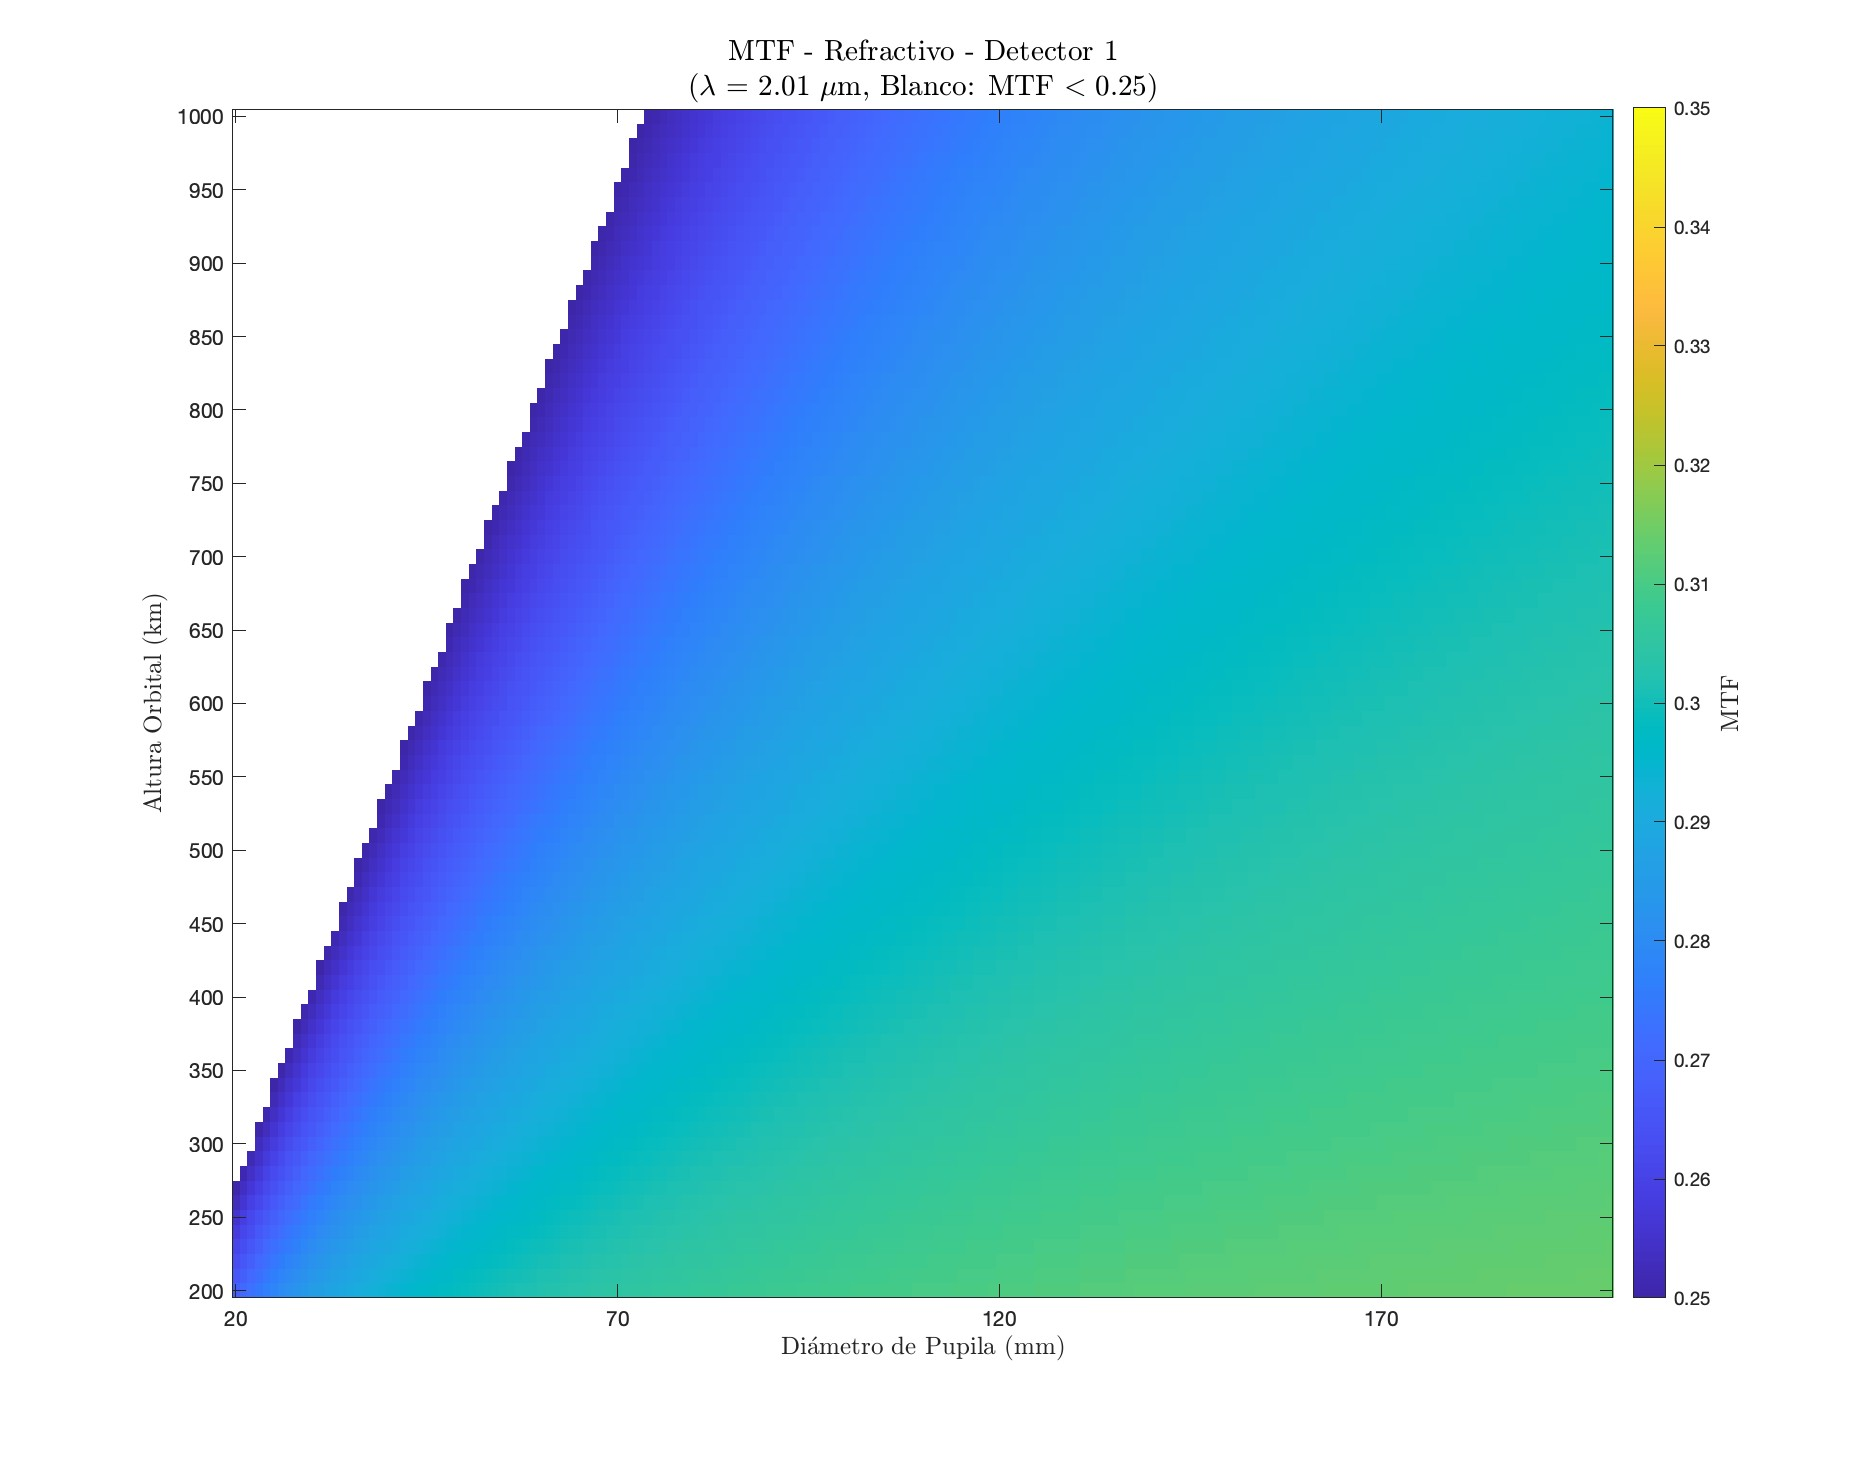
\includegraphics[width=0.48\linewidth]{4.Payload/MTF/MTF_Lambda2_Detector1_Telescopio1_heatmap.jpg} &
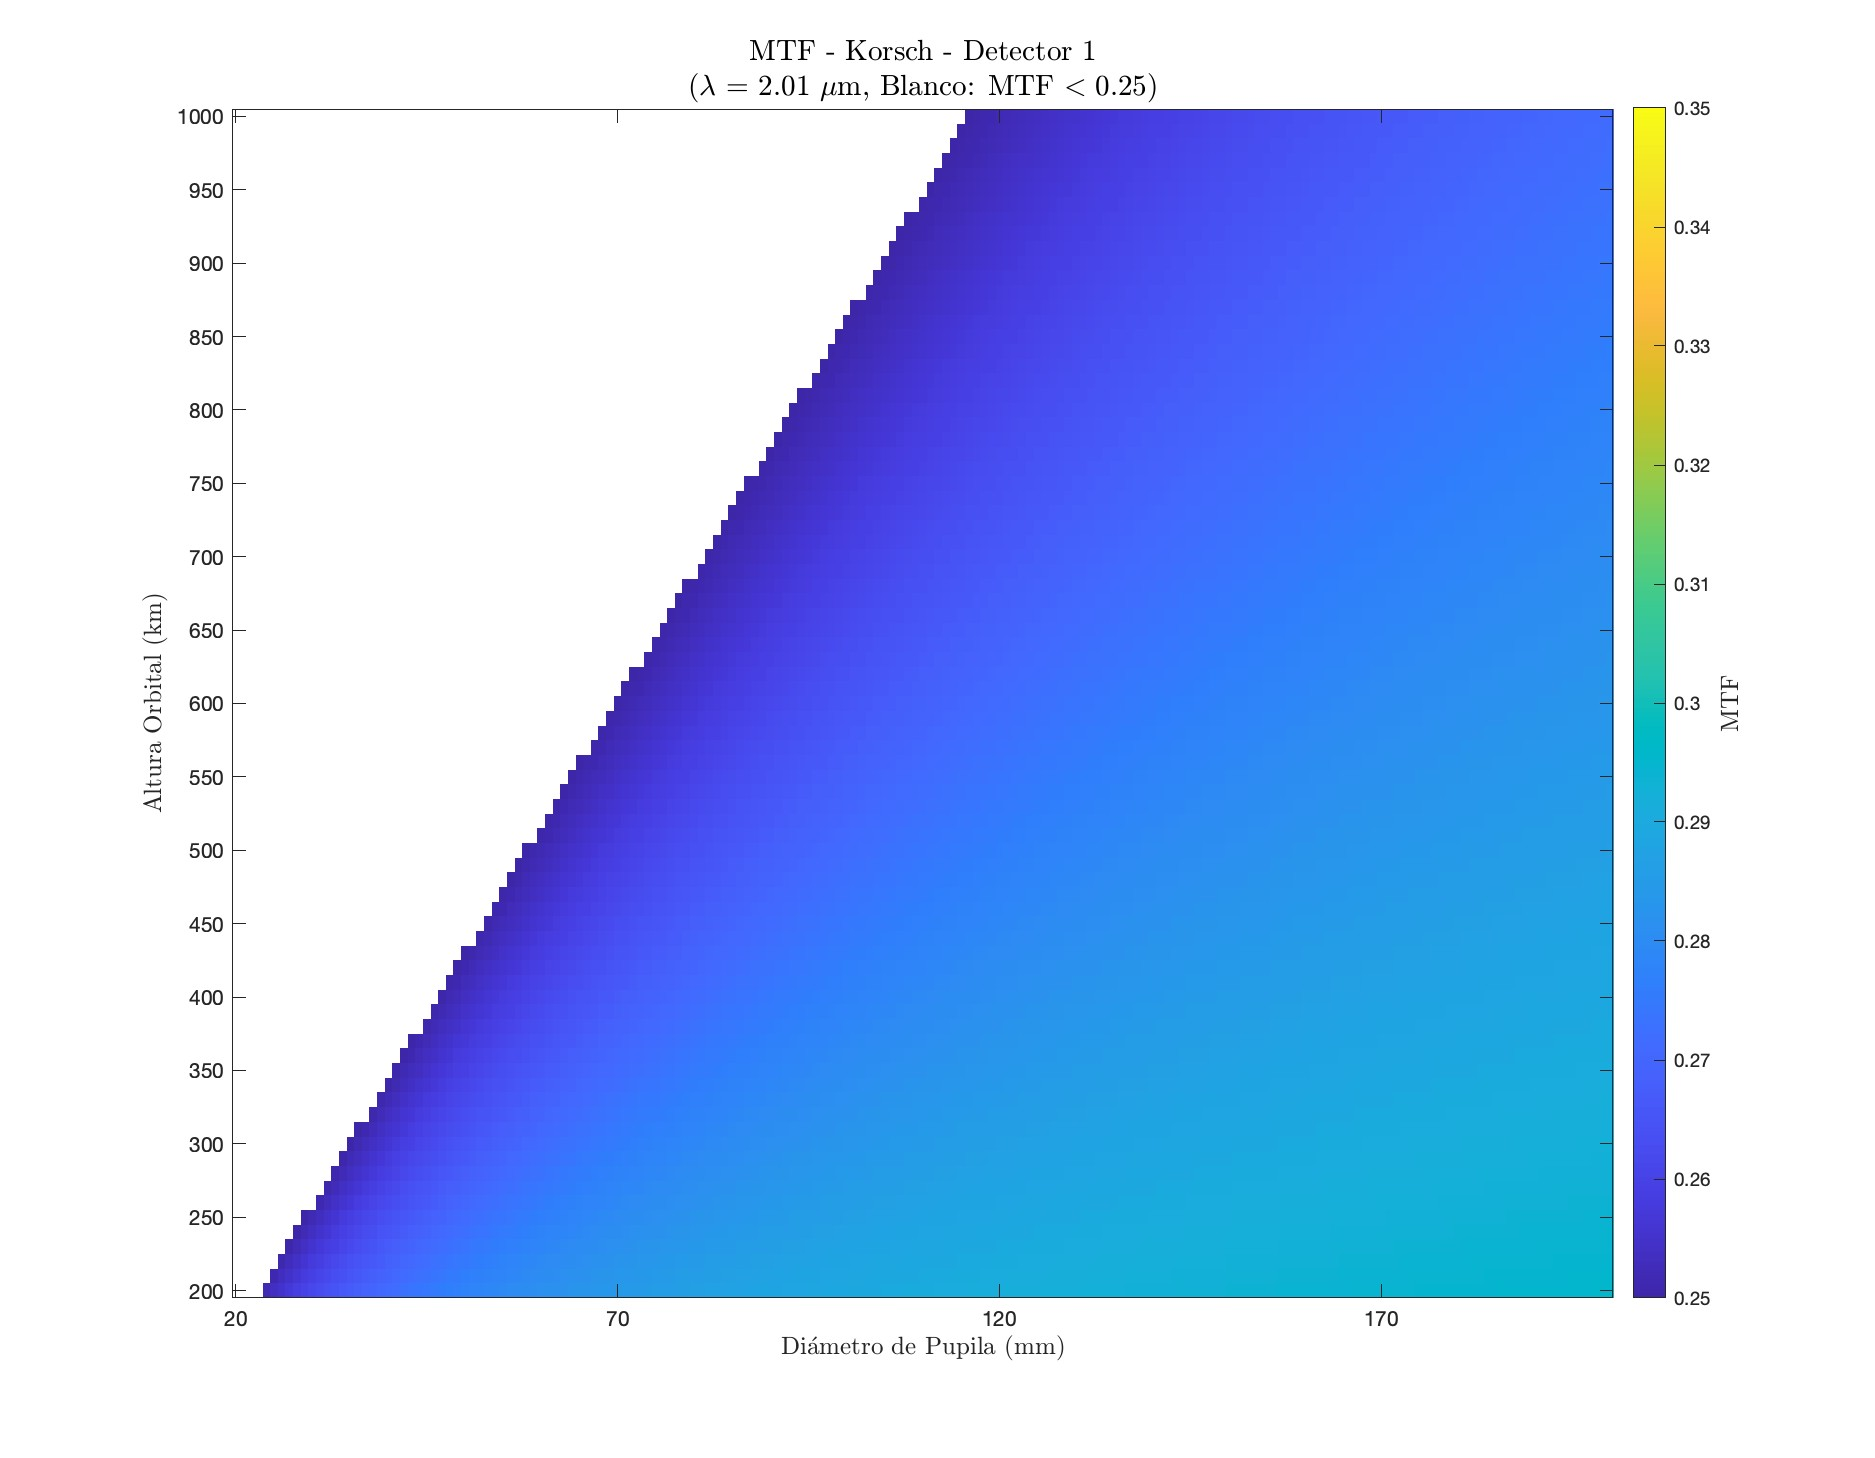
\includegraphics[width=0.48\linewidth]{4.Payload/MTF/MTF_Lambda2_Detector1_Telescopio2_heatmap.jpg} \\
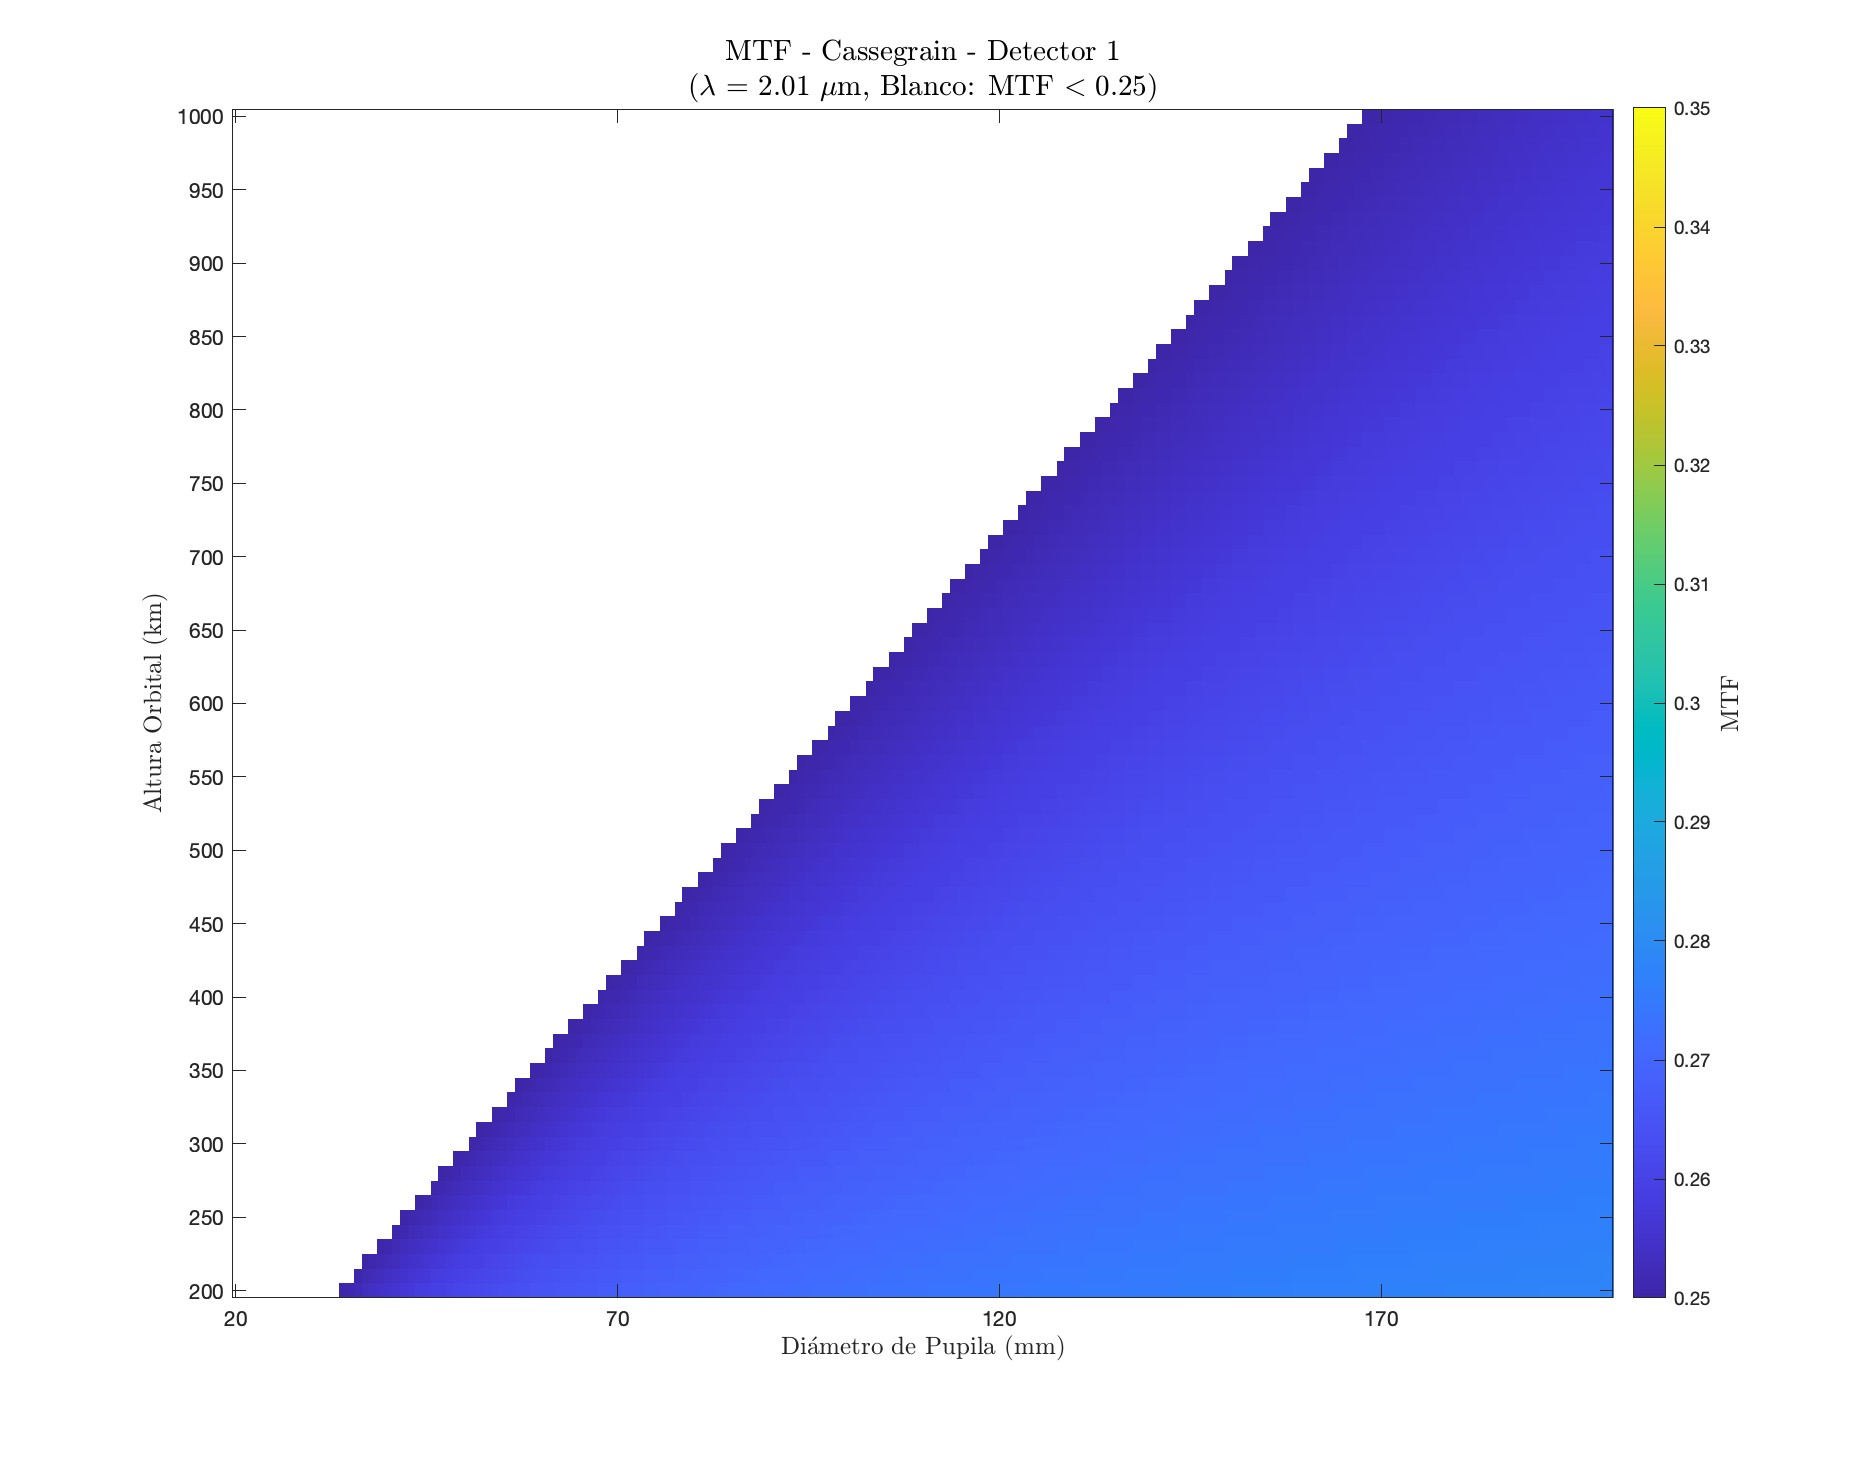
\includegraphics[width=0.48\linewidth]{4.Payload/MTF/MTF_Lambda2_Detector1_Telescopio3_heatmap.jpg} &
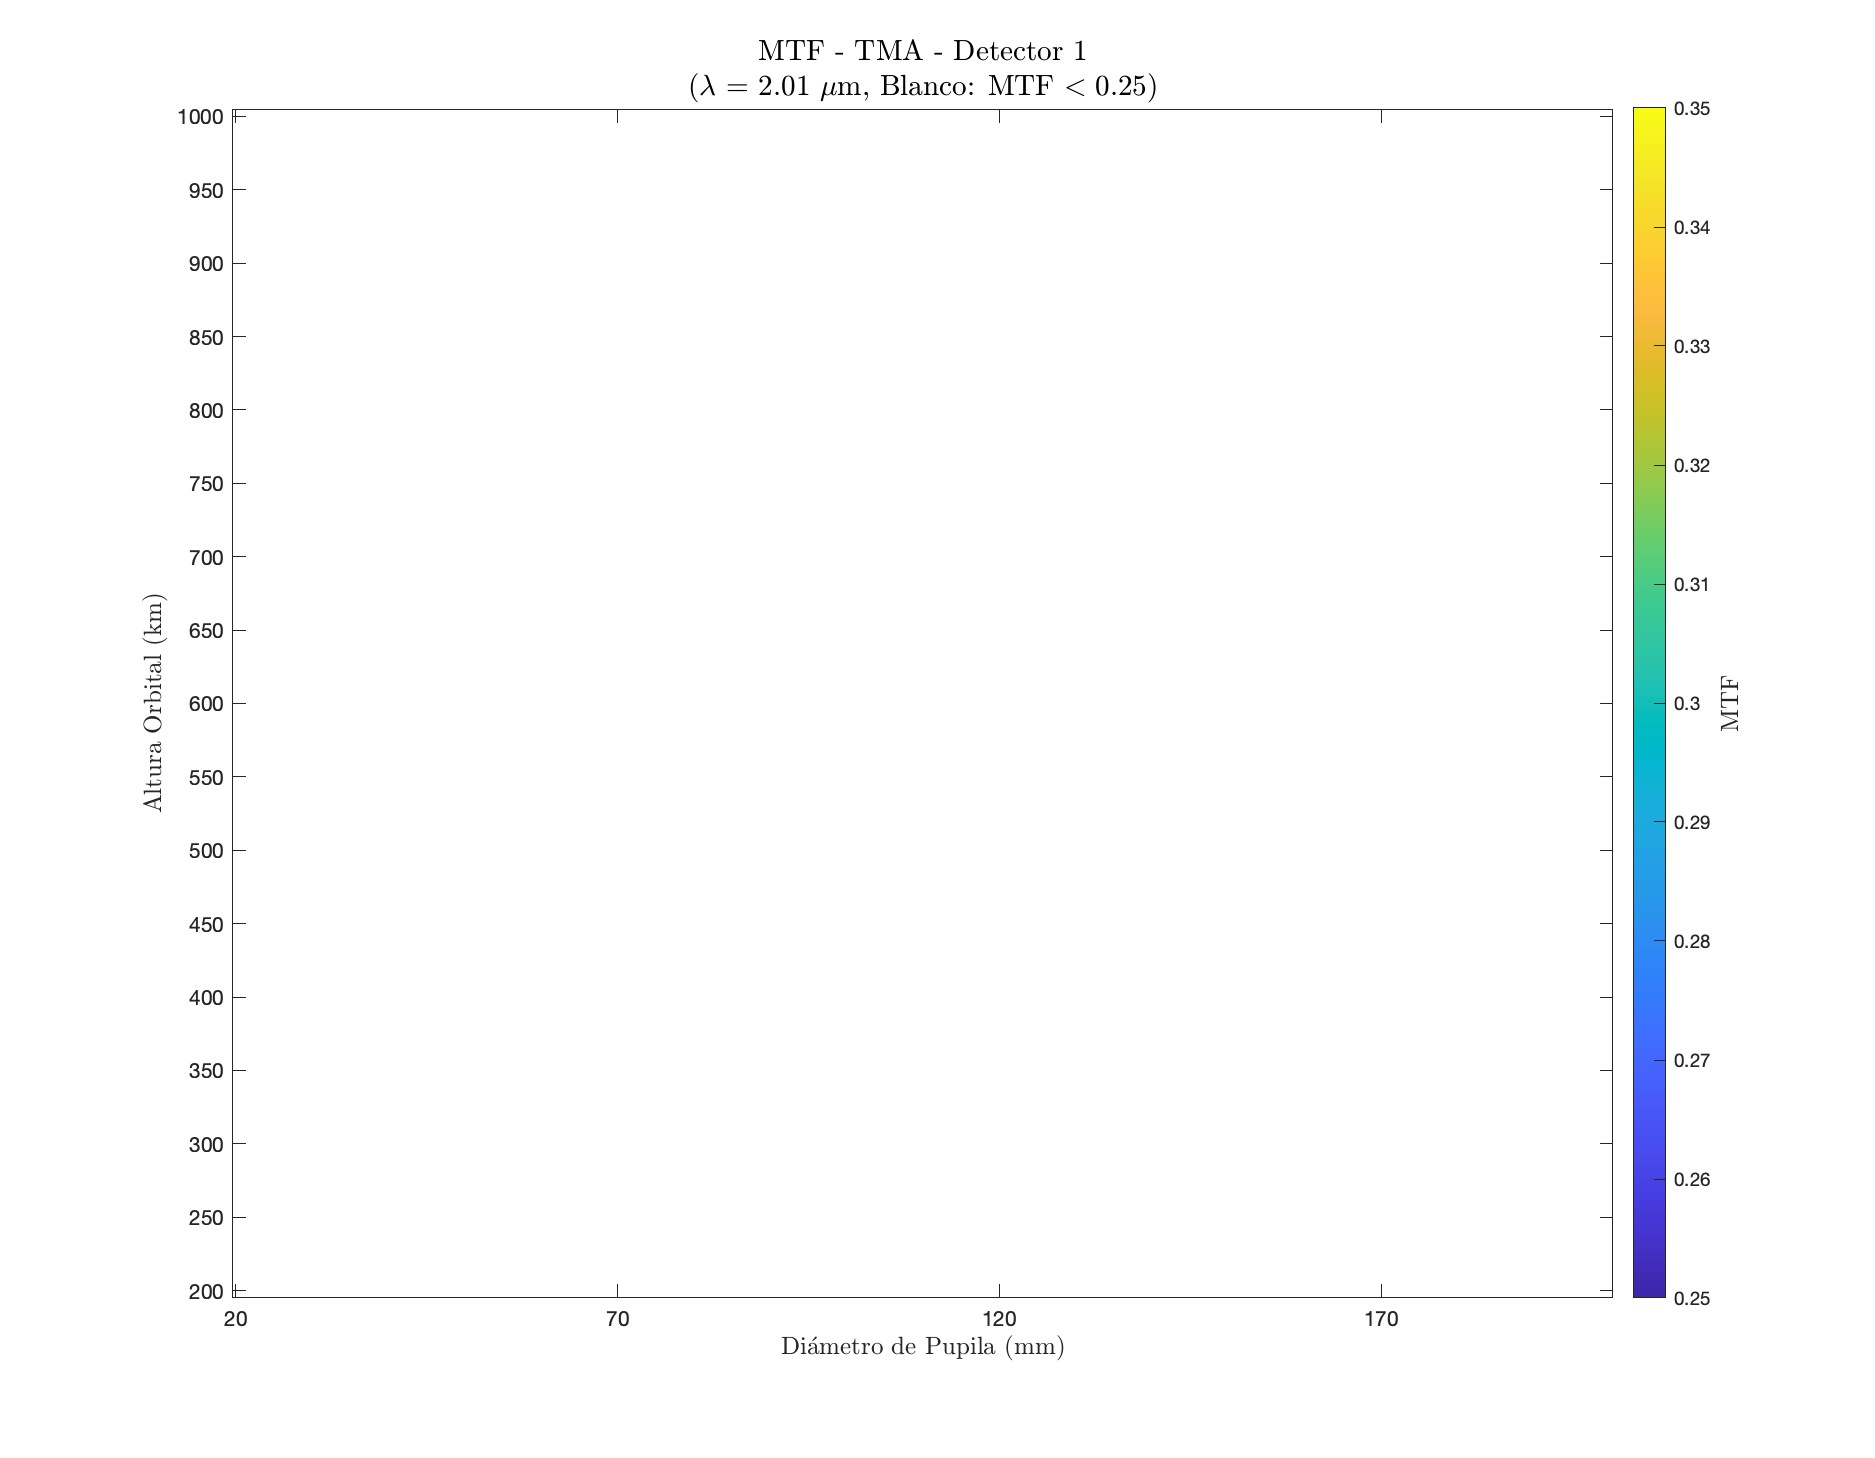
\includegraphics[width=0.48\linewidth]{4.Payload/MTF/MTF_Lambda2_Detector1_Telescopio4_heatmap.jpg} \\
\end{tabular}
\caption{Mapas de calor resultantes del calculo de MTF: Banda 2,01 \textmu m; Detector 1}
\end{figure}
\end{landscape}


%% DETECTOR 2
\begin{landscape}
\begin{figure}[p]
\centering
\setlength{\tabcolsep}{2pt}
\renewcommand{\arraystretch}{0}

\begin{tabular}{cc}
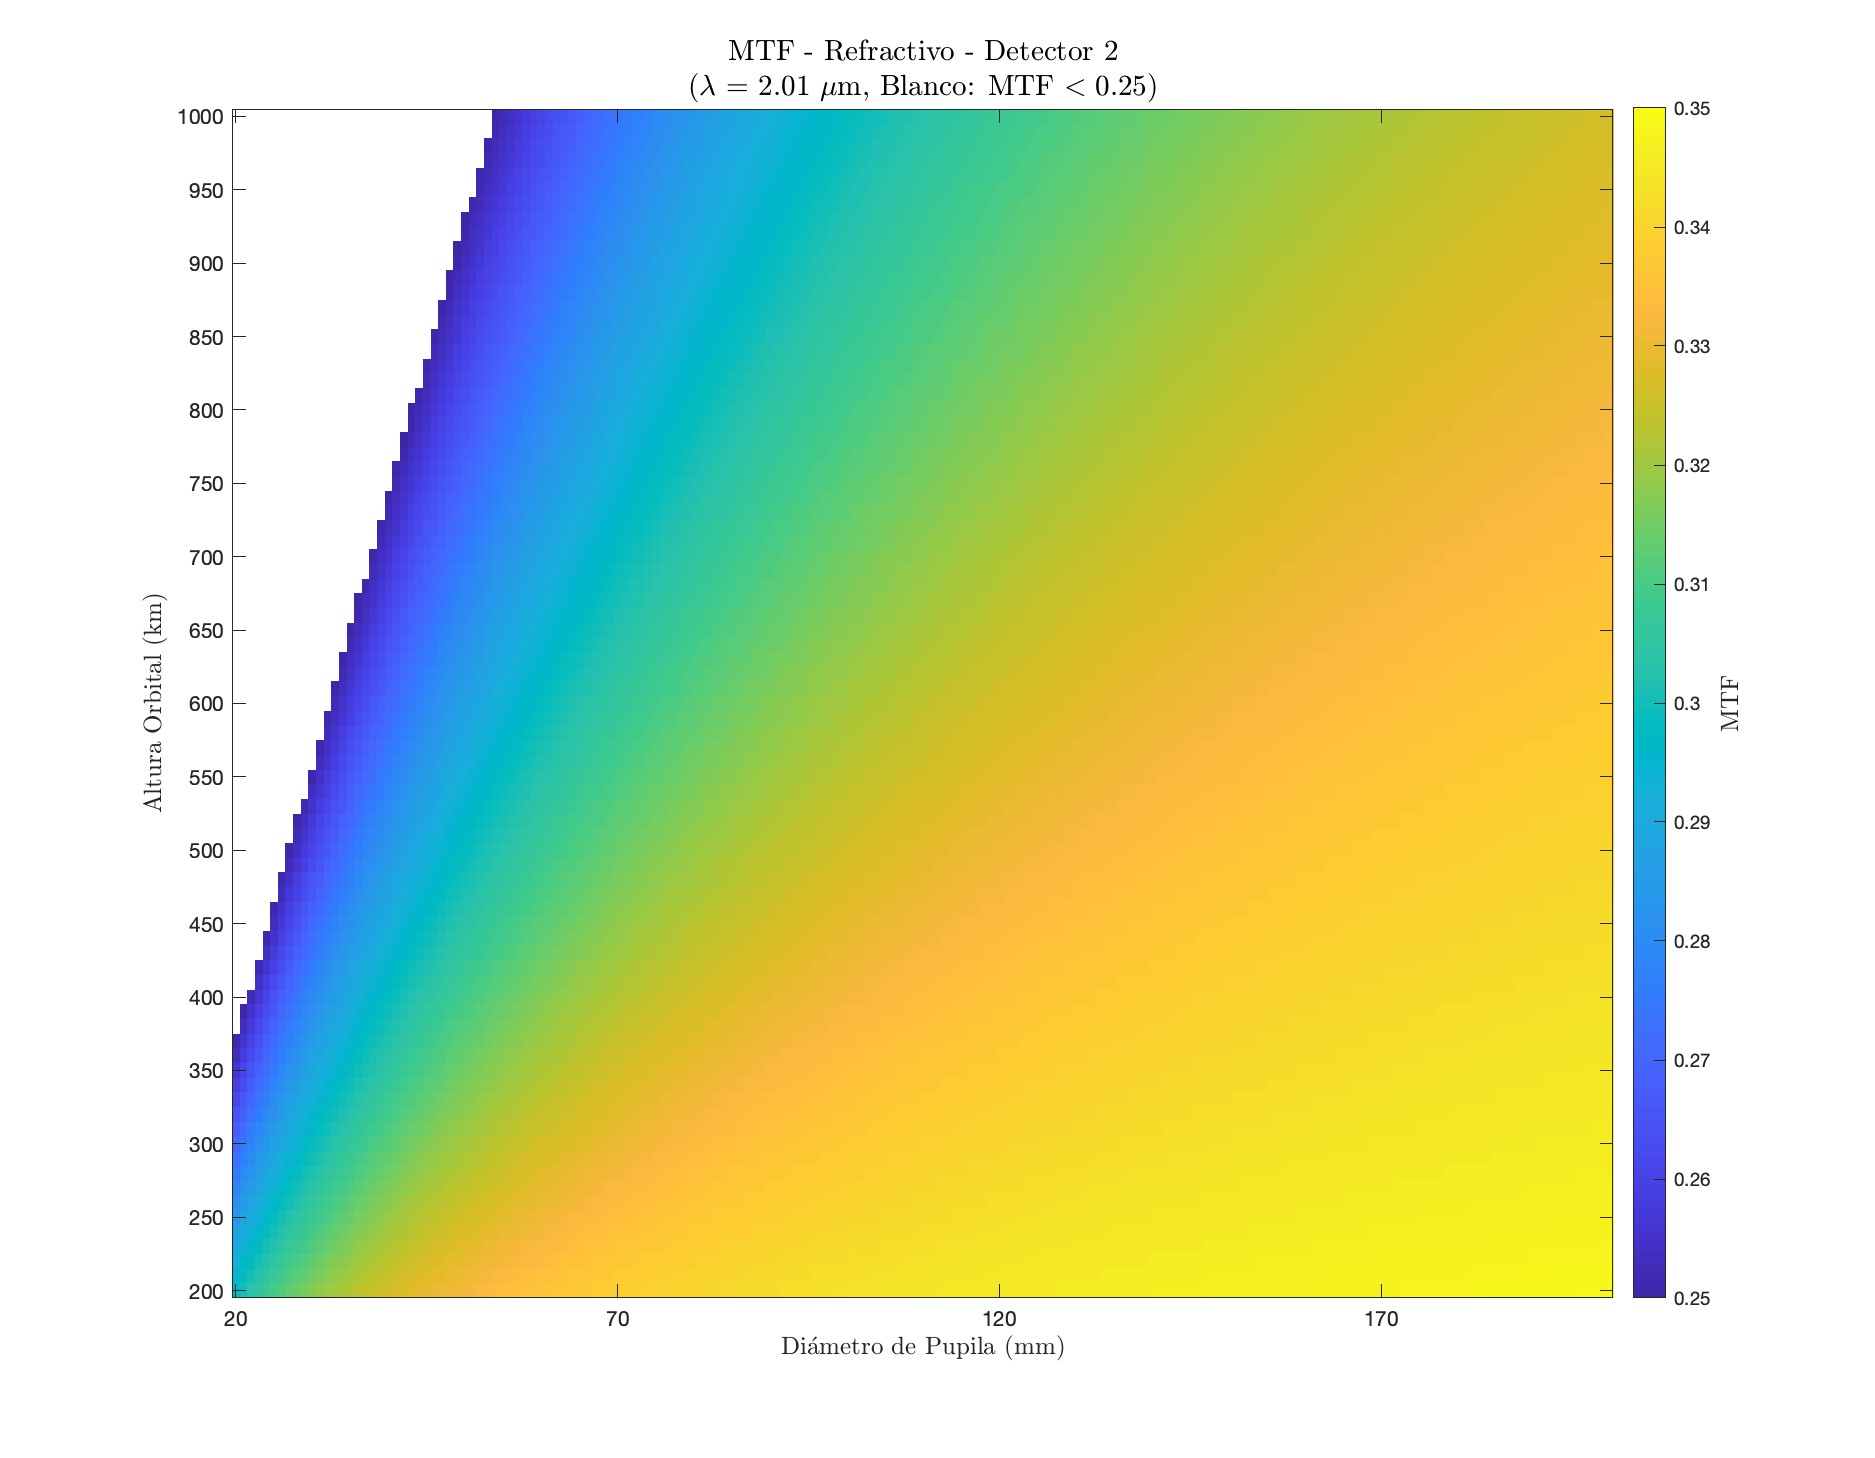
\includegraphics[width=0.48\linewidth]{4.Payload/MTF/MTF_Lambda2_Detector2_Telescopio1_heatmap.jpg} &
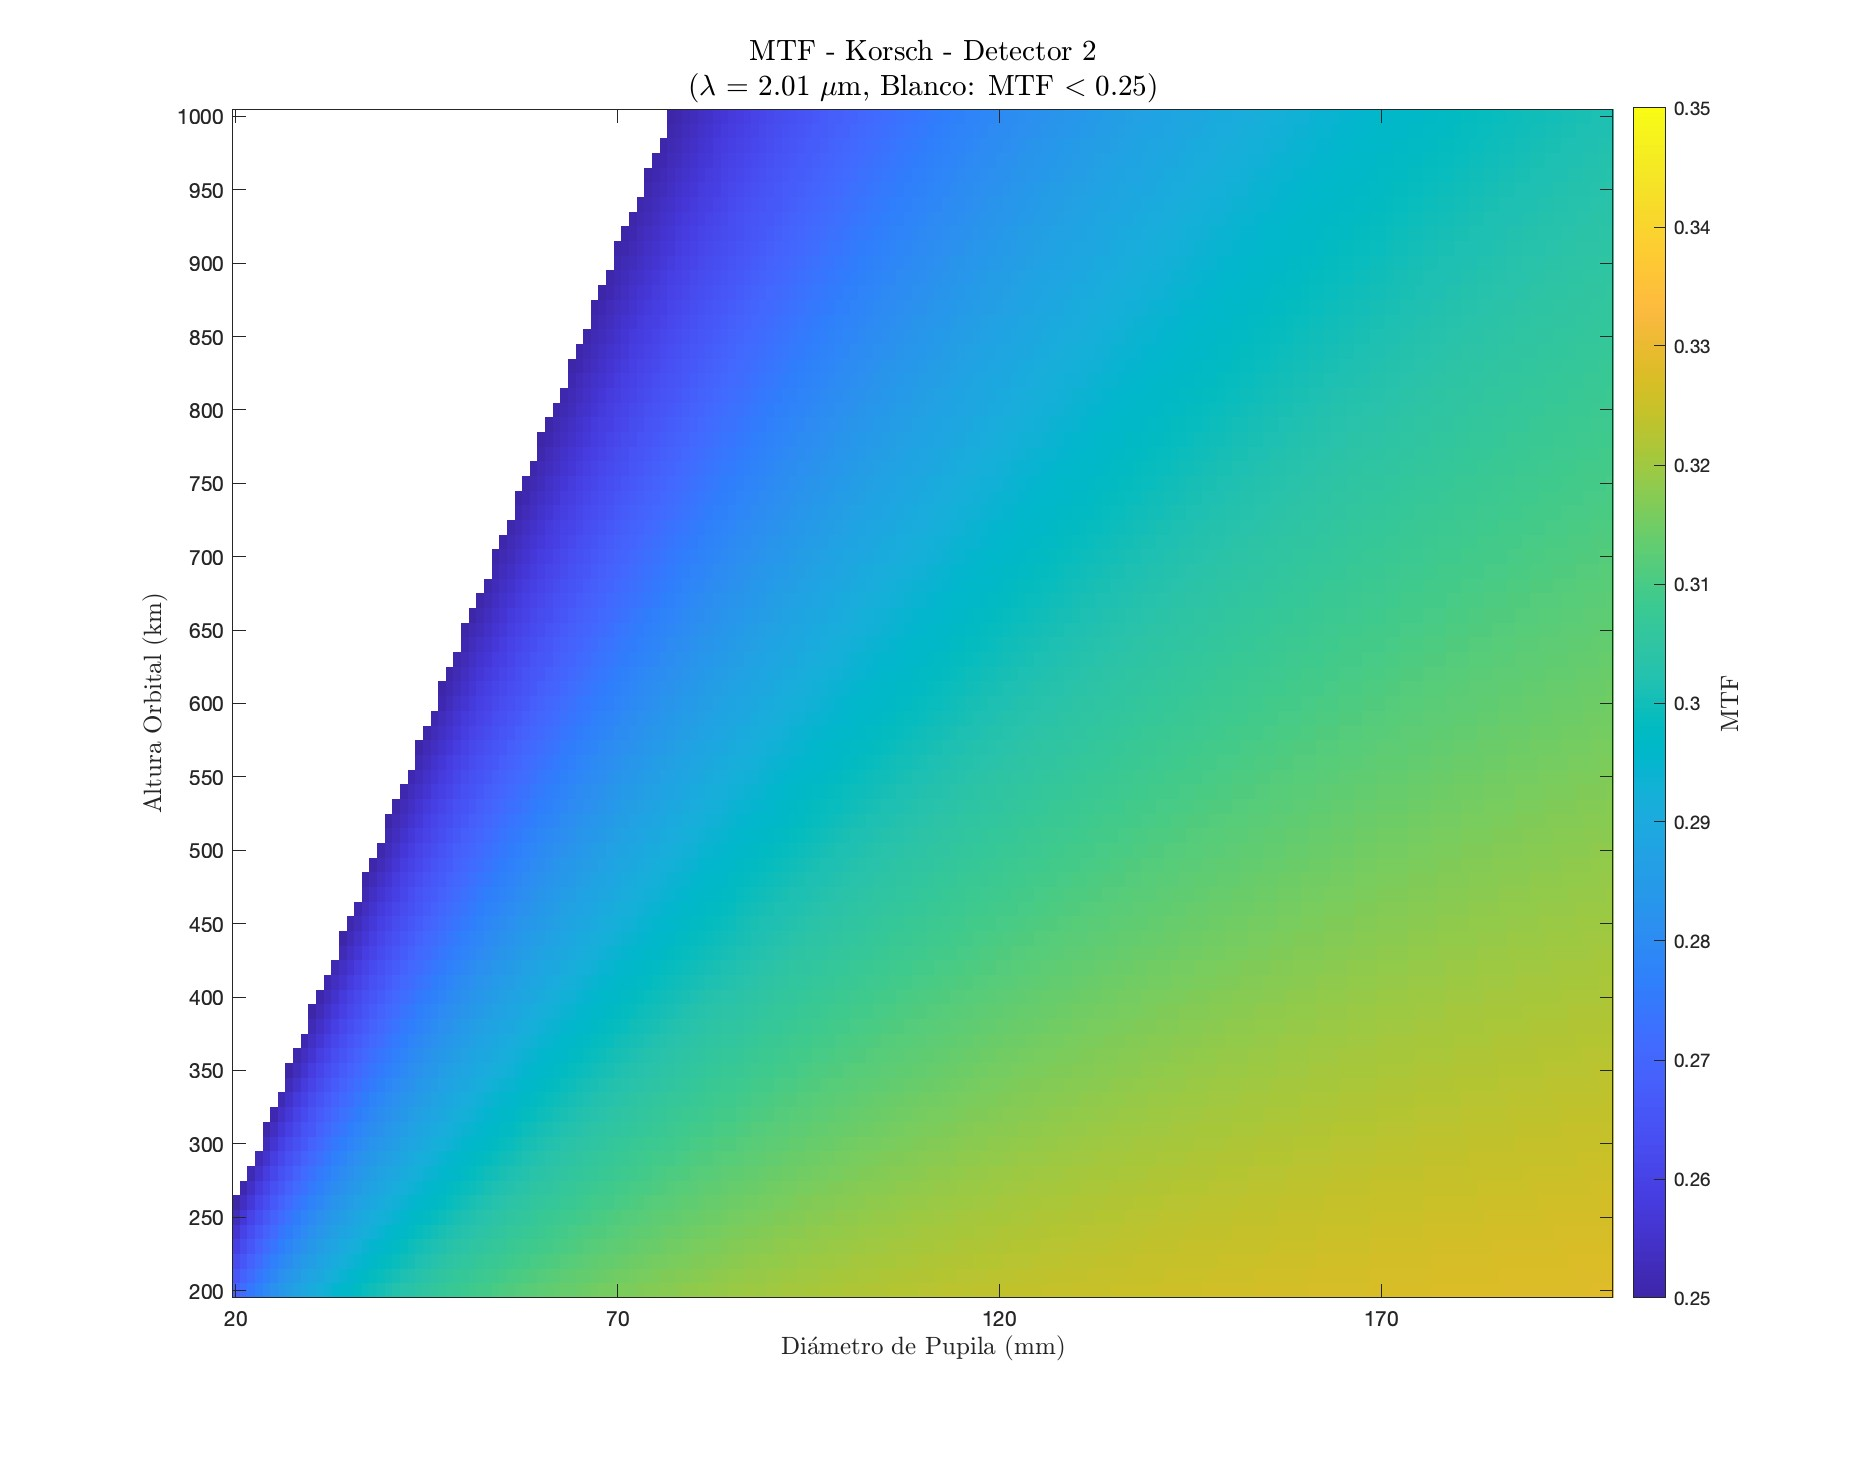
\includegraphics[width=0.48\linewidth]{4.Payload/MTF/MTF_Lambda2_Detector2_Telescopio2_heatmap.jpg} \\
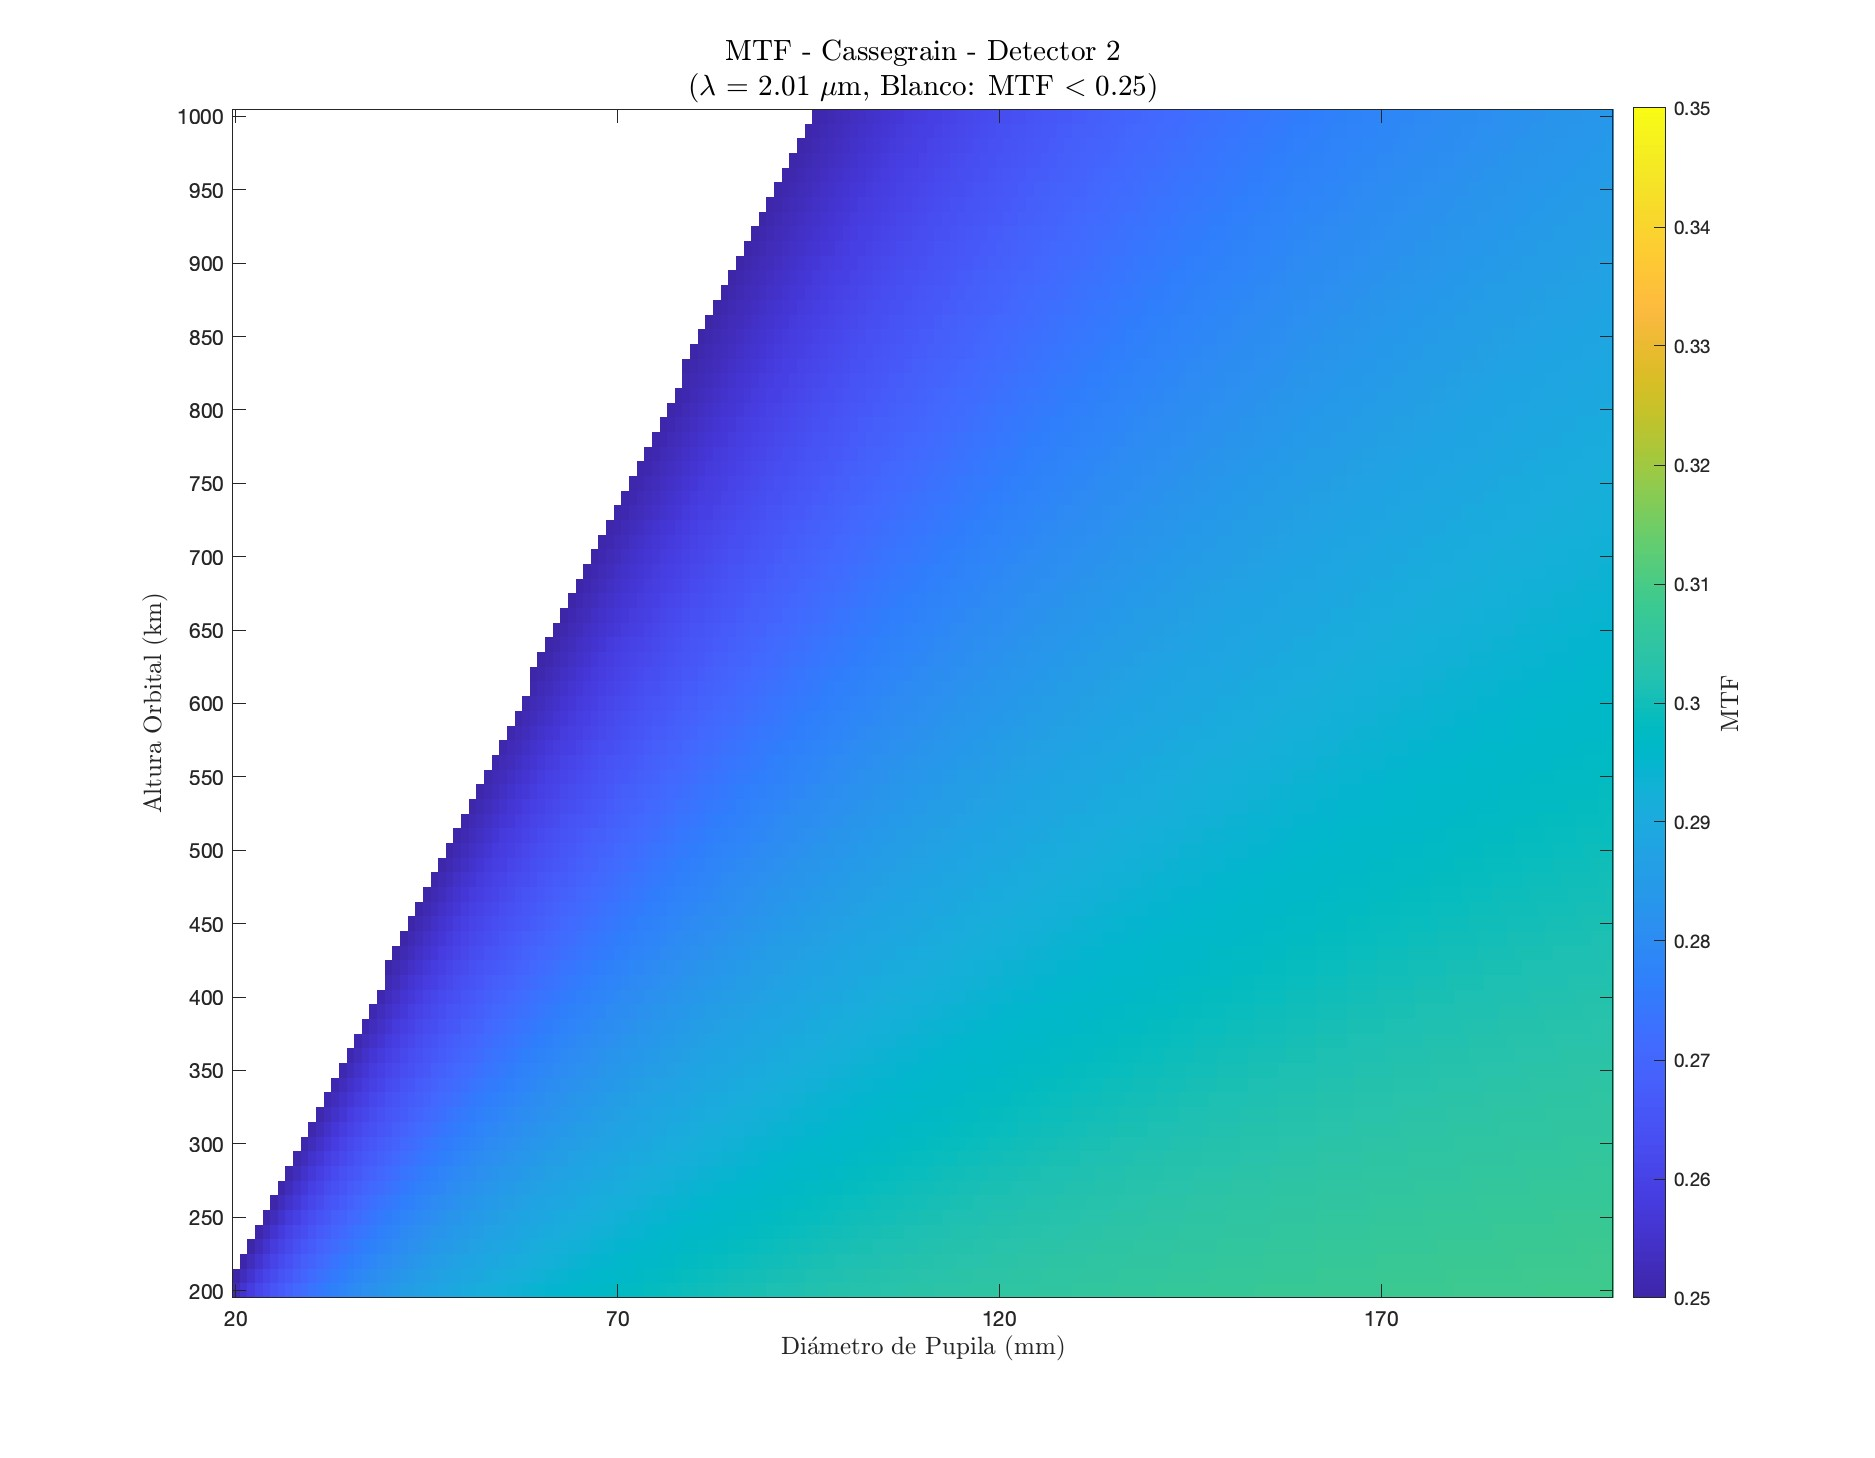
\includegraphics[width=0.48\linewidth]{4.Payload/MTF/MTF_Lambda2_Detector2_Telescopio3_heatmap.jpg} &
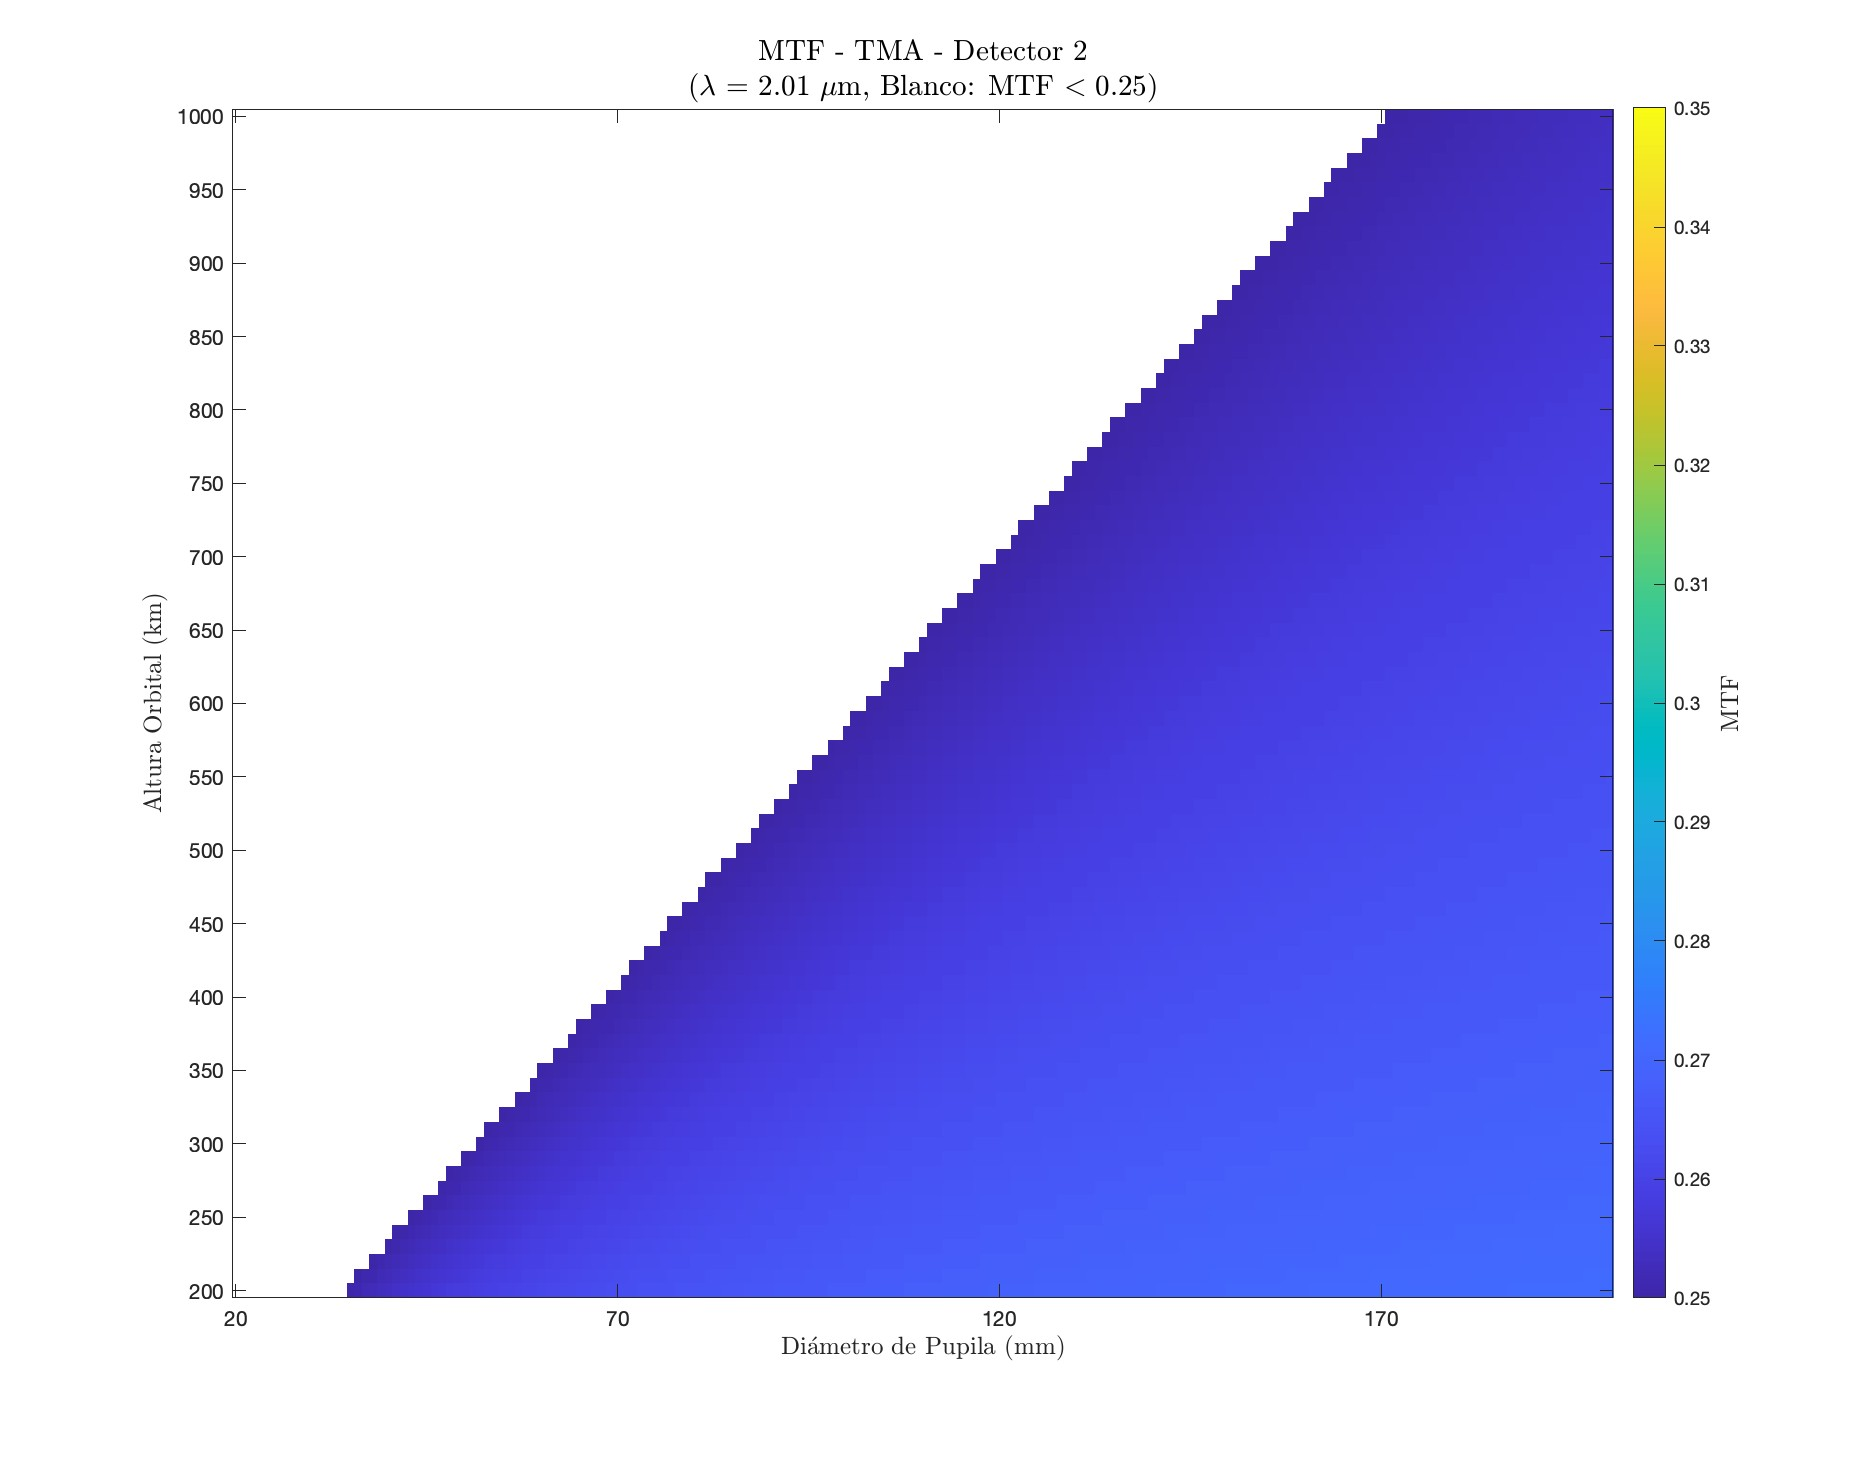
\includegraphics[width=0.48\linewidth]{4.Payload/MTF/MTF_Lambda2_Detector2_Telescopio4_heatmap.jpg} \\
\end{tabular}
\caption{Mapas de calor resultantes del calculo de MTF: Banda 2,01 \textmu m; Detector 2}
\end{figure}
\end{landscape}


%% DETECTOR 3
\begin{landscape}
\begin{figure}[p]
\centering
\setlength{\tabcolsep}{2pt}
\renewcommand{\arraystretch}{0}

\begin{tabular}{cc}
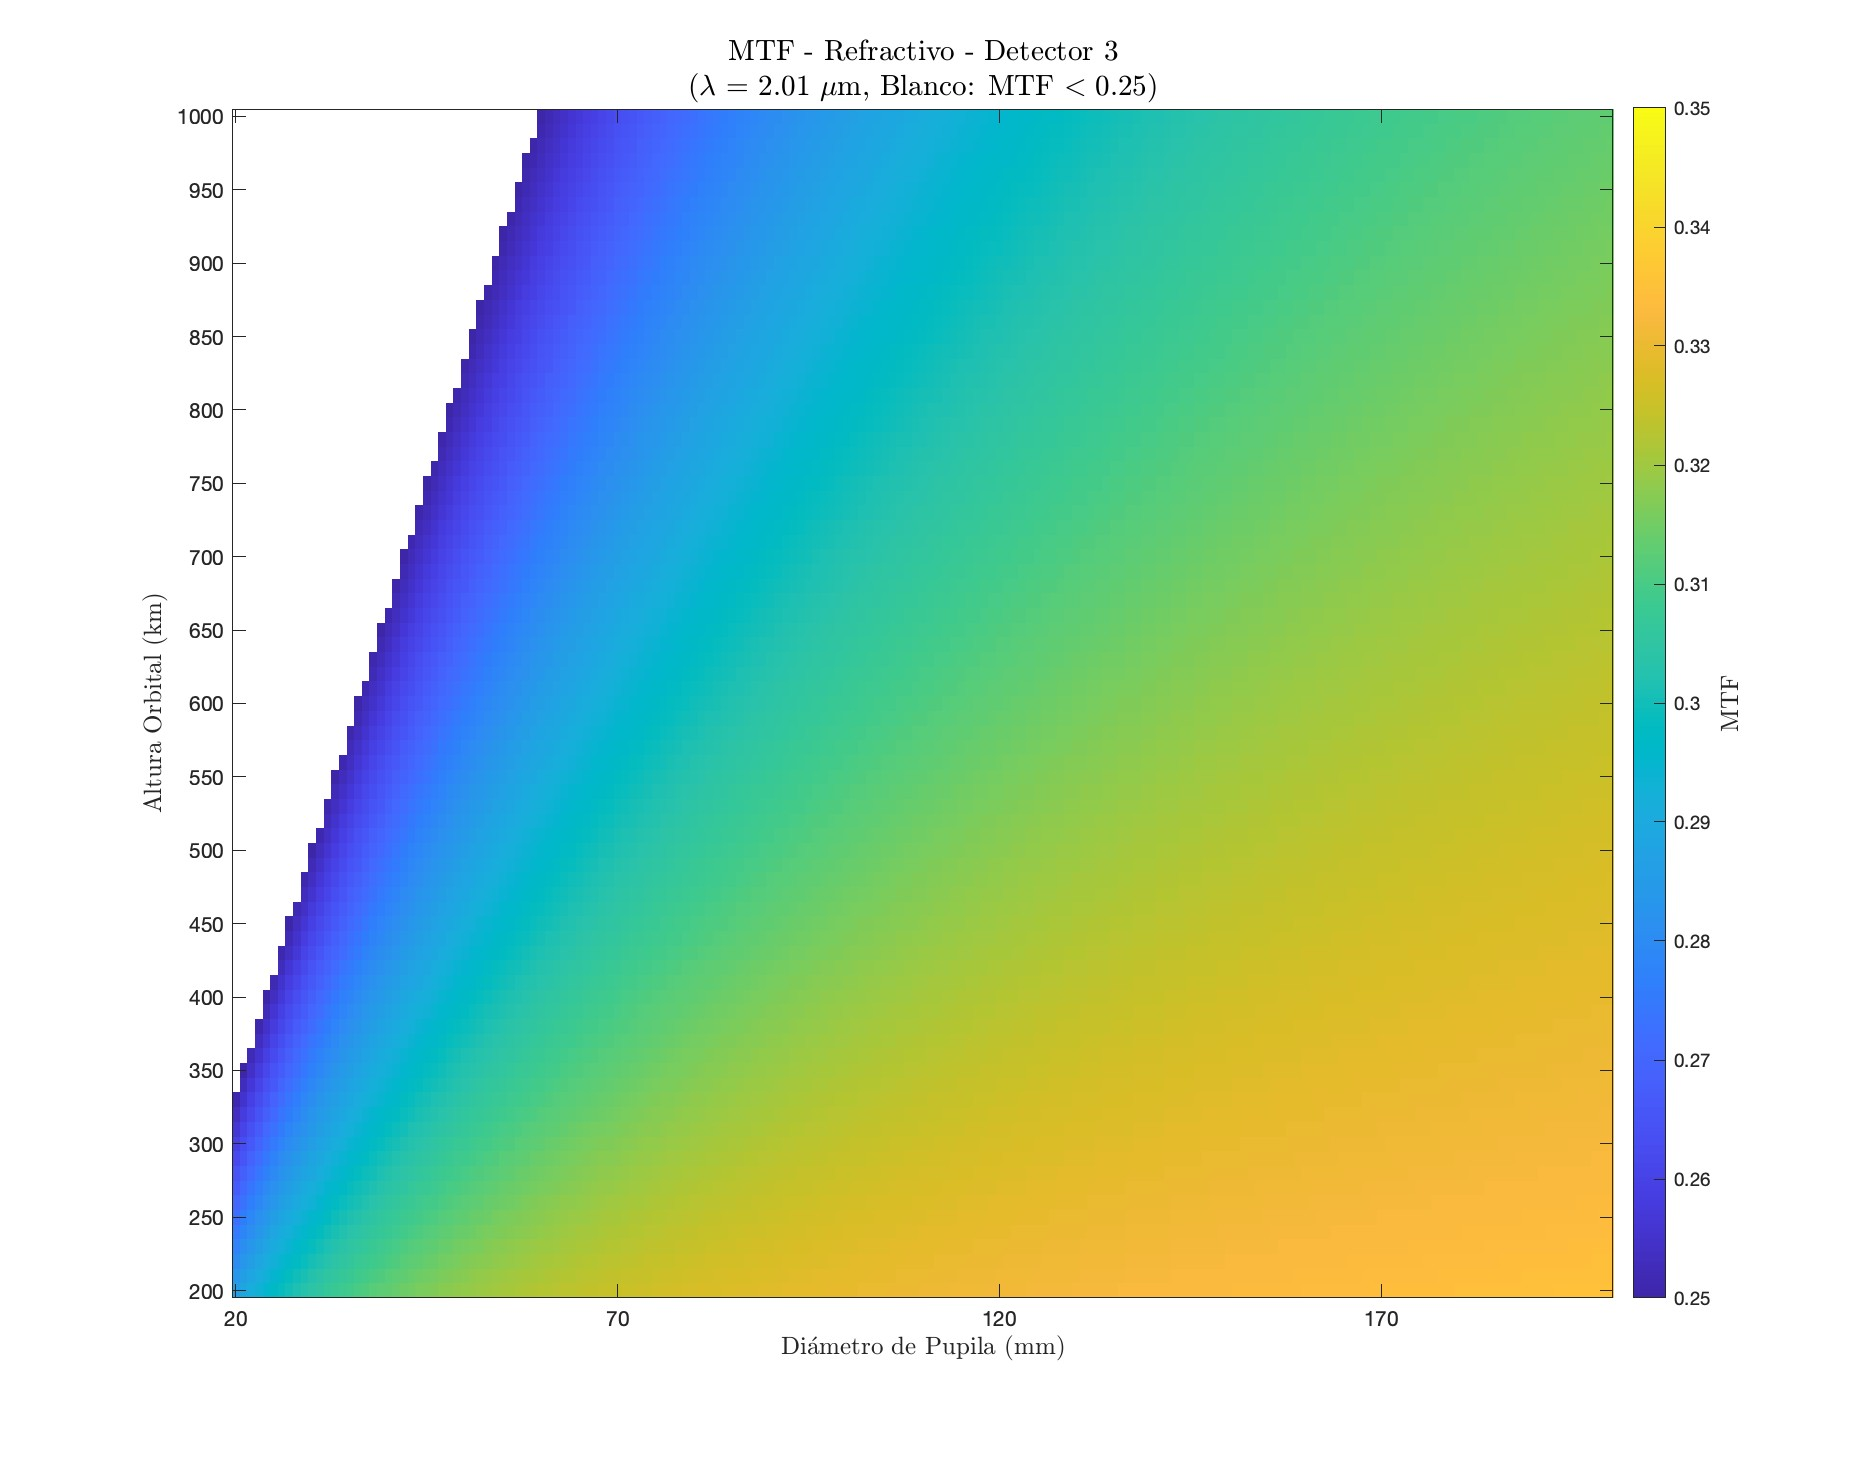
\includegraphics[width=0.48\linewidth]{4.Payload/MTF/MTF_Lambda2_Detector3_Telescopio1_heatmap.jpg} &
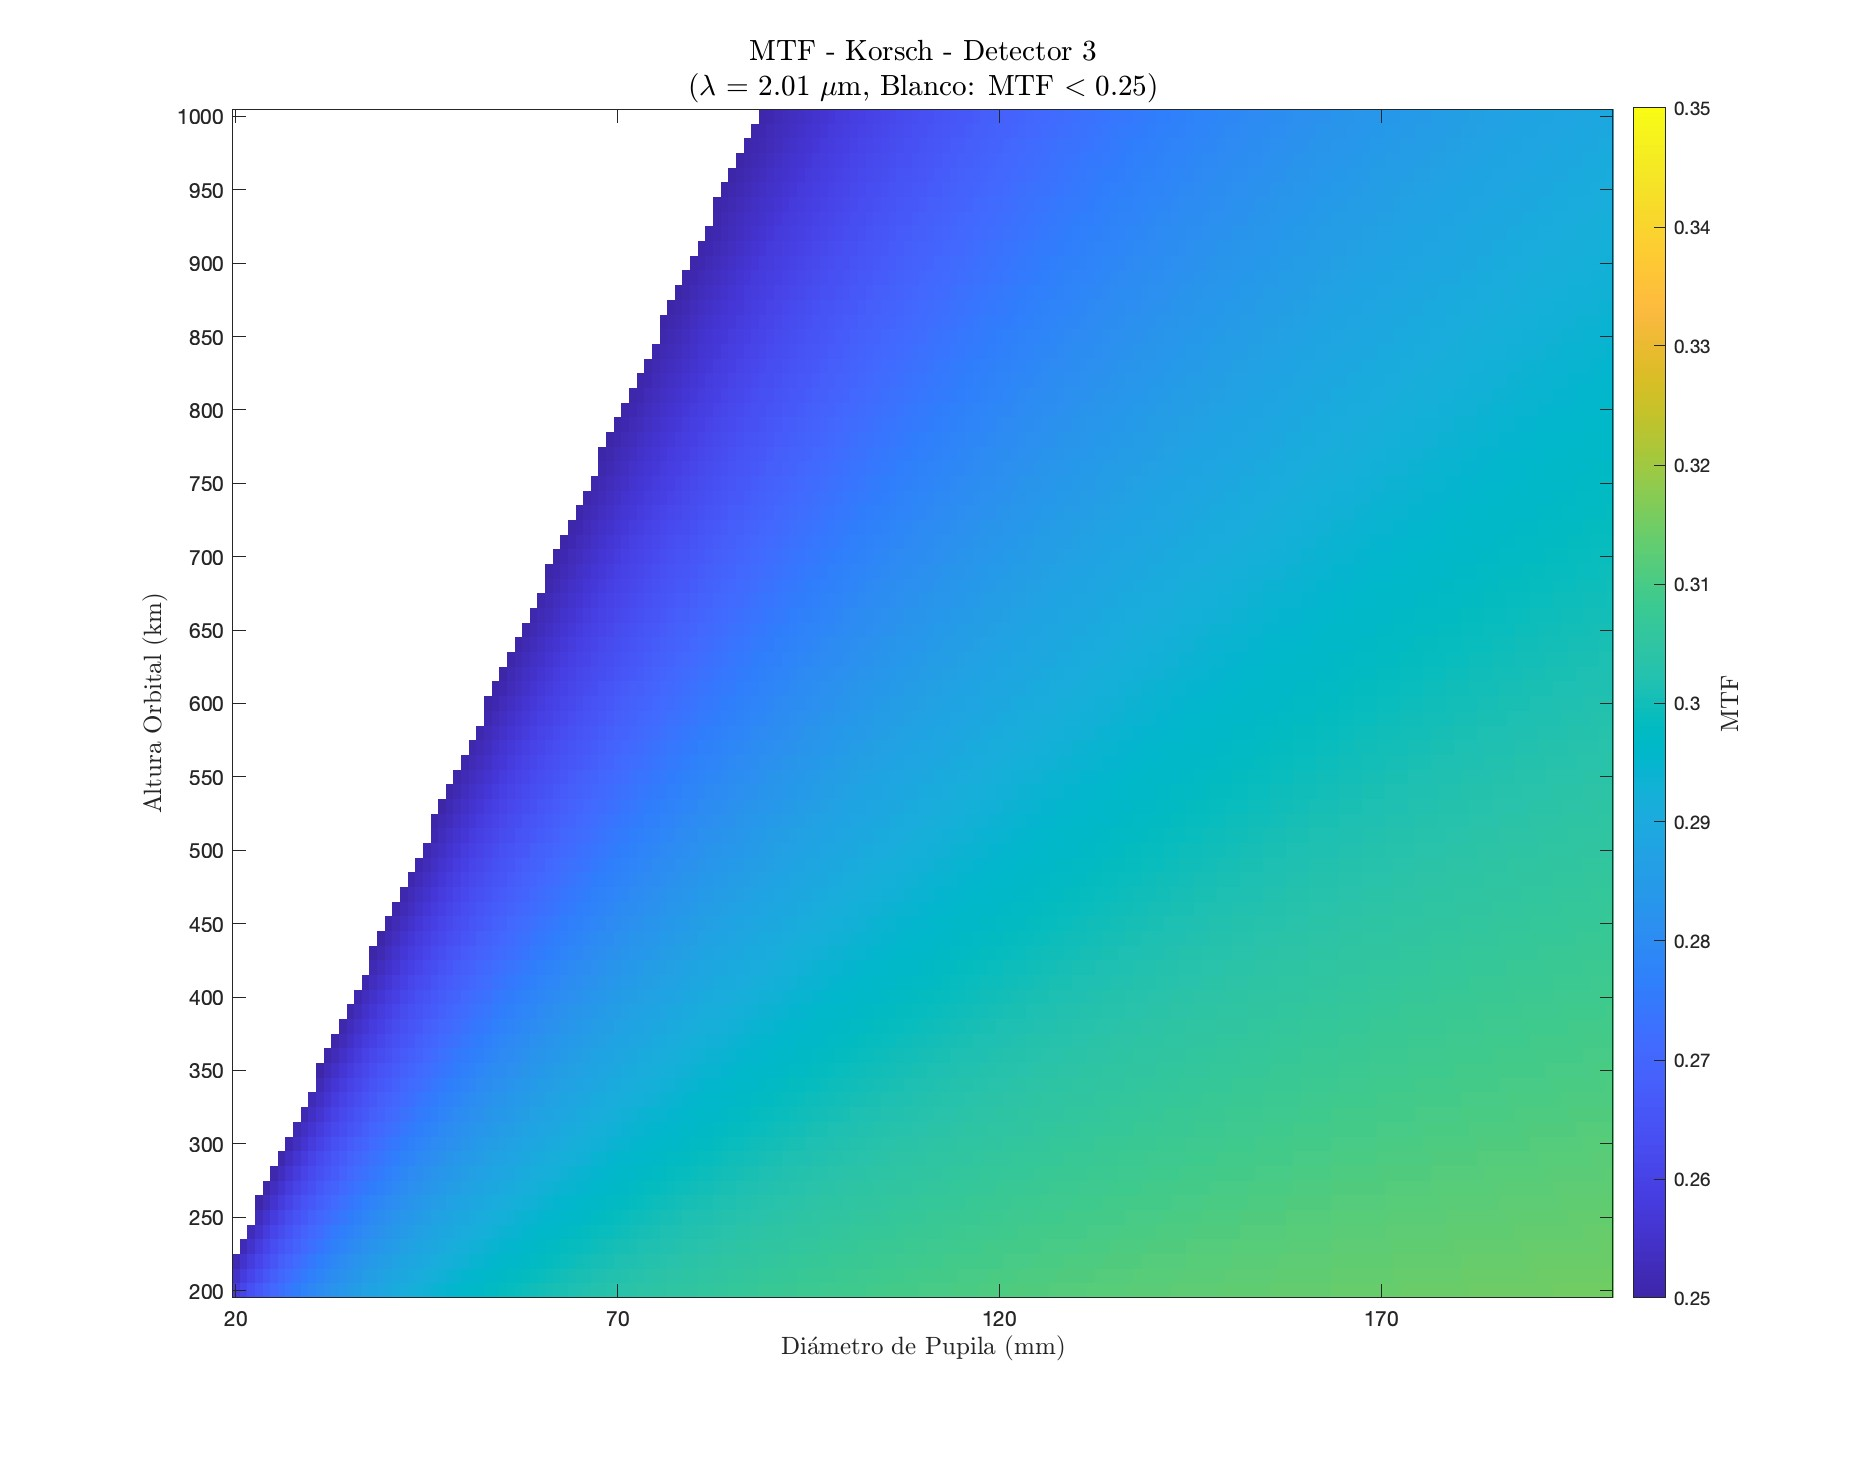
\includegraphics[width=0.48\linewidth]{4.Payload/MTF/MTF_Lambda2_Detector3_Telescopio2_heatmap.jpg} \\
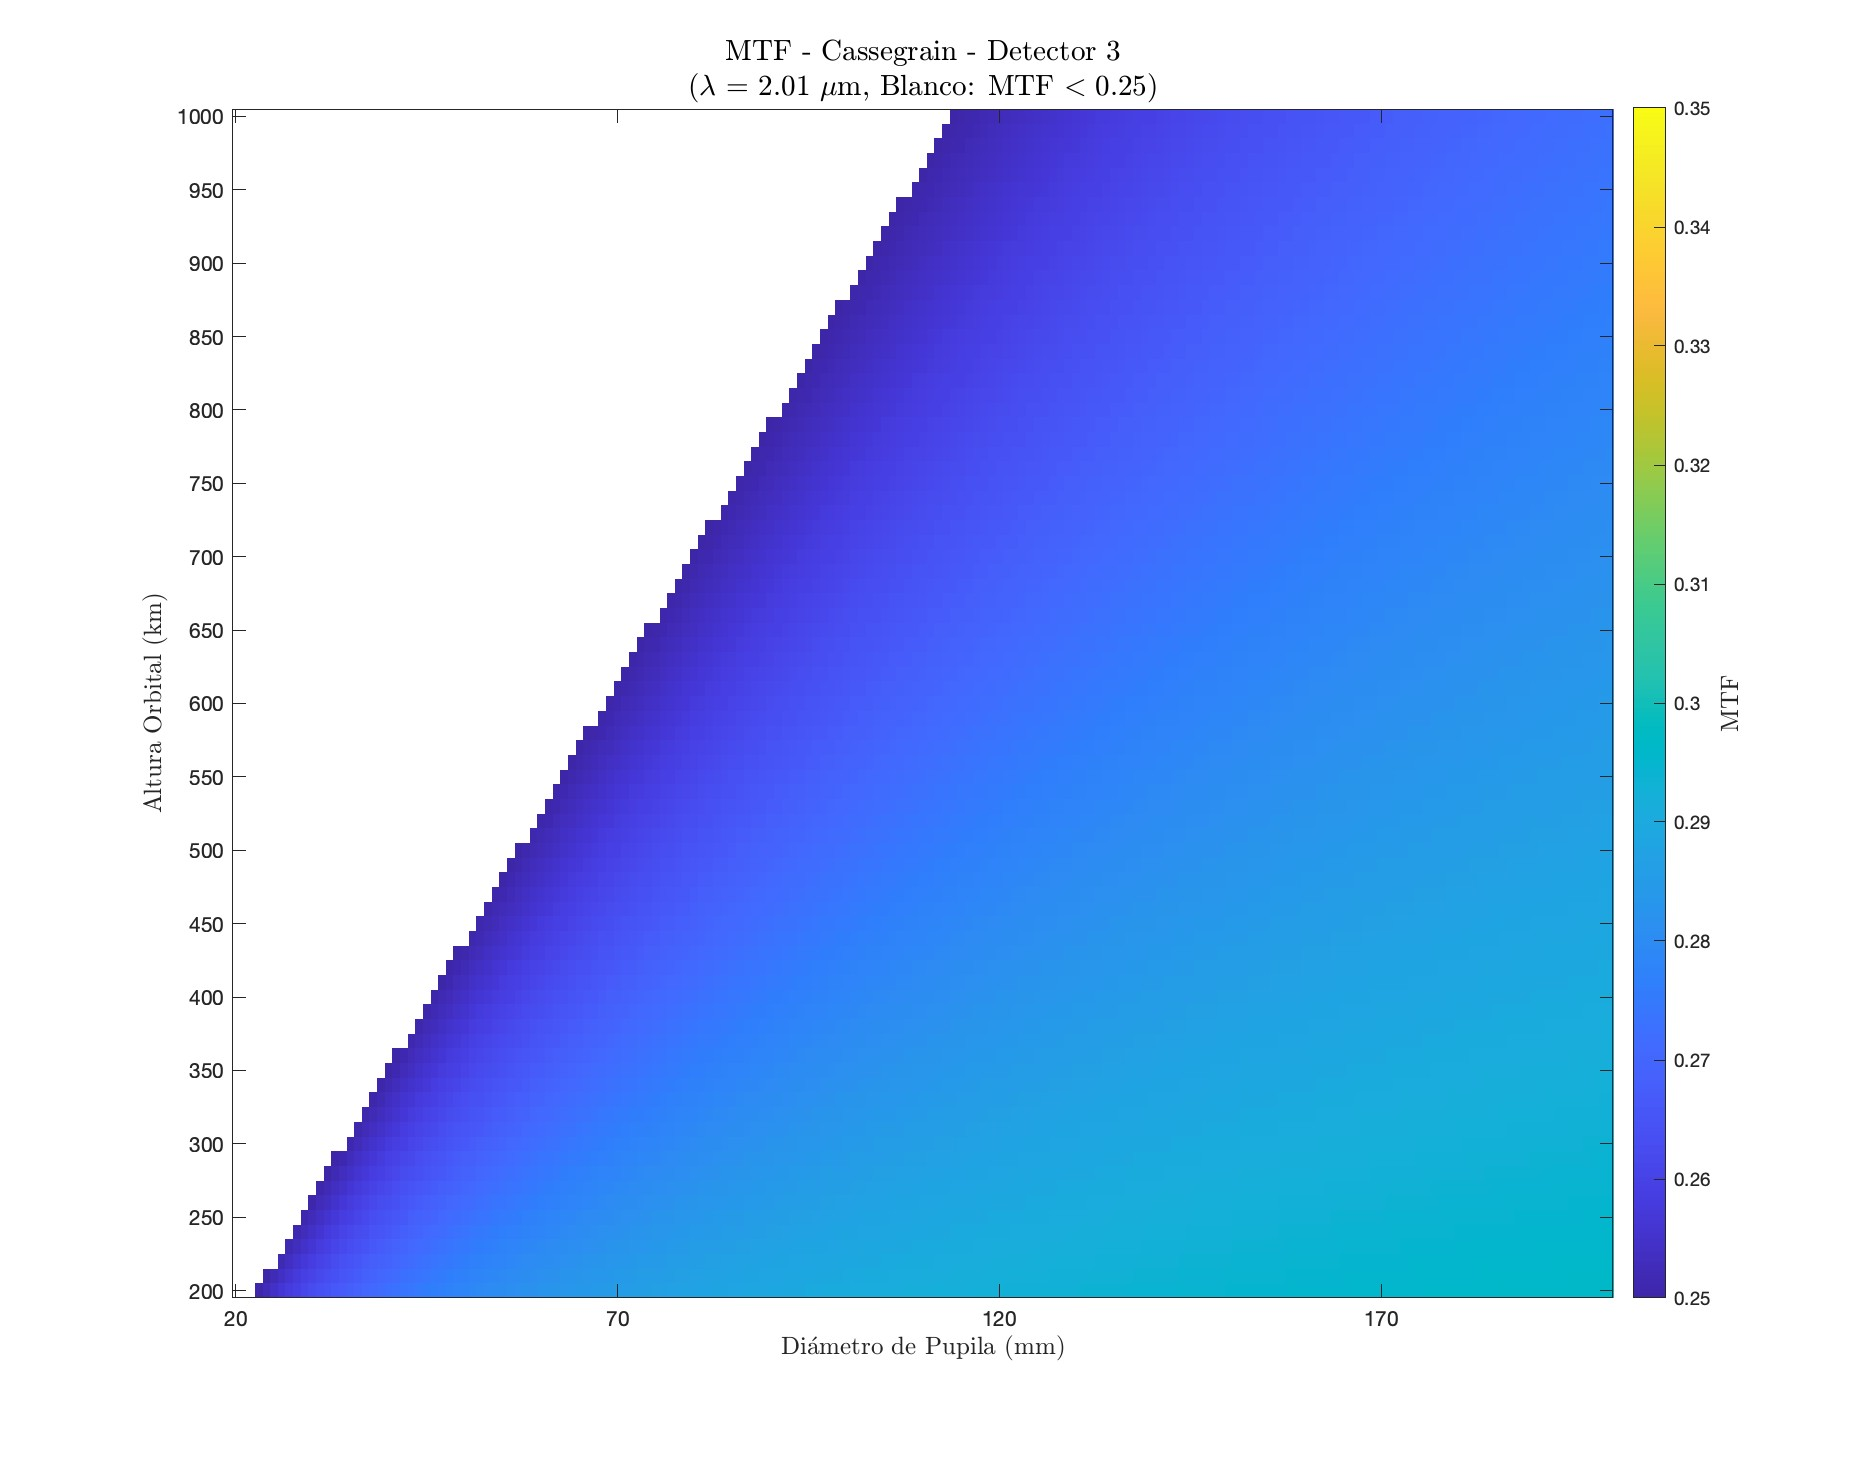
\includegraphics[width=0.48\linewidth]{4.Payload/MTF/MTF_Lambda2_Detector3_Telescopio3_heatmap.jpg} &
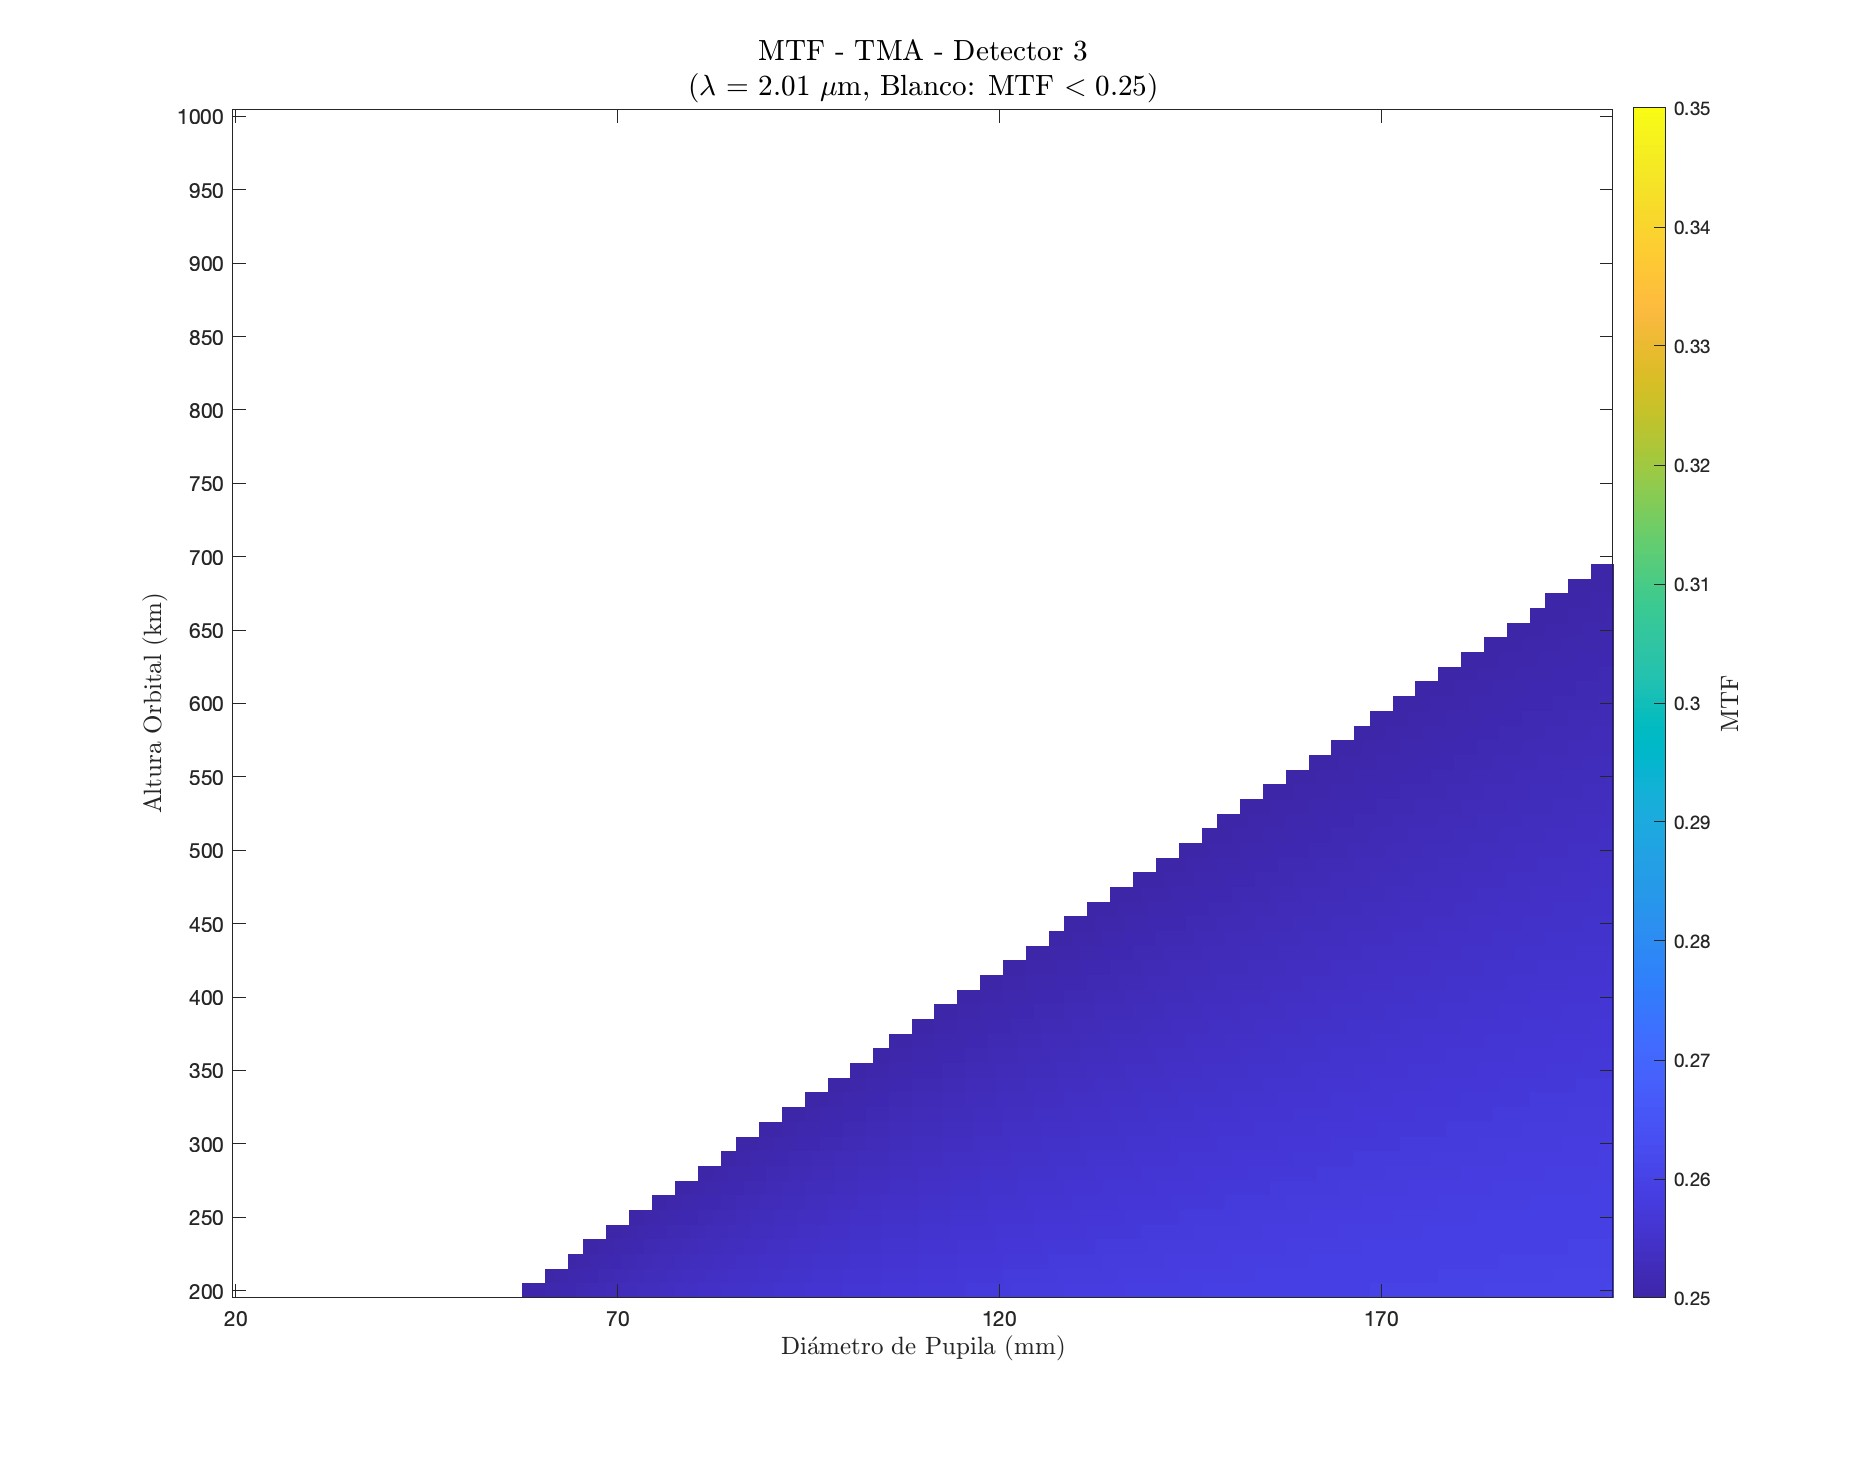
\includegraphics[width=0.48\linewidth]{4.Payload/MTF/MTF_Lambda2_Detector3_Telescopio4_heatmap.jpg} \\
\end{tabular}
\caption{Mapas de calor resultantes del calculo de MTF: Banda 2,01 \textmu m; Detector 3}
\end{figure}
\end{landscape}




\subsubsection{SNR}
\addcontentsline{toc}{section}{SNR}

%========================================================================================
%                                     LAMBDA 3
%========================================================================================
%% DETECTOR 4
\begin{landscape}
\begin{figure}[p]
\centering
\setlength{\tabcolsep}{2pt}
\renewcommand{\arraystretch}{0}

\paragraph{Banda 0,76 \textmu m}
\begin{tabular}{cc}
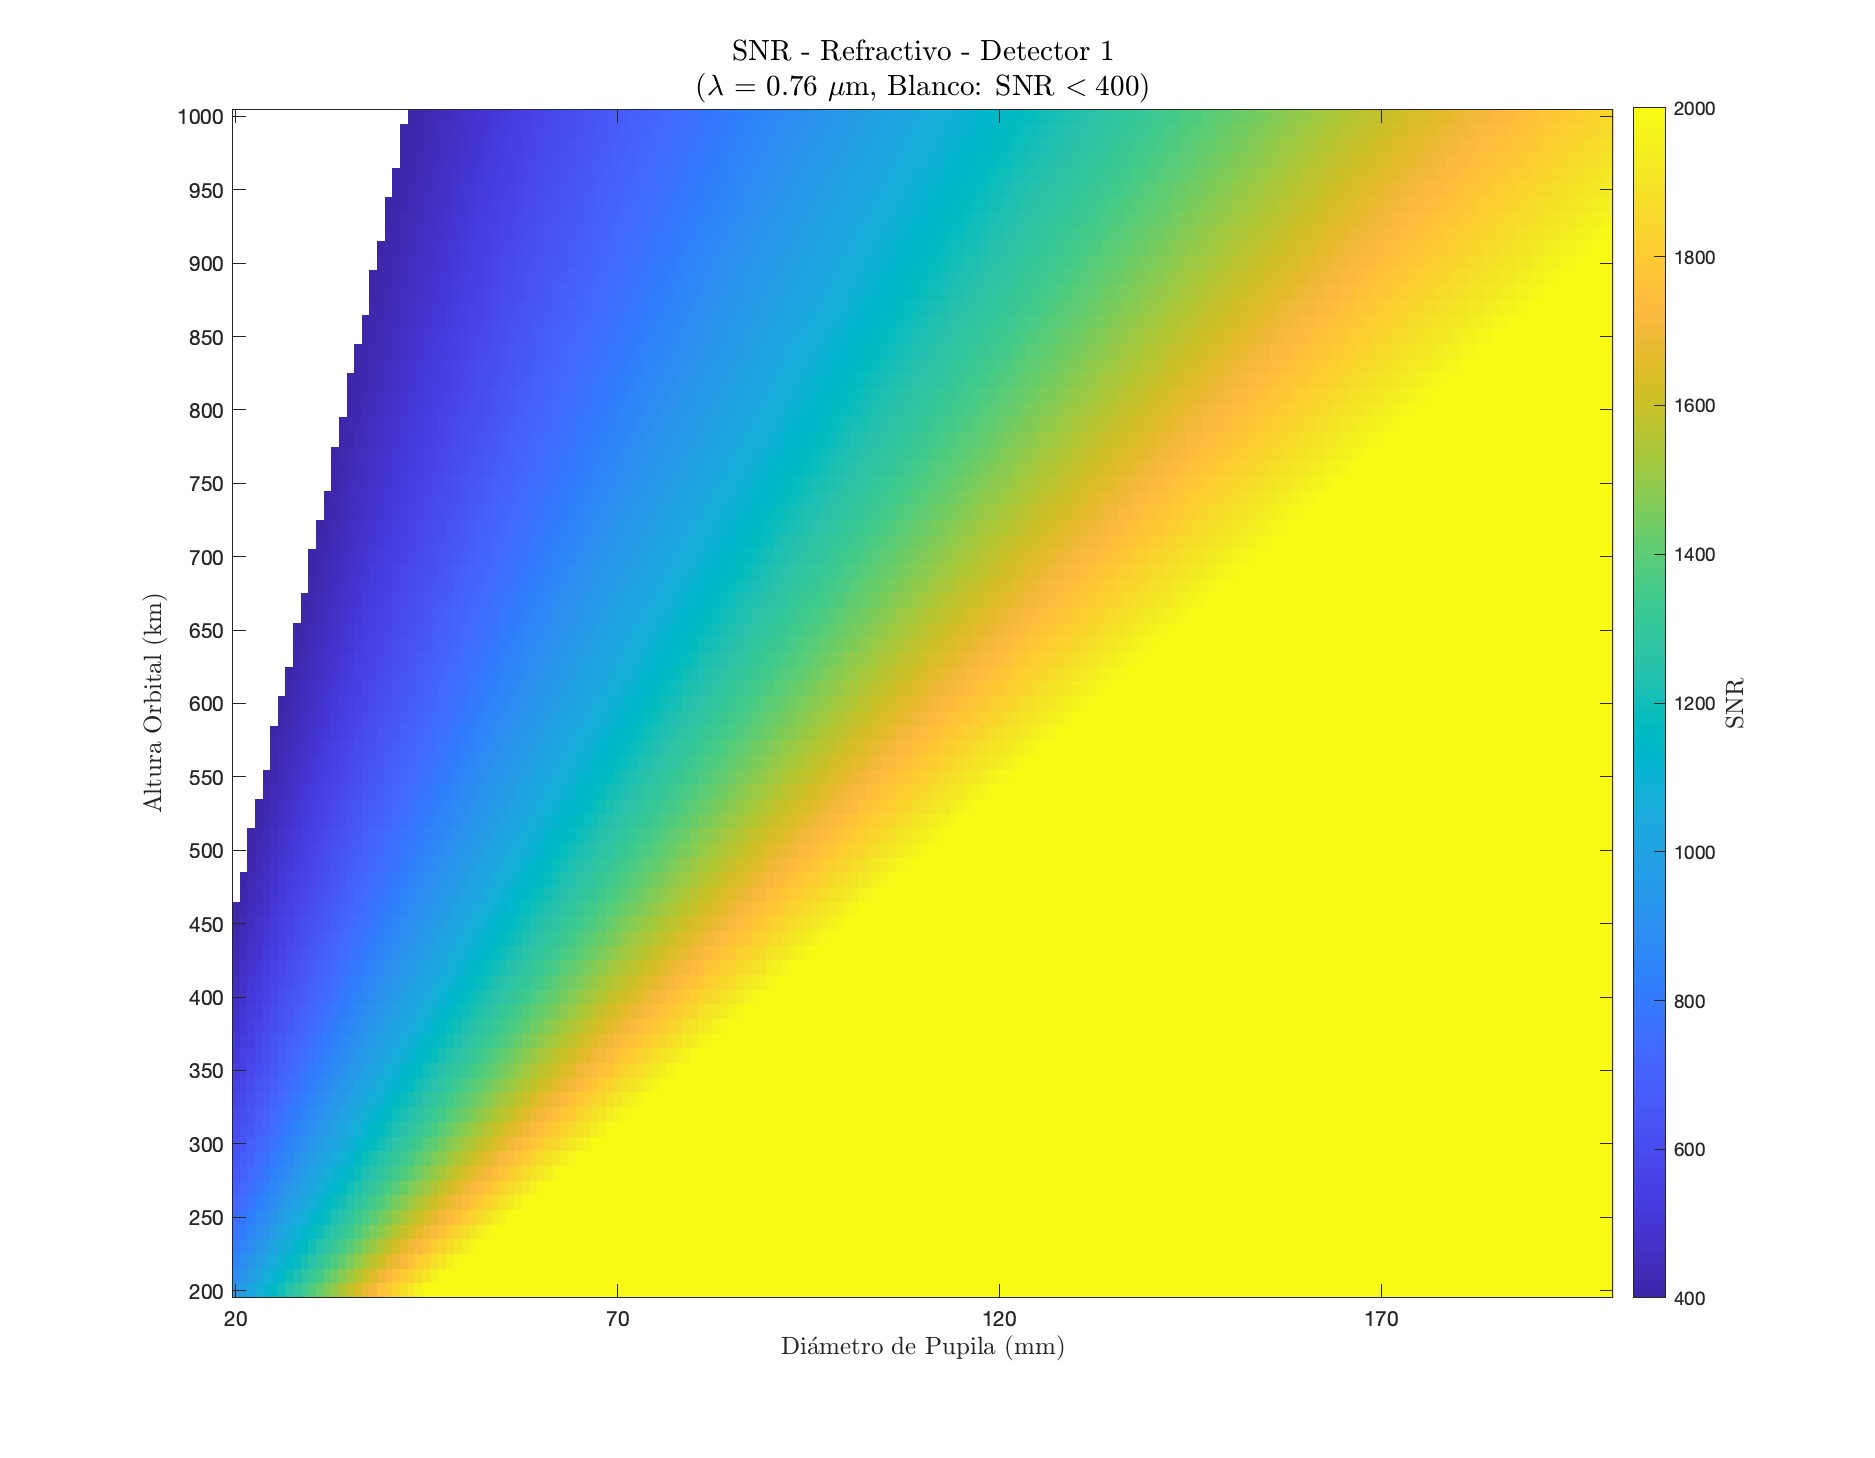
\includegraphics[width=0.48\linewidth]{4.Payload/SNR/SNR_Lambda3_Detector4_Telescopio1_heatmap.jpg} &
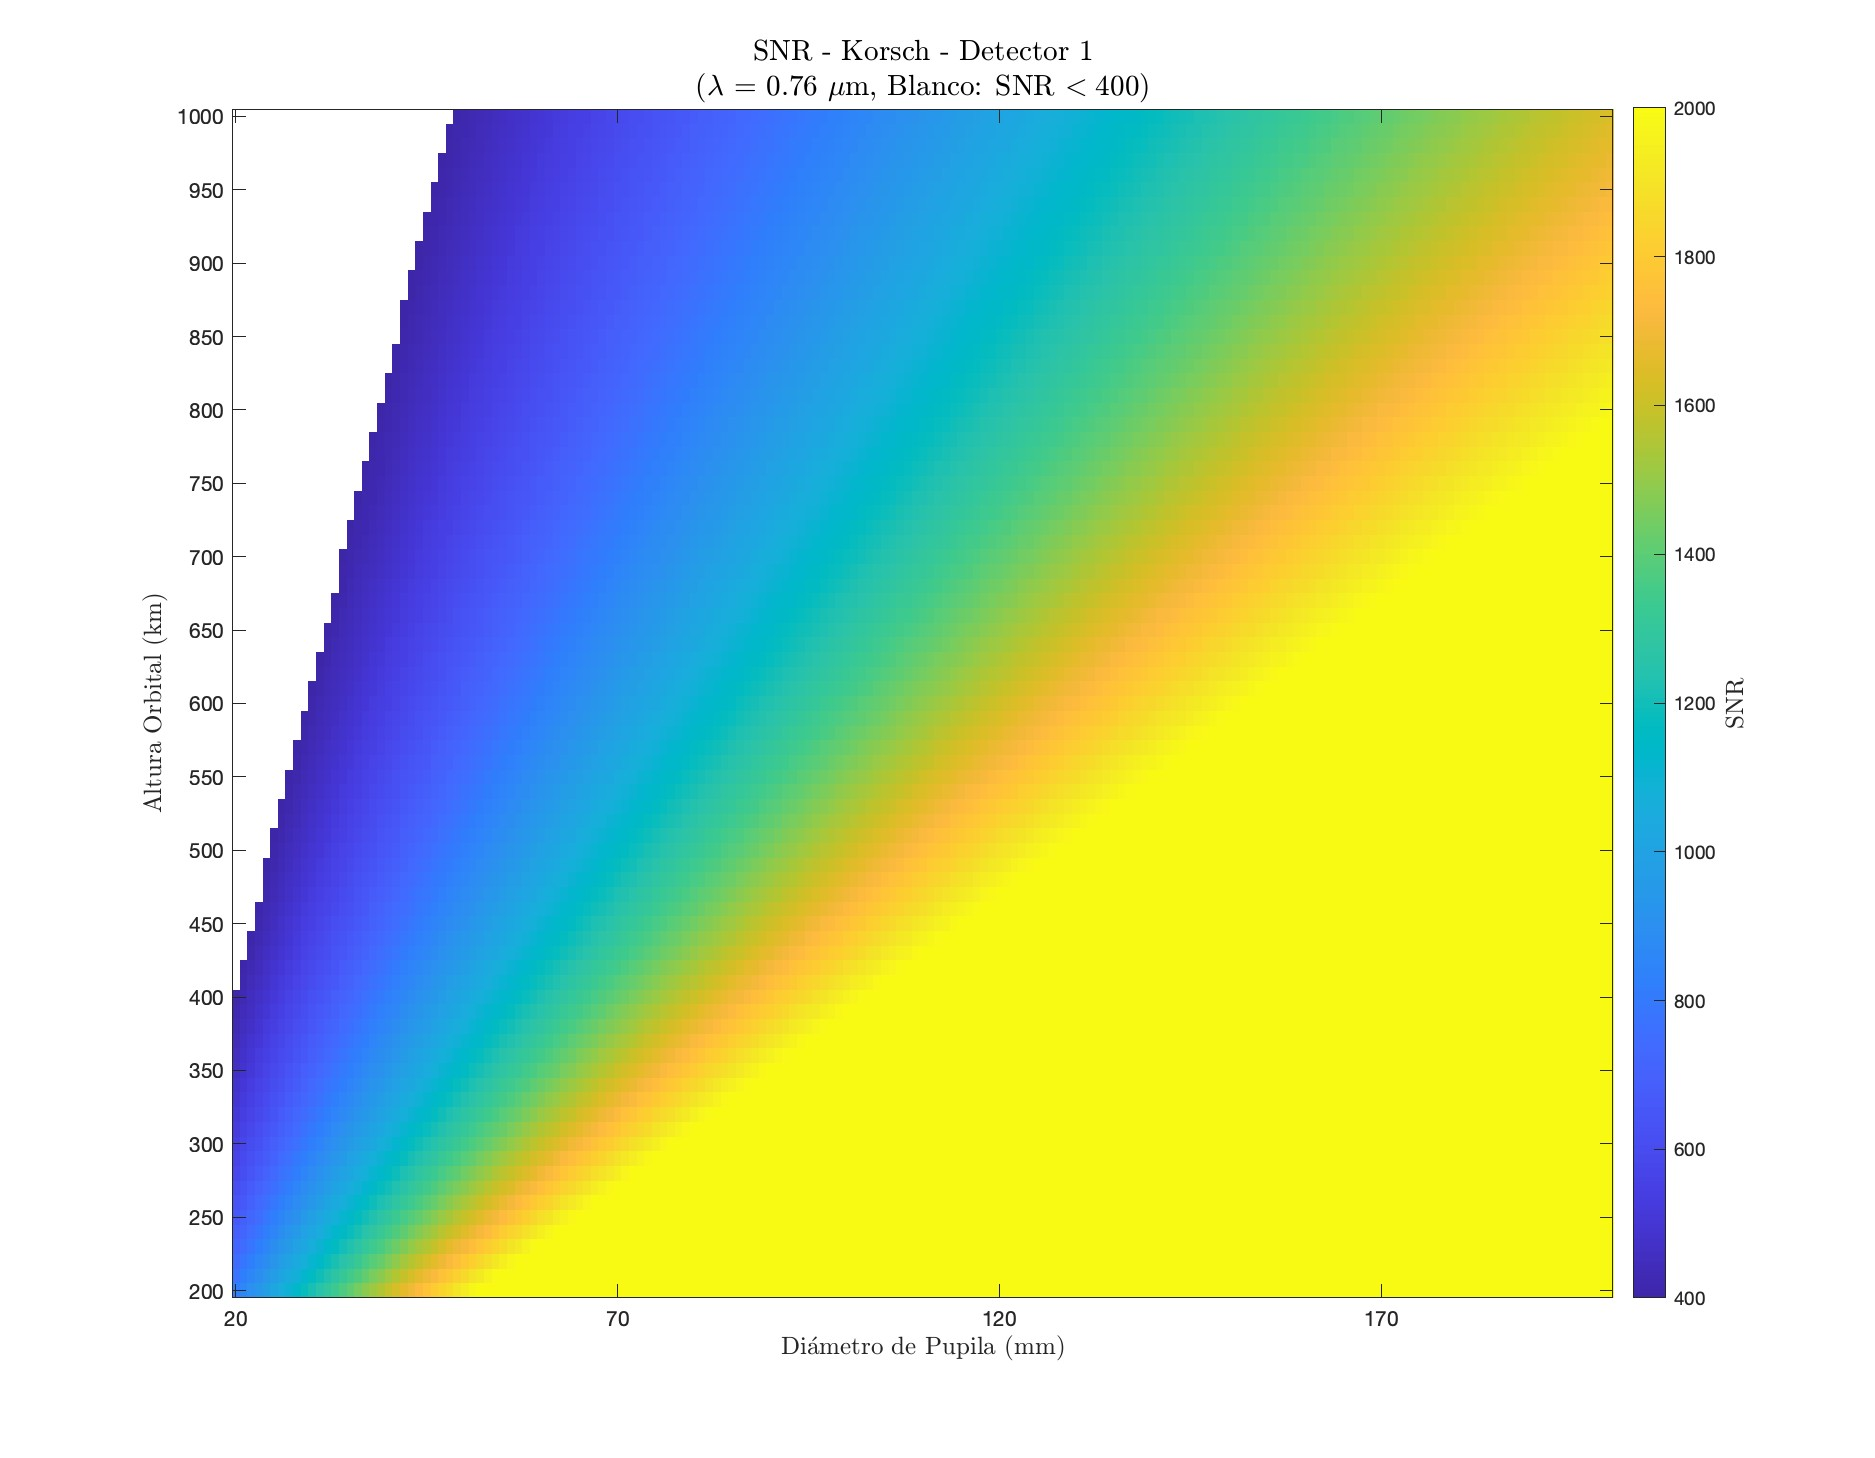
\includegraphics[width=0.48\linewidth]{4.Payload/SNR/SNR_Lambda3_Detector4_Telescopio2_heatmap.jpg} \\
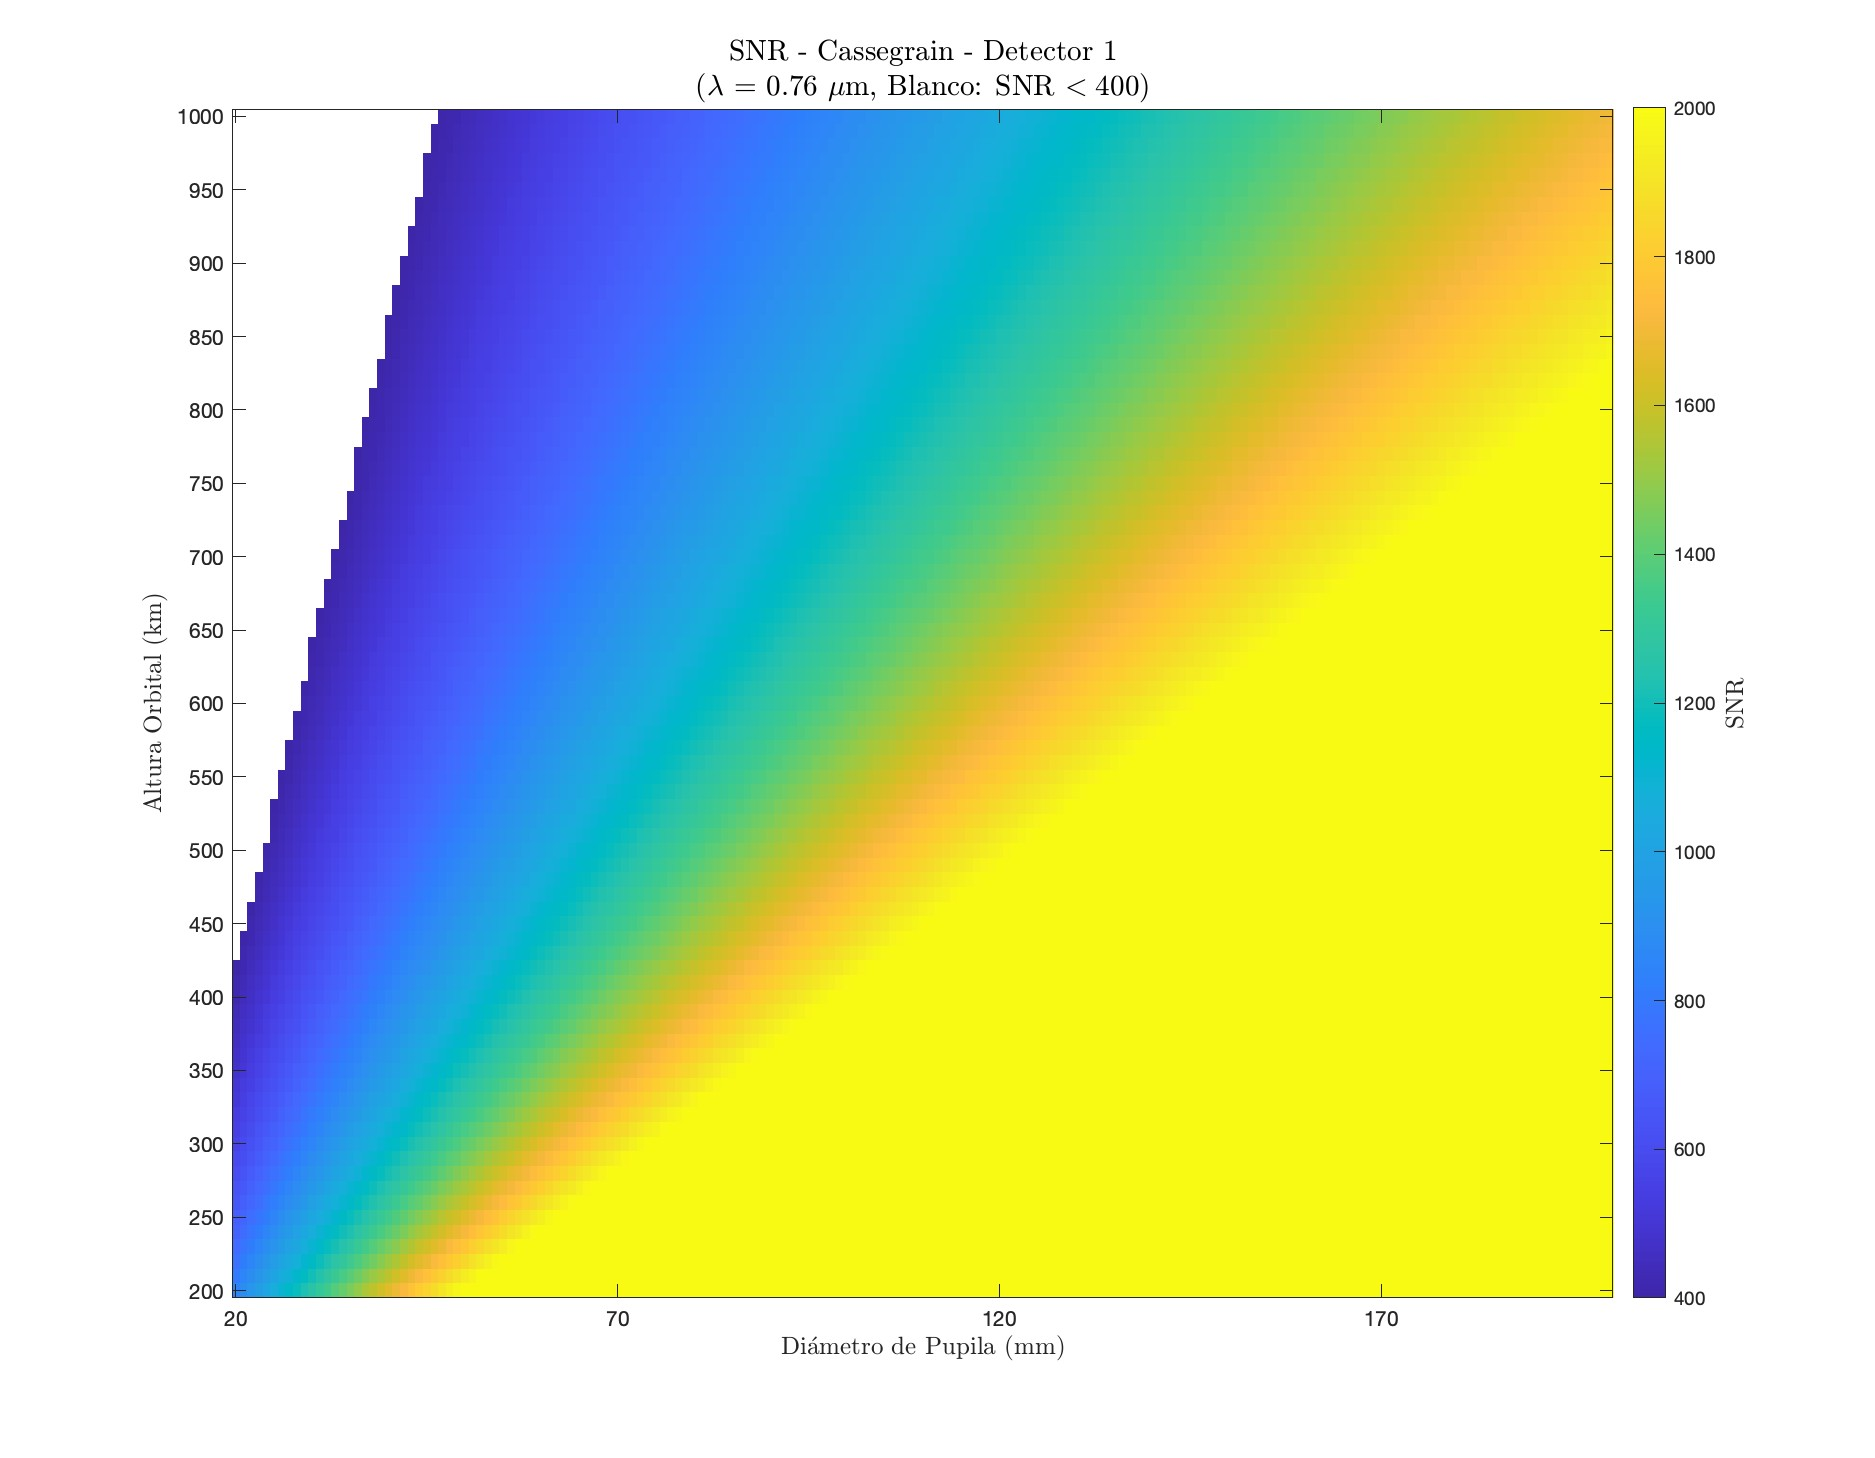
\includegraphics[width=0.48\linewidth]{4.Payload/SNR/SNR_Lambda3_Detector4_Telescopio3_heatmap.jpg} &
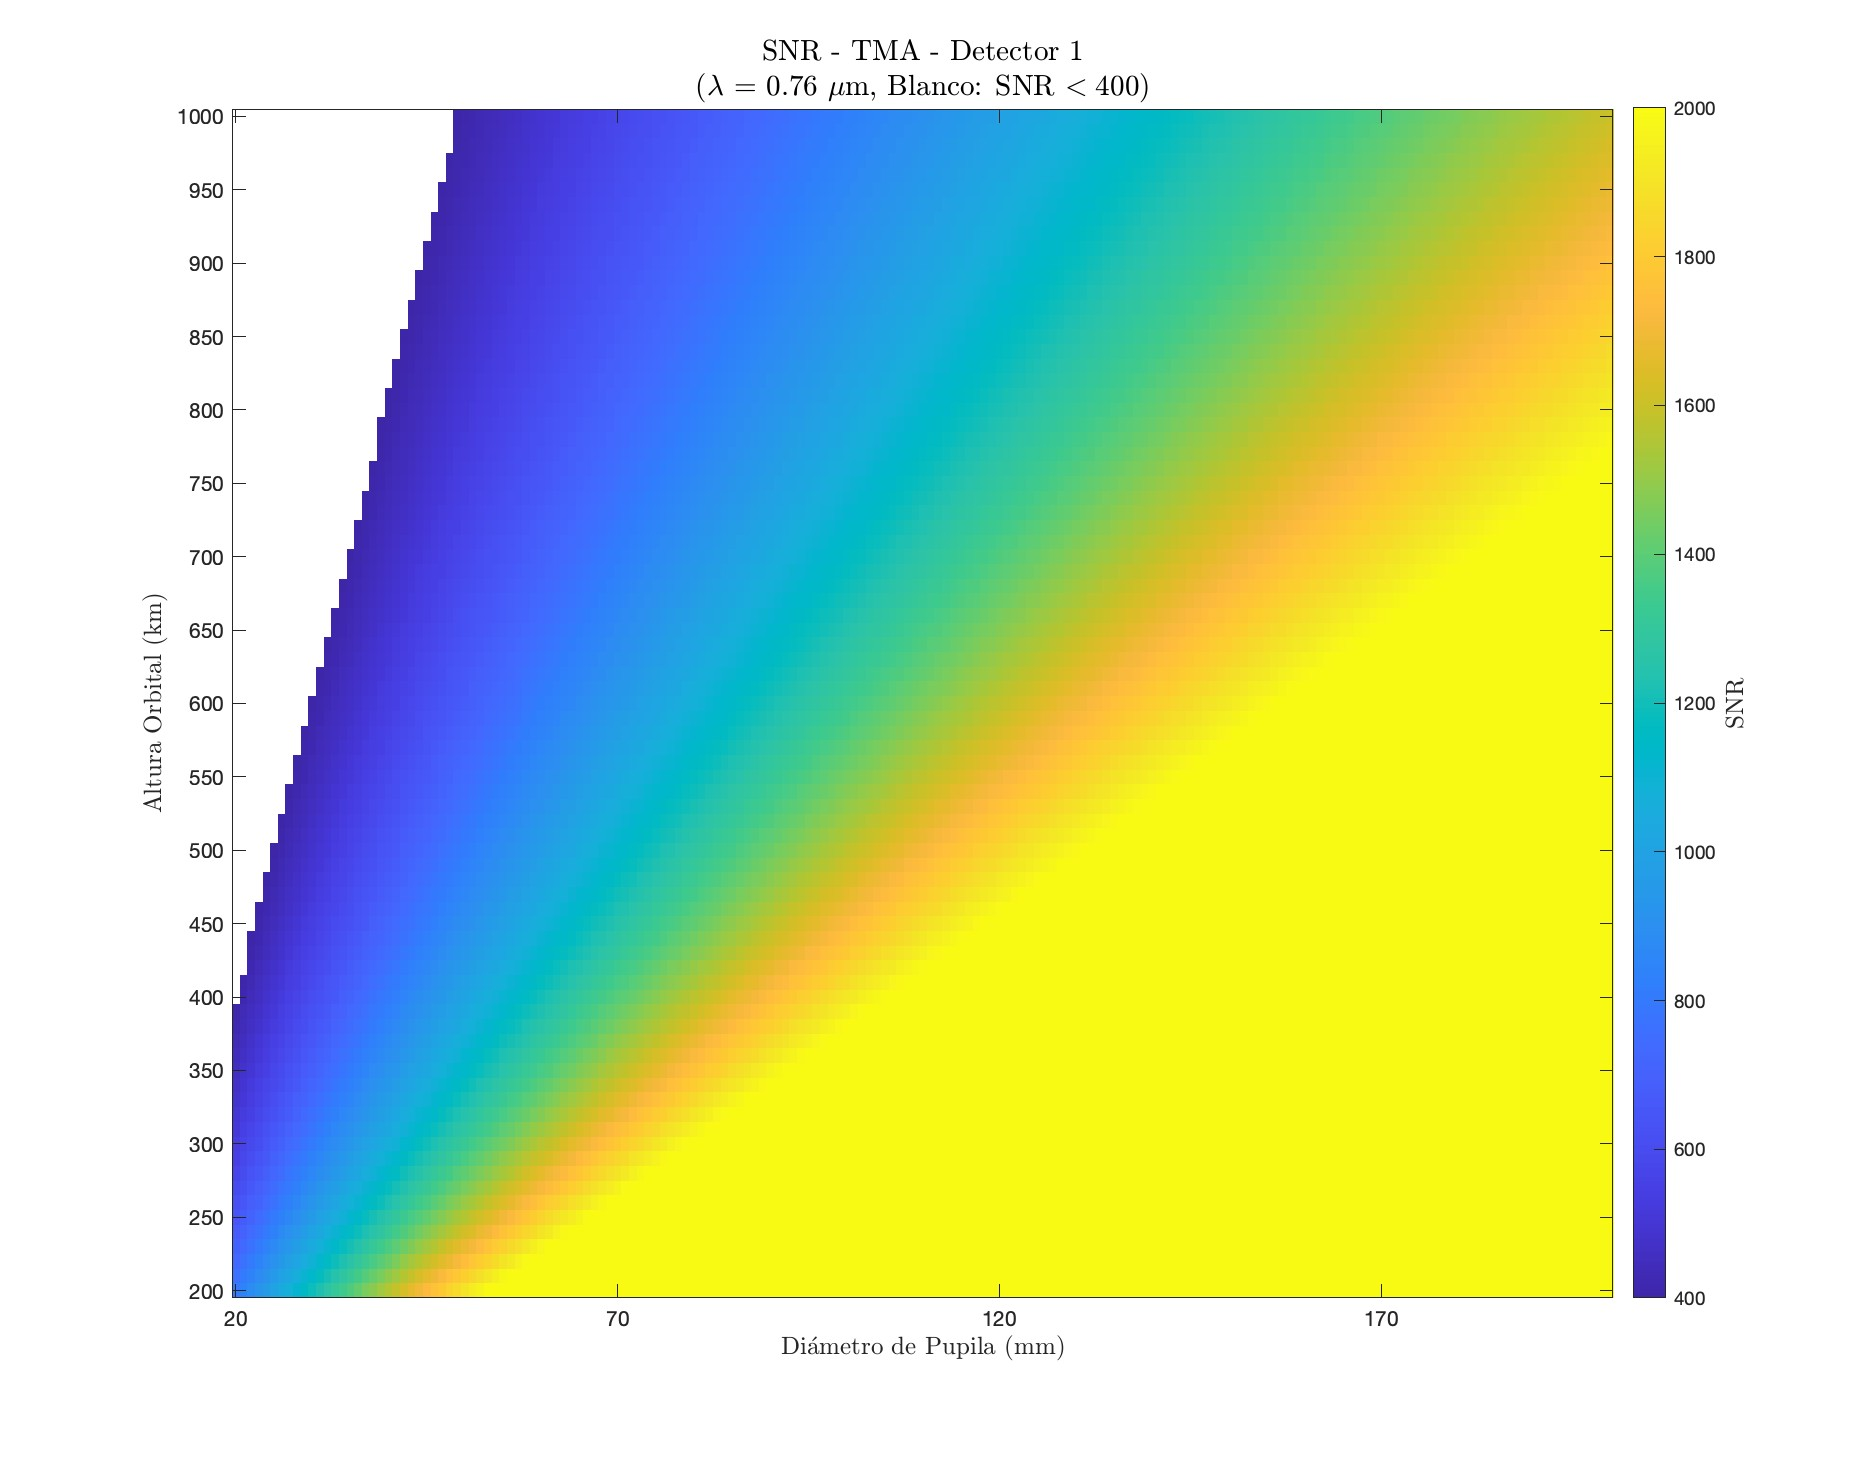
\includegraphics[width=0.48\linewidth]{4.Payload/SNR/SNR_Lambda3_Detector4_Telescopio4_heatmap.jpg} \\
\end{tabular}
% Nota: Reemplazar "0,76" con el valor de longitud de onda para Lambda 3.
\caption{Mapas de calor resultantes del calculo de SNR: Banda 0,76 \textmu m; Detector 4}
\end{figure}
\end{landscape}


%% DETECTOR 5
\begin{landscape}
\begin{figure}[p]
\centering
\setlength{\tabcolsep}{2pt}
\renewcommand{\arraystretch}{0}

\paragraph{Banda 0,76 \textmu m}
\begin{tabular}{cc}
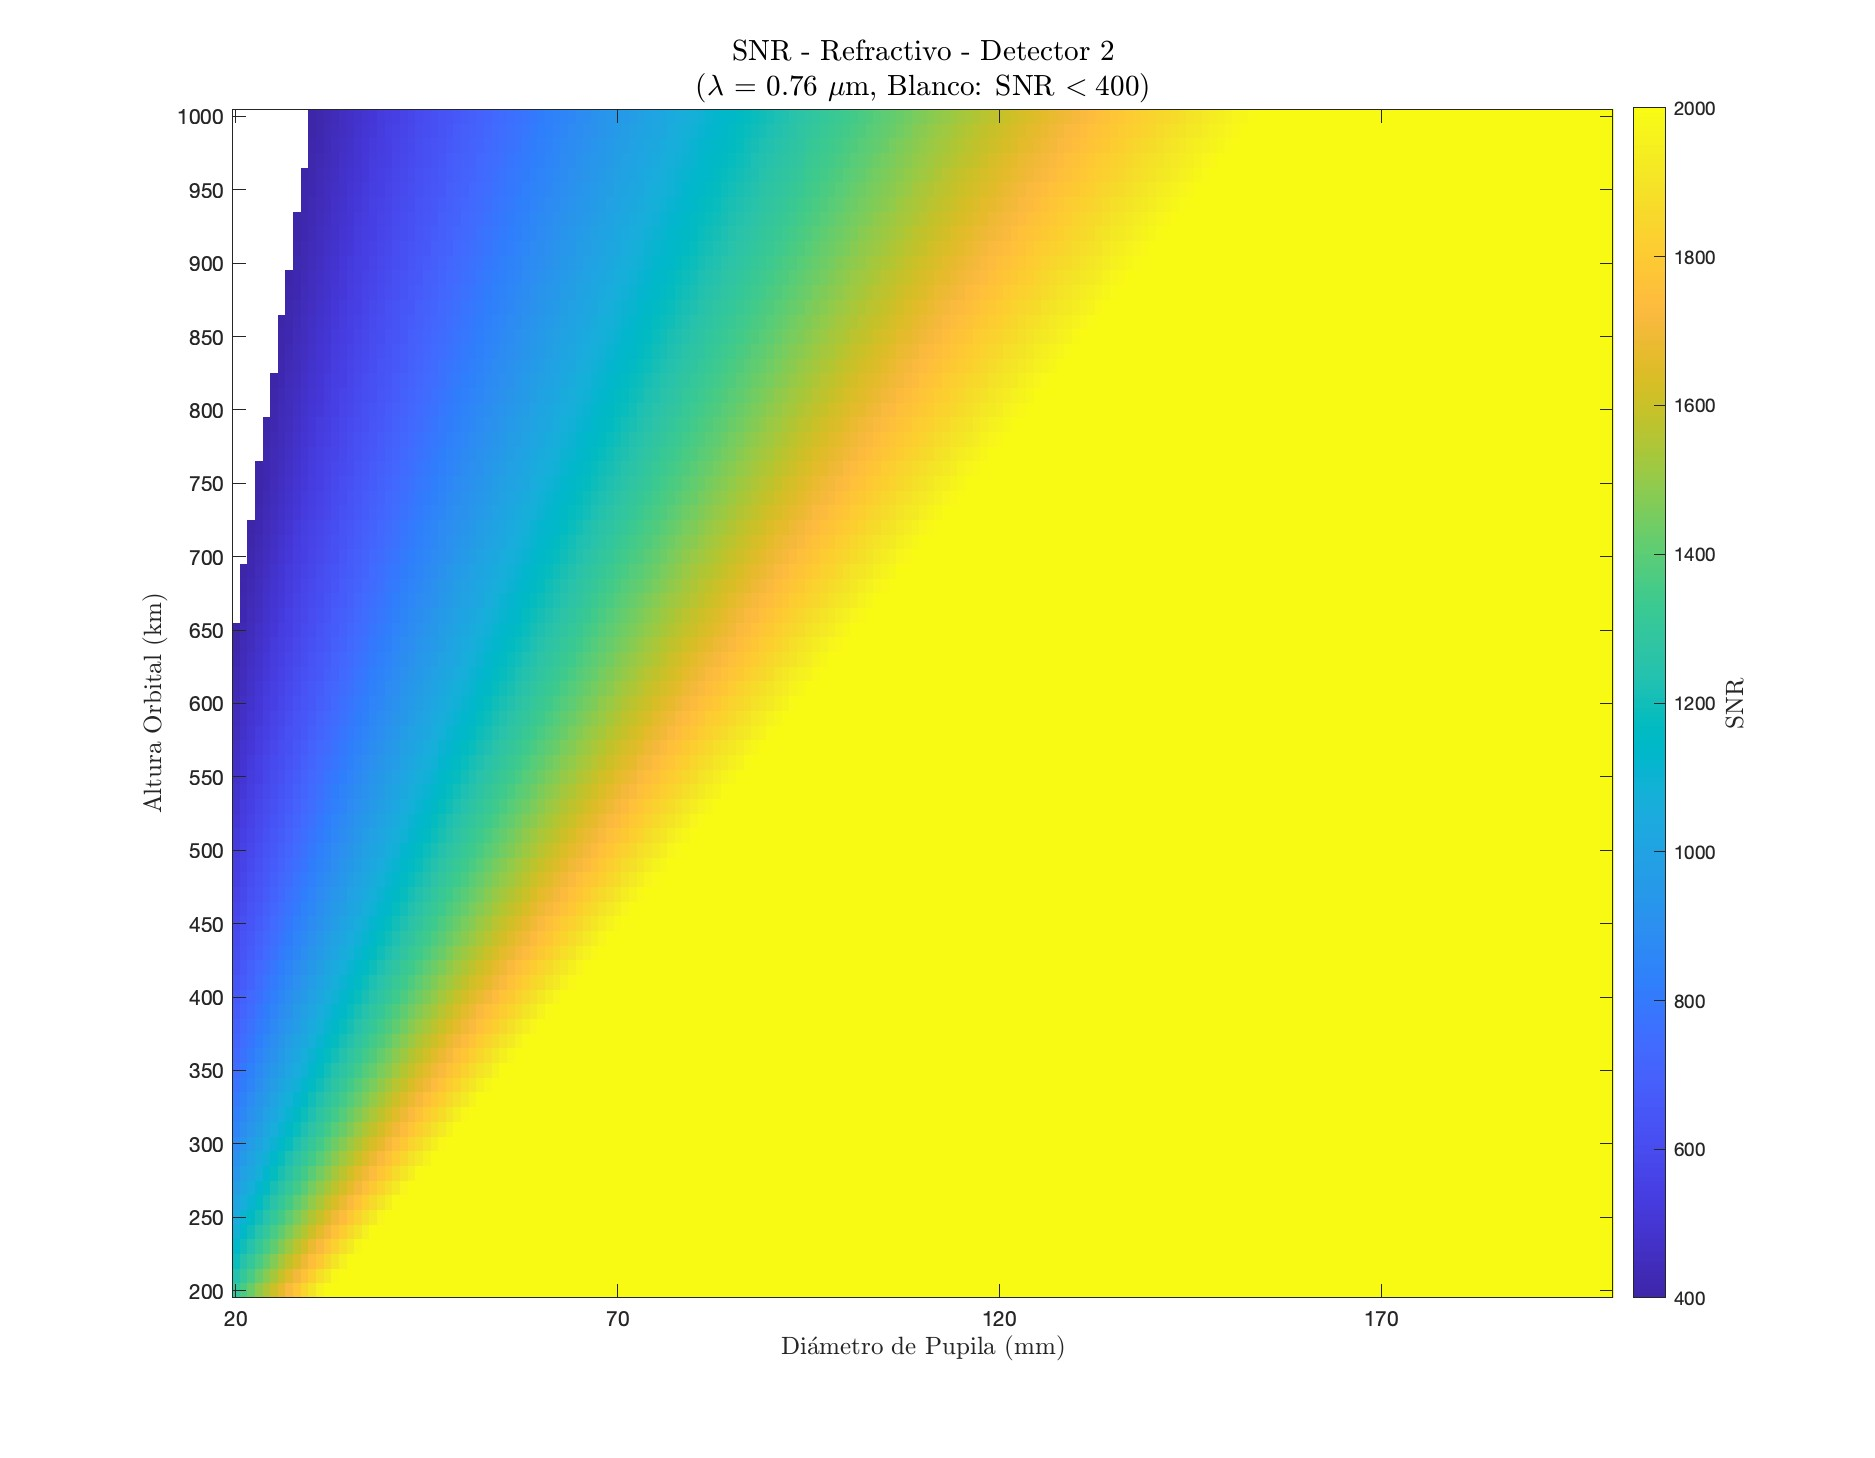
\includegraphics[width=0.48\linewidth]{4.Payload/SNR/SNR_Lambda3_Detector5_Telescopio1_heatmap.jpg} &
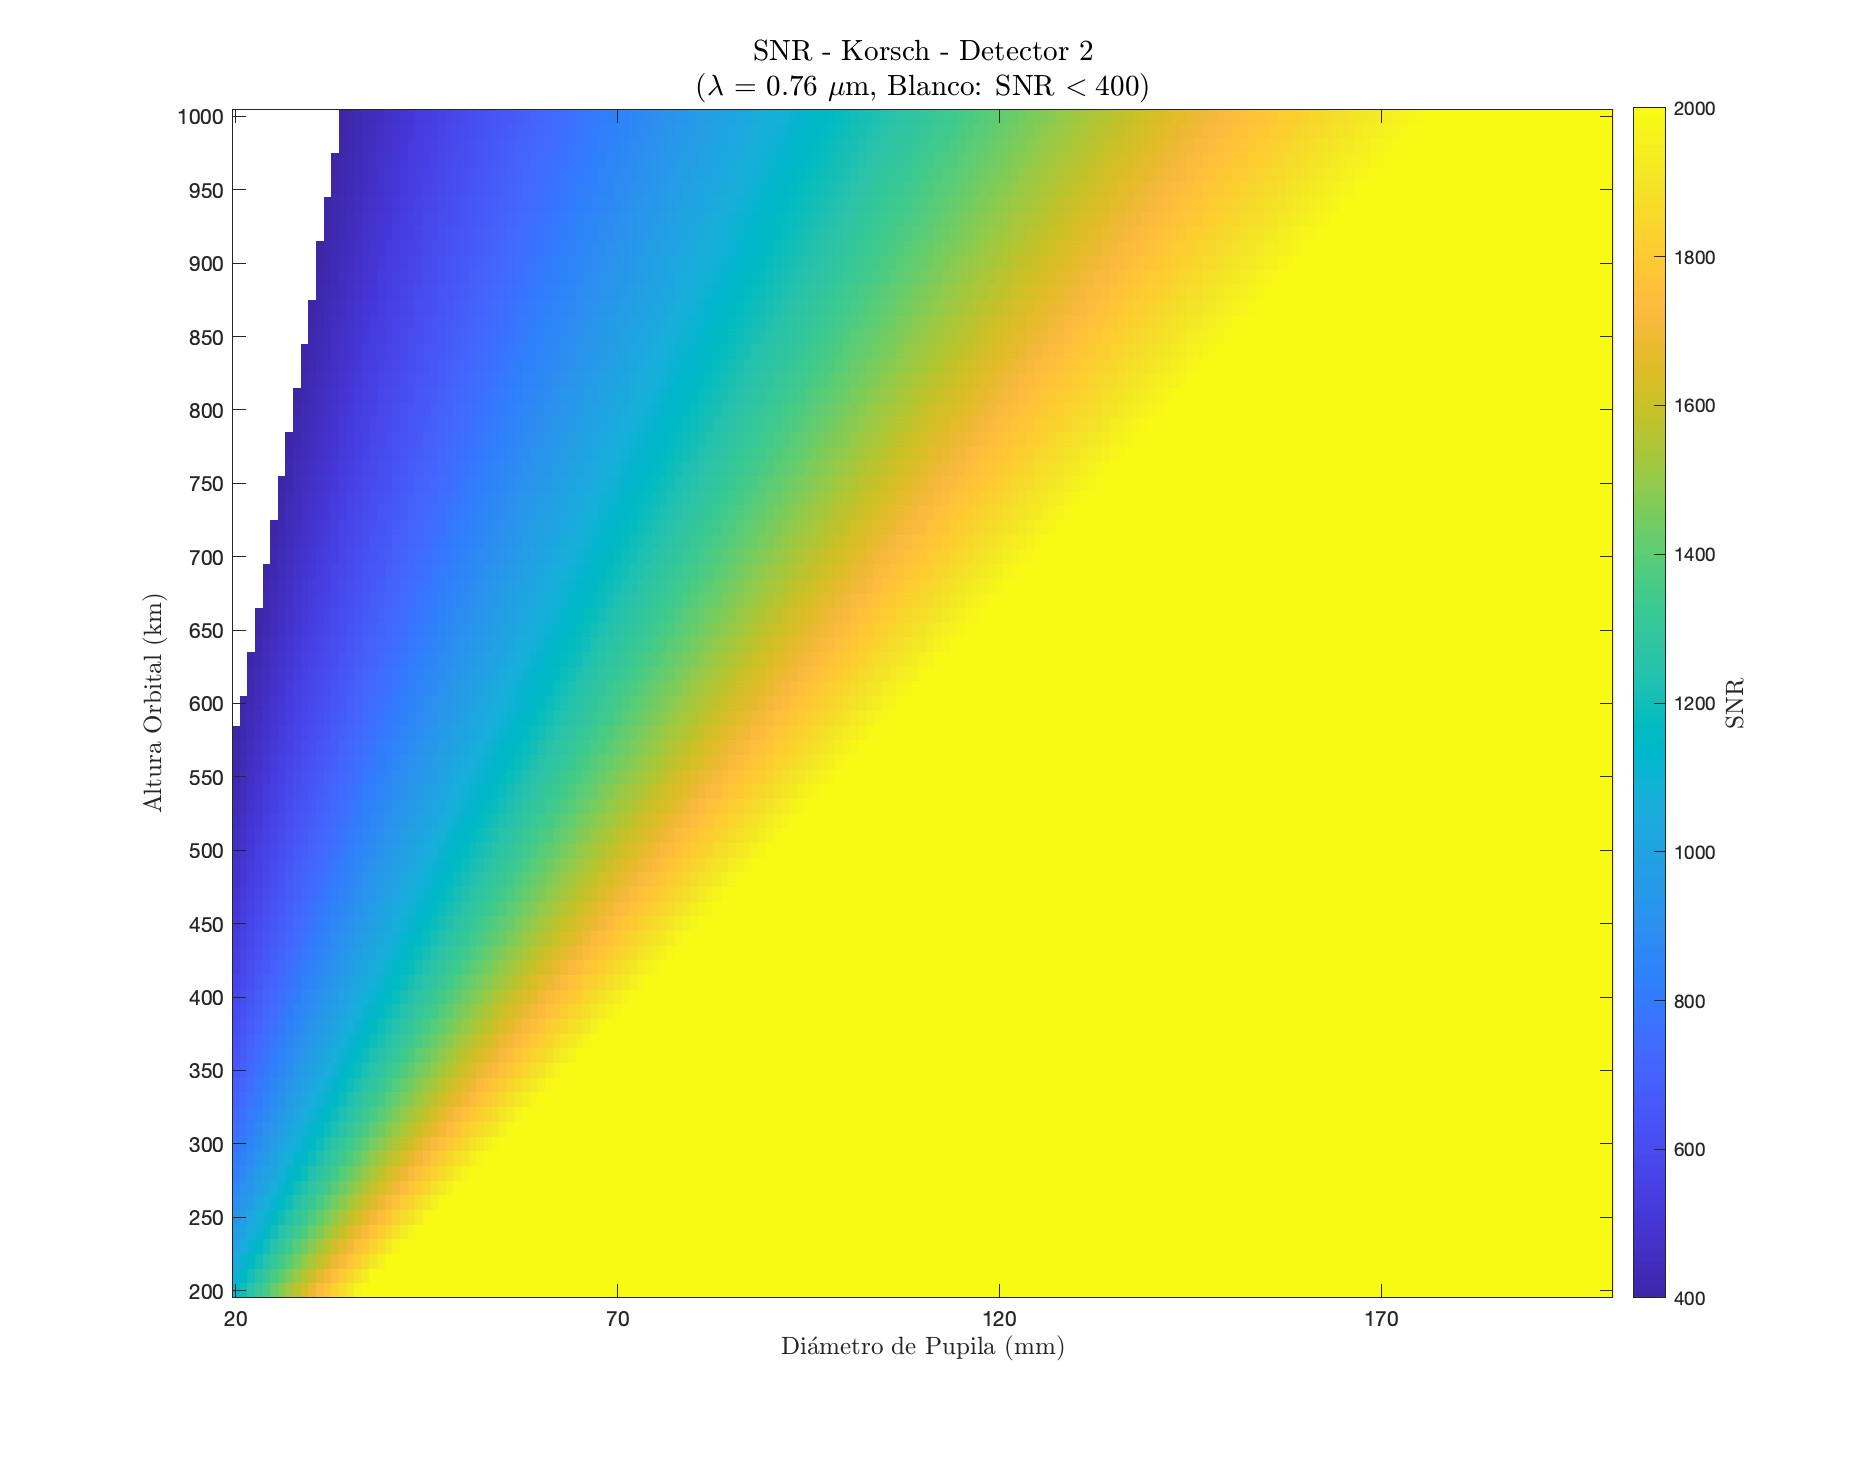
\includegraphics[width=0.48\linewidth]{4.Payload/SNR/SNR_Lambda3_Detector5_Telescopio2_heatmap.jpg} \\
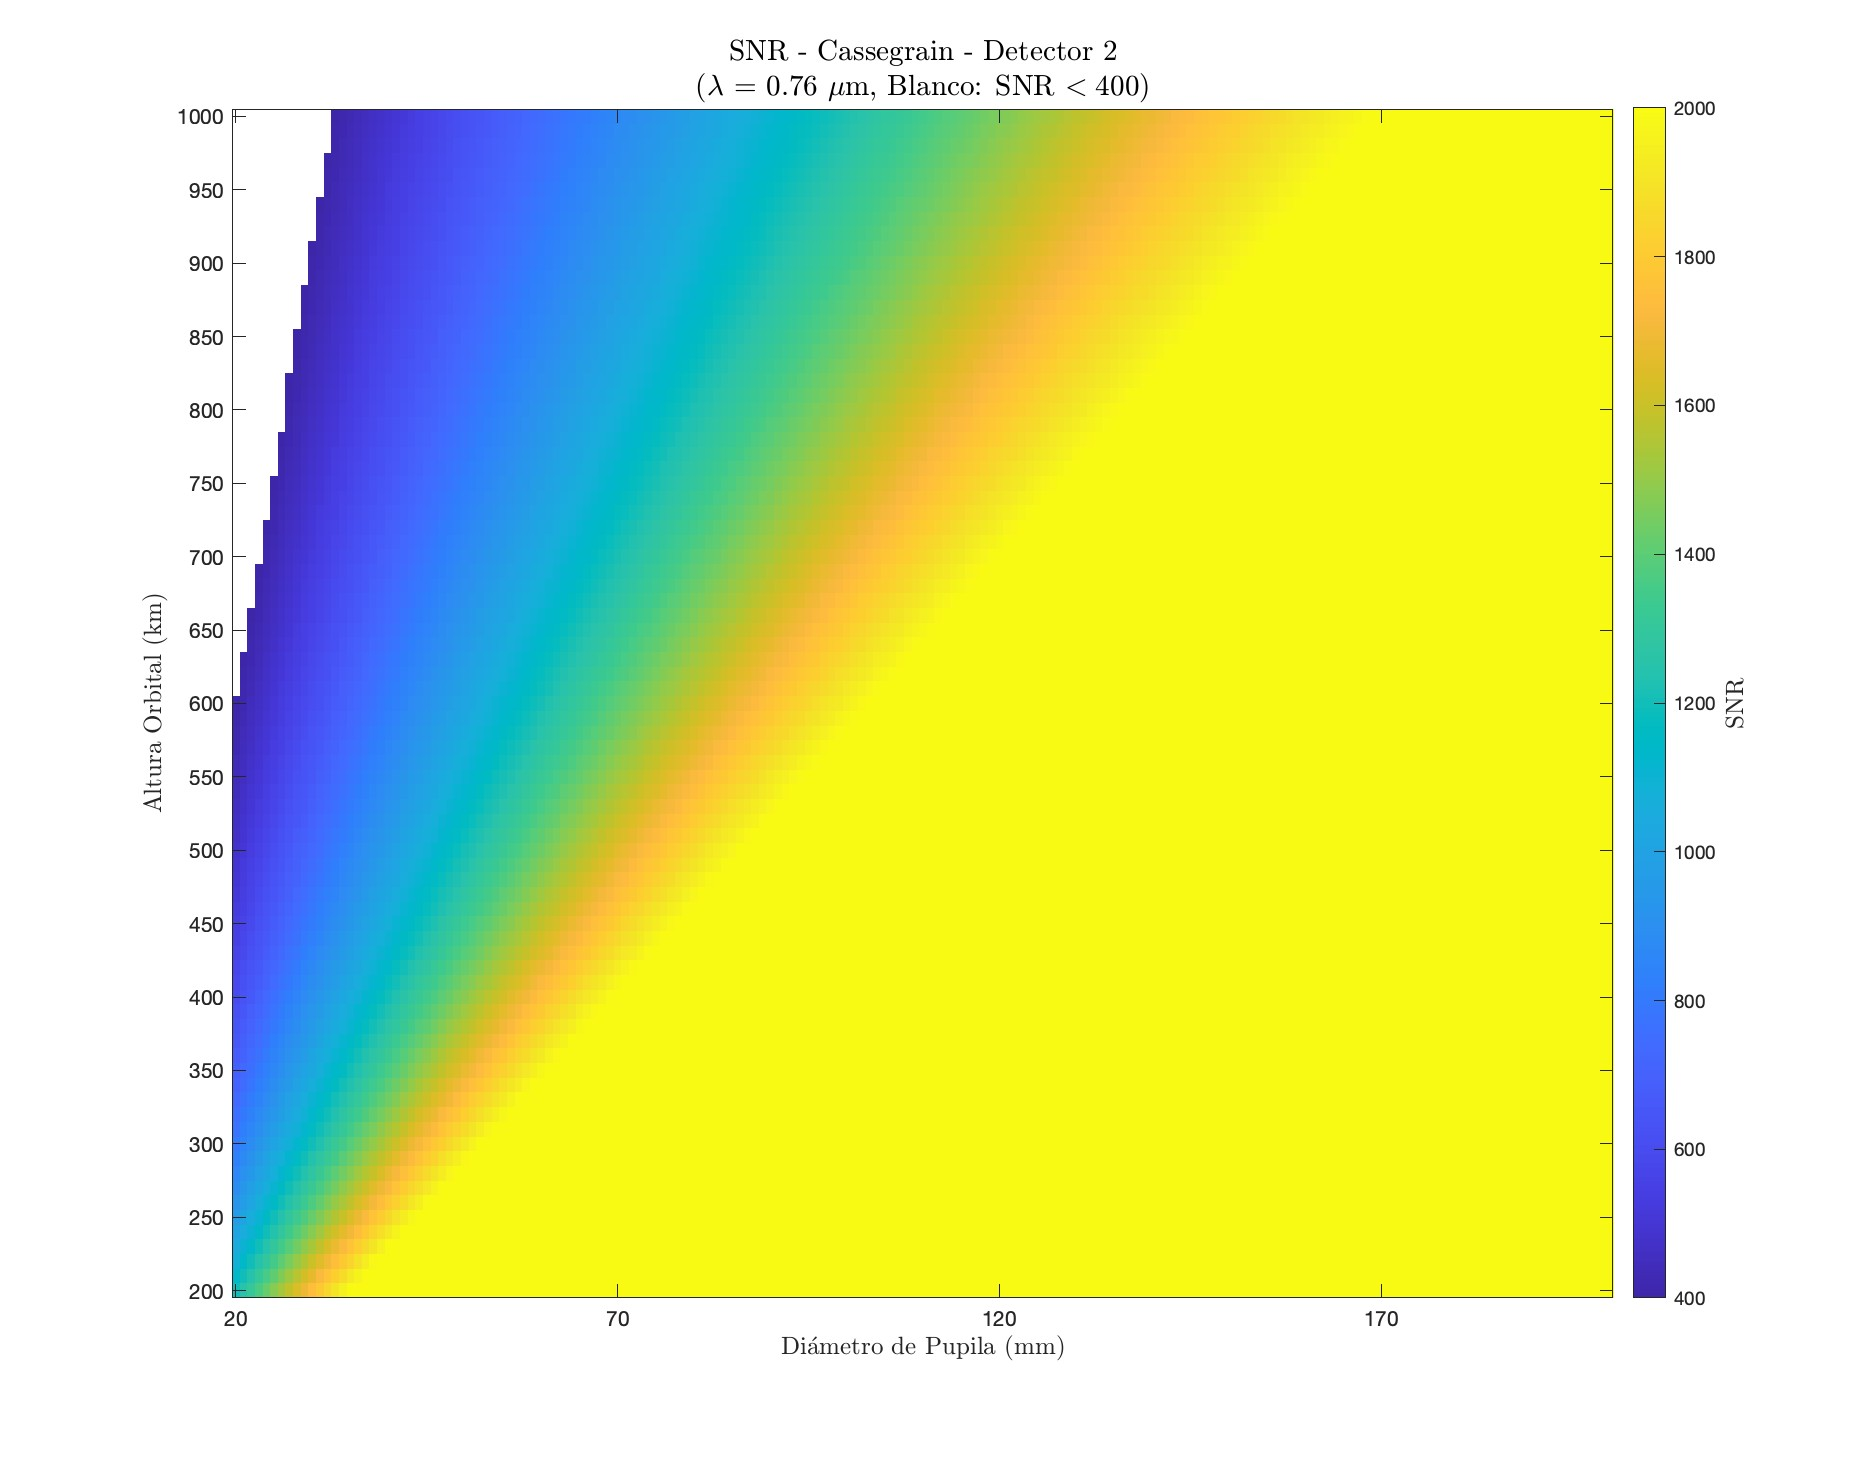
\includegraphics[width=0.48\linewidth]{4.Payload/SNR/SNR_Lambda3_Detector5_Telescopio3_heatmap.jpg} &
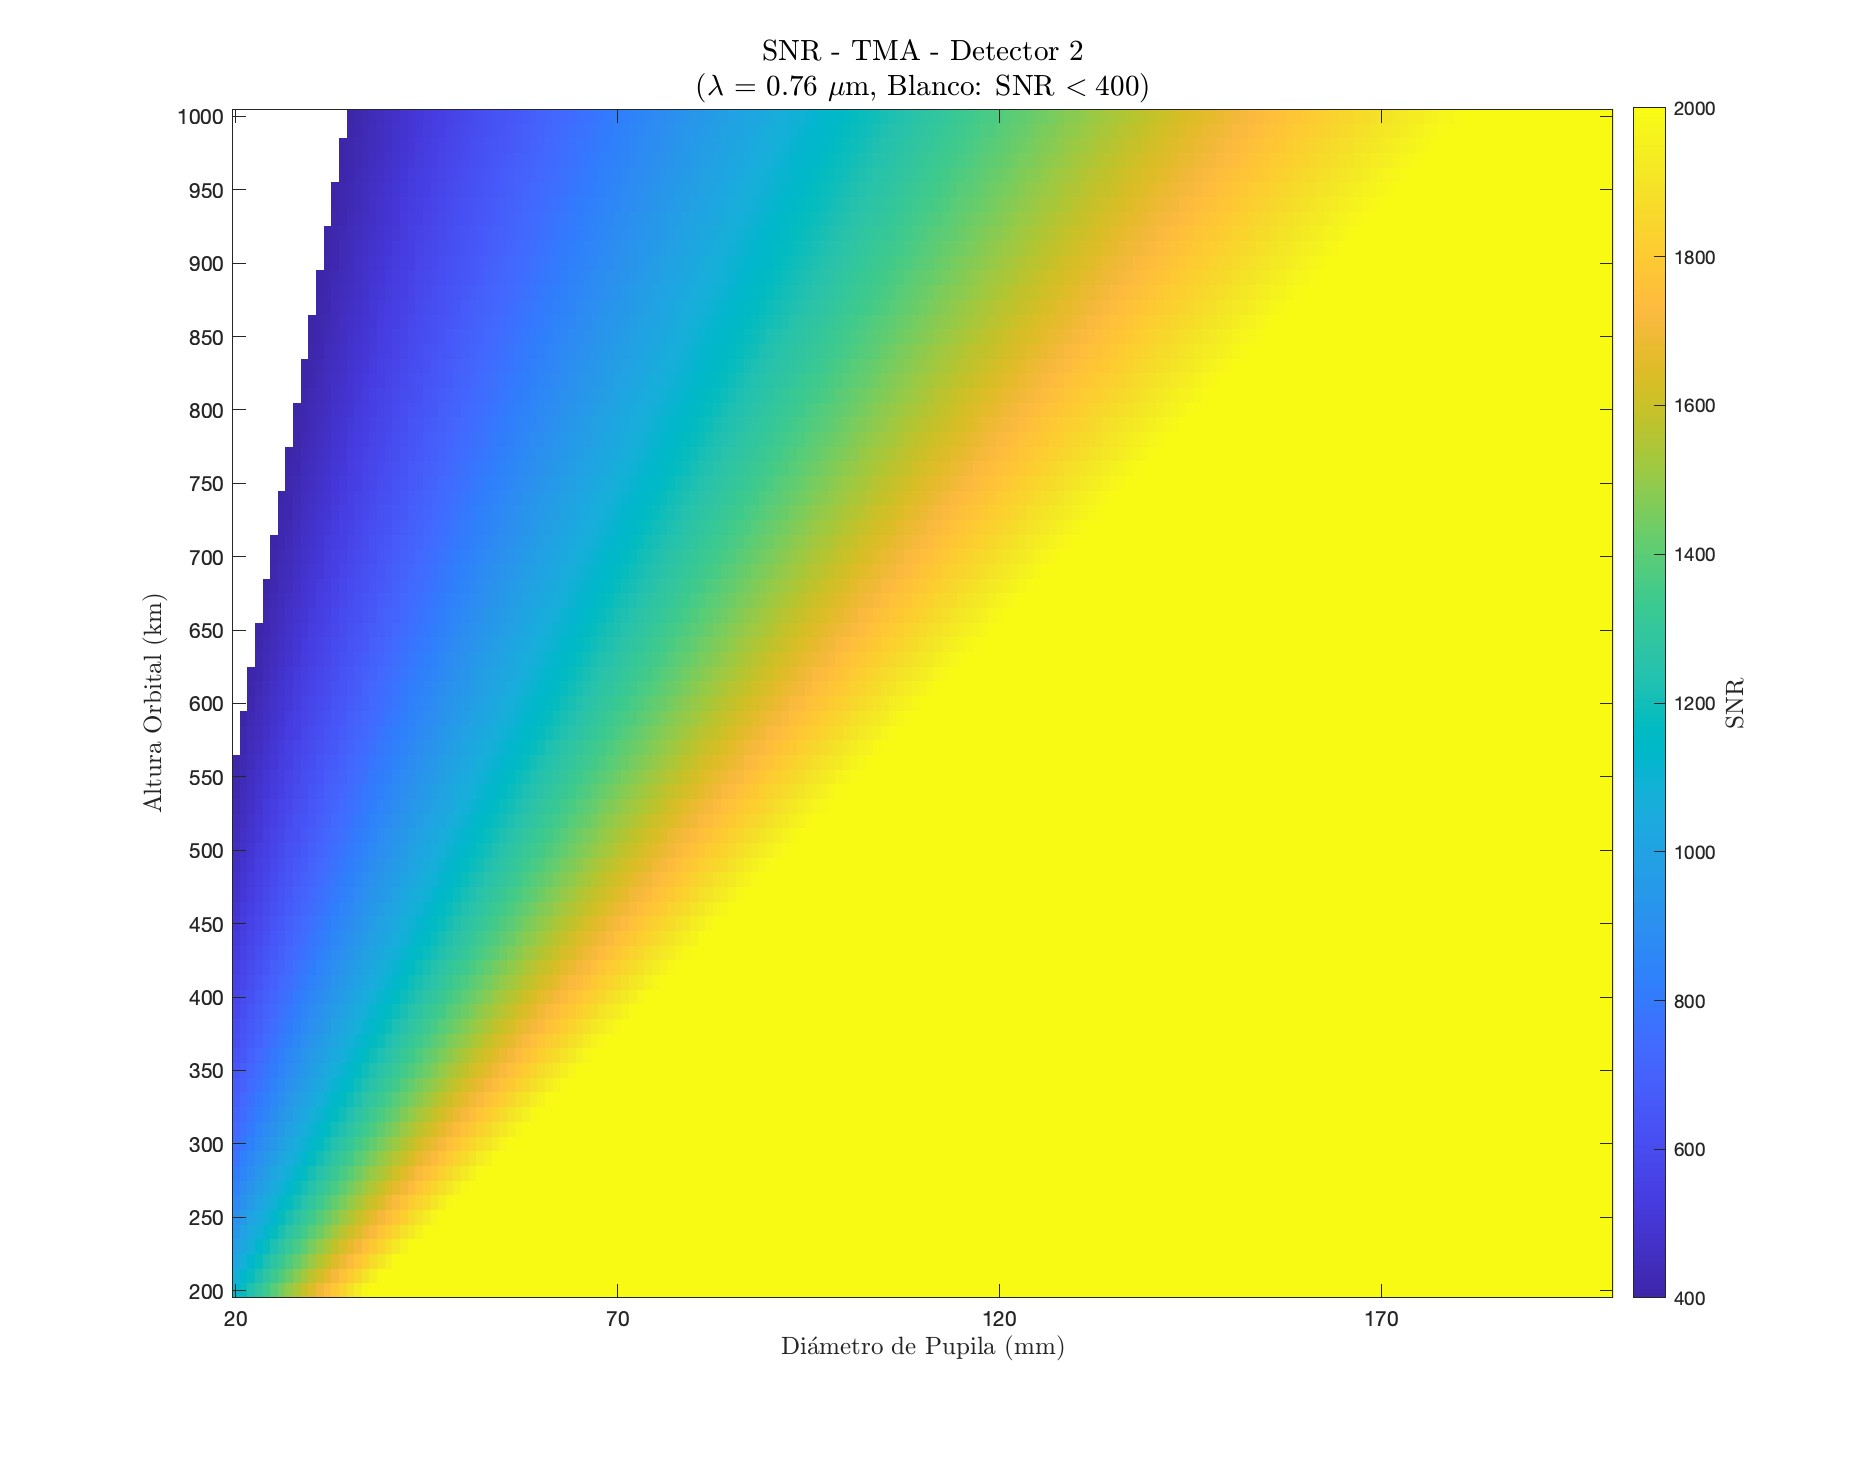
\includegraphics[width=0.48\linewidth]{4.Payload/SNR/SNR_Lambda3_Detector5_Telescopio4_heatmap.jpg} \\
\end{tabular}
% Nota: Reemplazar "0,76" con el valor de longitud de onda para Lambda 3.
\caption{Mapas de calor resultantes del calculo de SNR: Banda 0,76 \textmu m; Detector 5}
\end{figure}
\end{landscape}


%% DETECTOR 6
\begin{landscape}
\begin{figure}[p]
\centering
\setlength{\tabcolsep}{2pt}
\renewcommand{\arraystretch}{0}

\paragraph{Banda 0,76 \textmu m}
\begin{tabular}{cc}
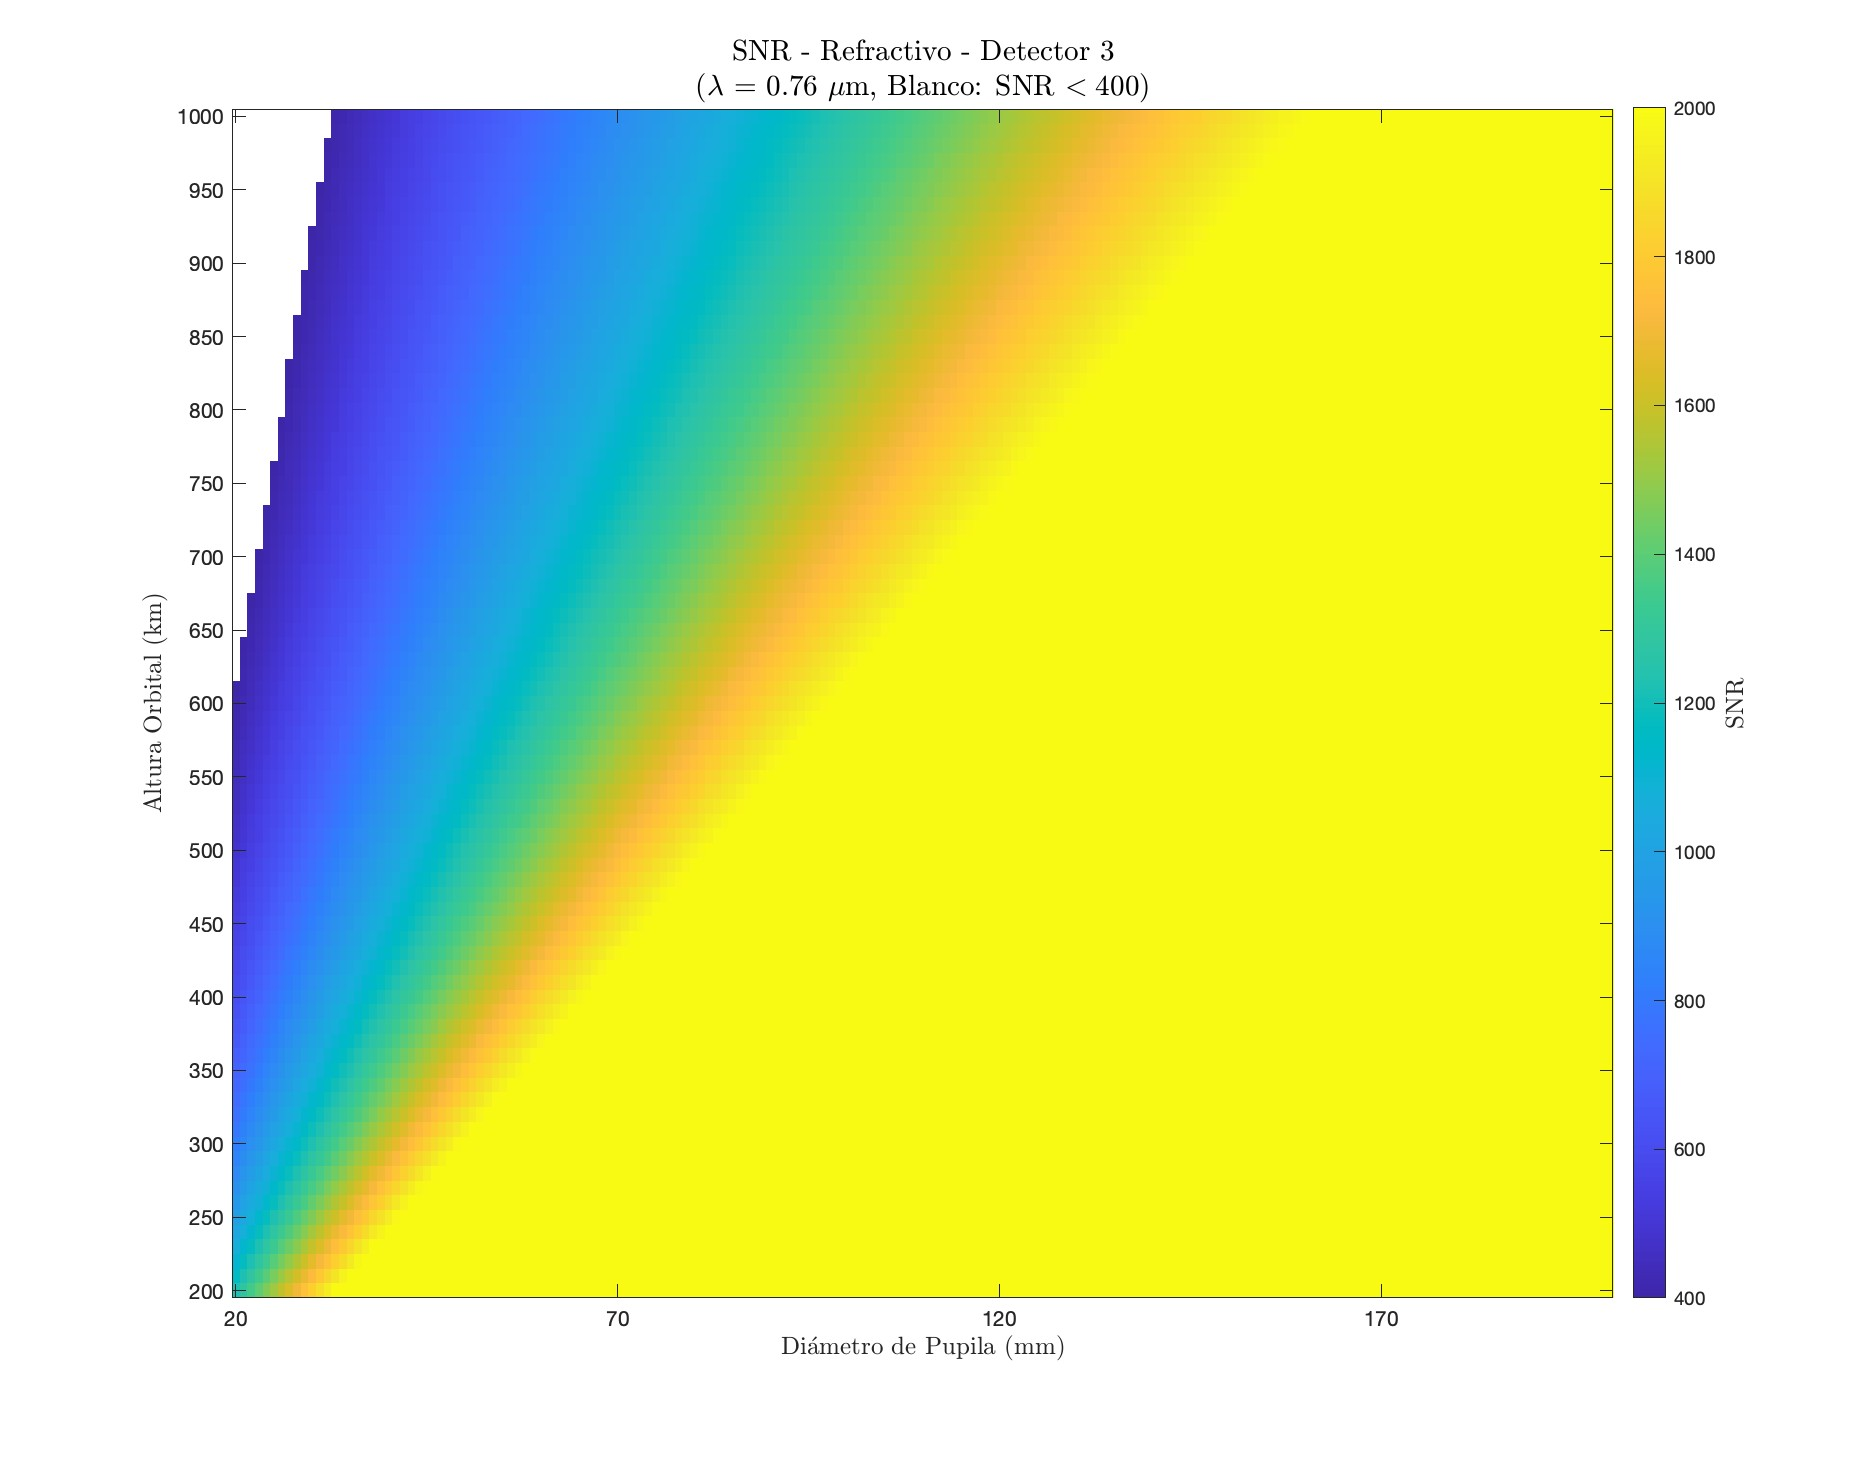
\includegraphics[width=0.48\linewidth]{4.Payload/SNR/SNR_Lambda3_Detector6_Telescopio1_heatmap.jpg} &
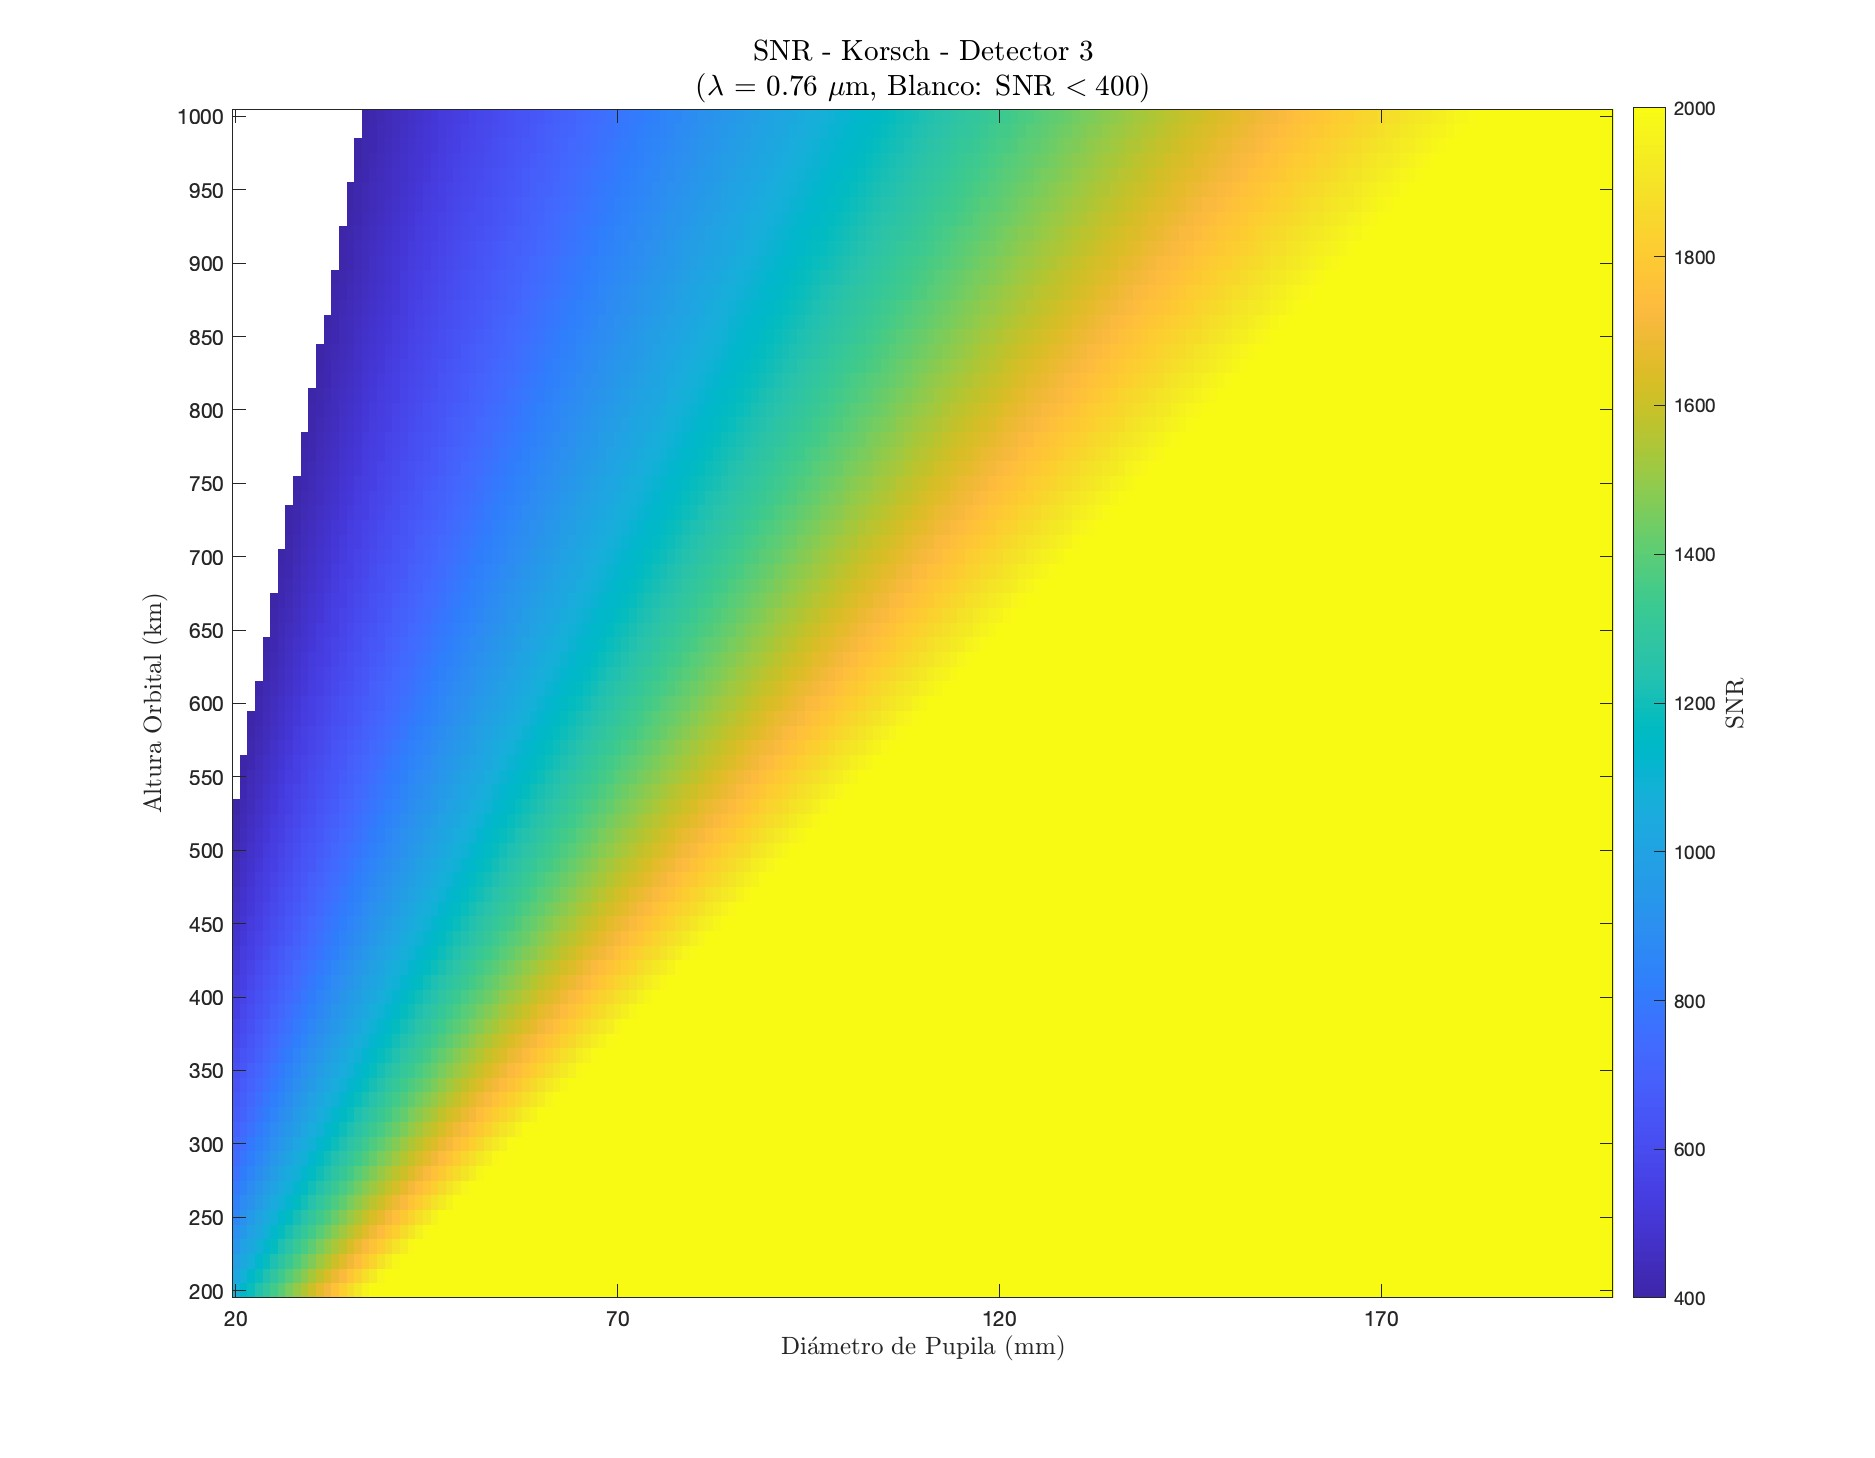
\includegraphics[width=0.48\linewidth]{4.Payload/SNR/SNR_Lambda3_Detector6_Telescopio2_heatmap.jpg} \\
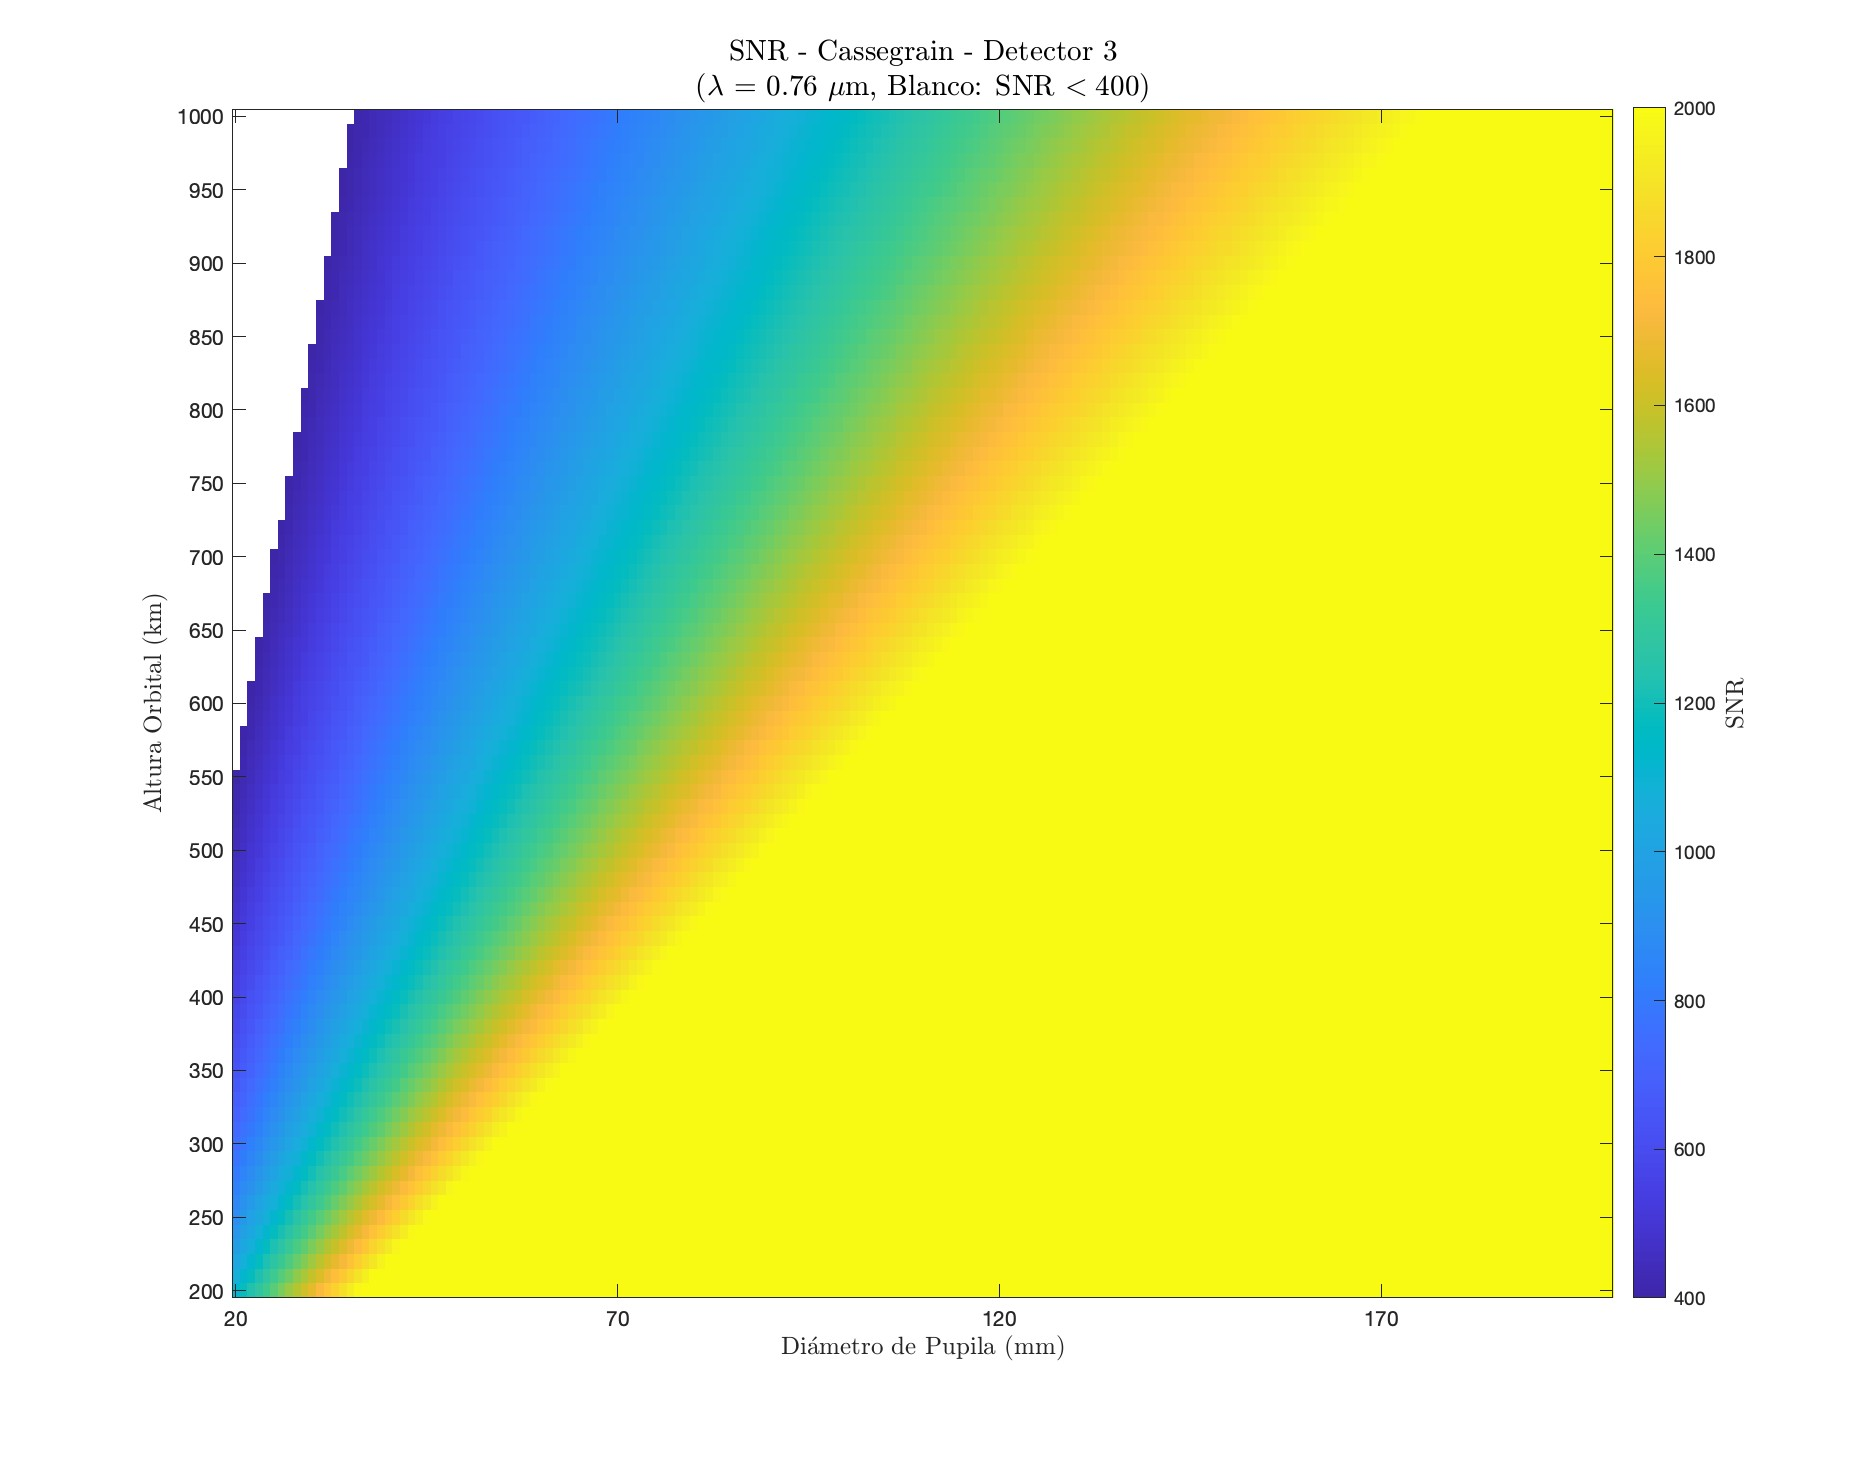
\includegraphics[width=0.48\linewidth]{4.Payload/SNR/SNR_Lambda3_Detector6_Telescopio3_heatmap.jpg} &
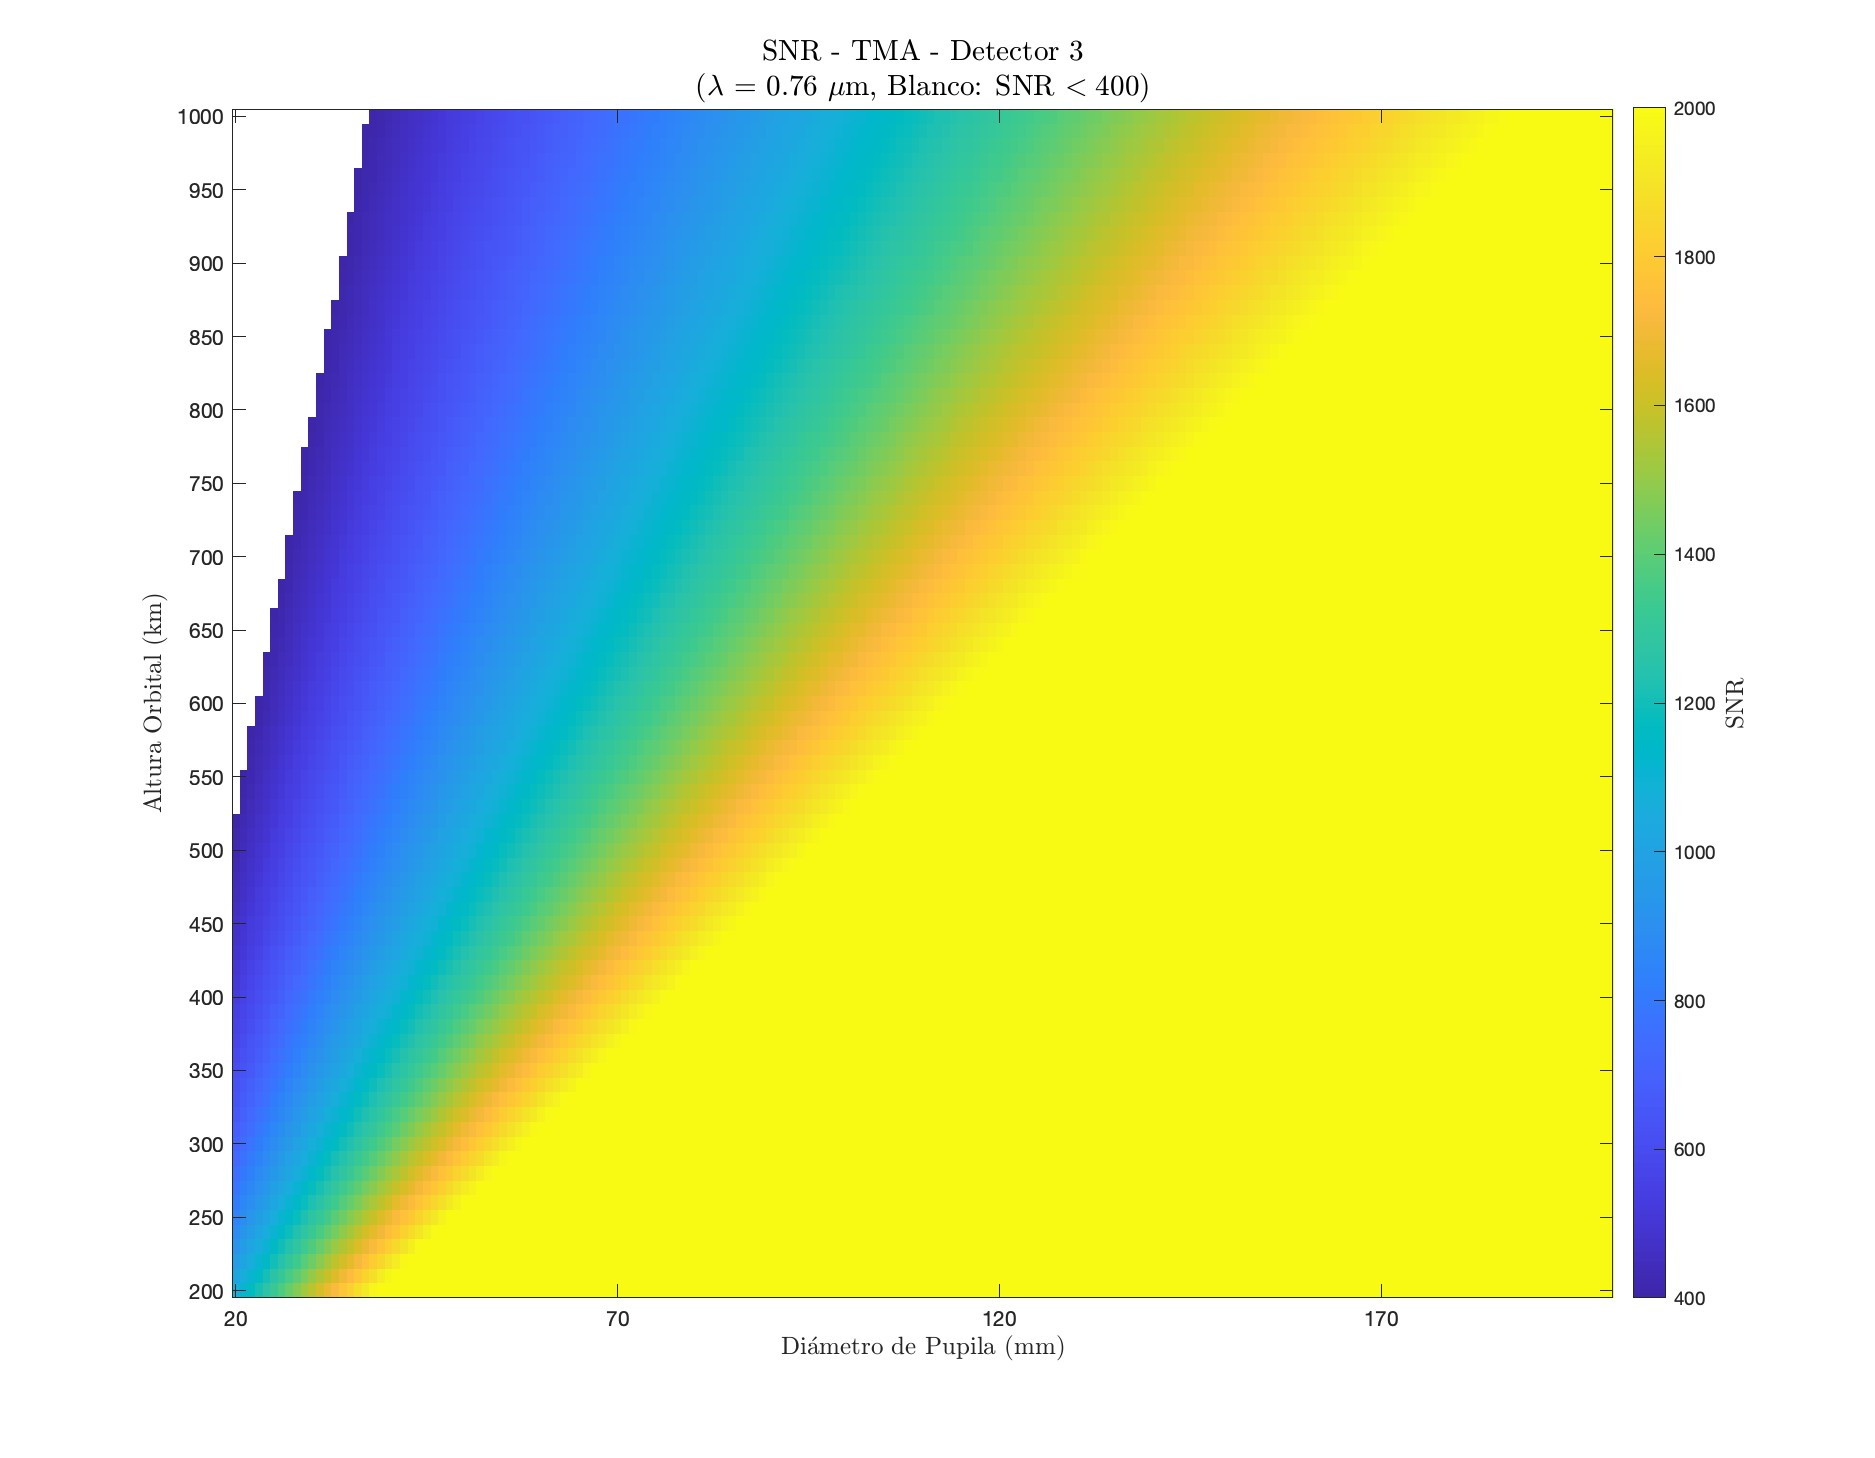
\includegraphics[width=0.48\linewidth]{4.Payload/SNR/SNR_Lambda3_Detector6_Telescopio4_heatmap.jpg} \\
\end{tabular}
% Nota: Reemplazar "0,76" con el valor de longitud de onda para Lambda 3.
\caption{Mapas de calor resultantes del calculo de SNR: Banda 0,76 \textmu m; Detector 6}
\end{figure}
\end{landscape}


%========================================================================================
%                                     LAMBDA 1
%========================================================================================
%% DETECTOR 1
\begin{landscape}
\begin{figure}[p]
\centering
\setlength{\tabcolsep}{2pt}
\renewcommand{\arraystretch}{0}

\paragraph{Banda 1,61 \textmu m}
\begin{tabular}{cc}
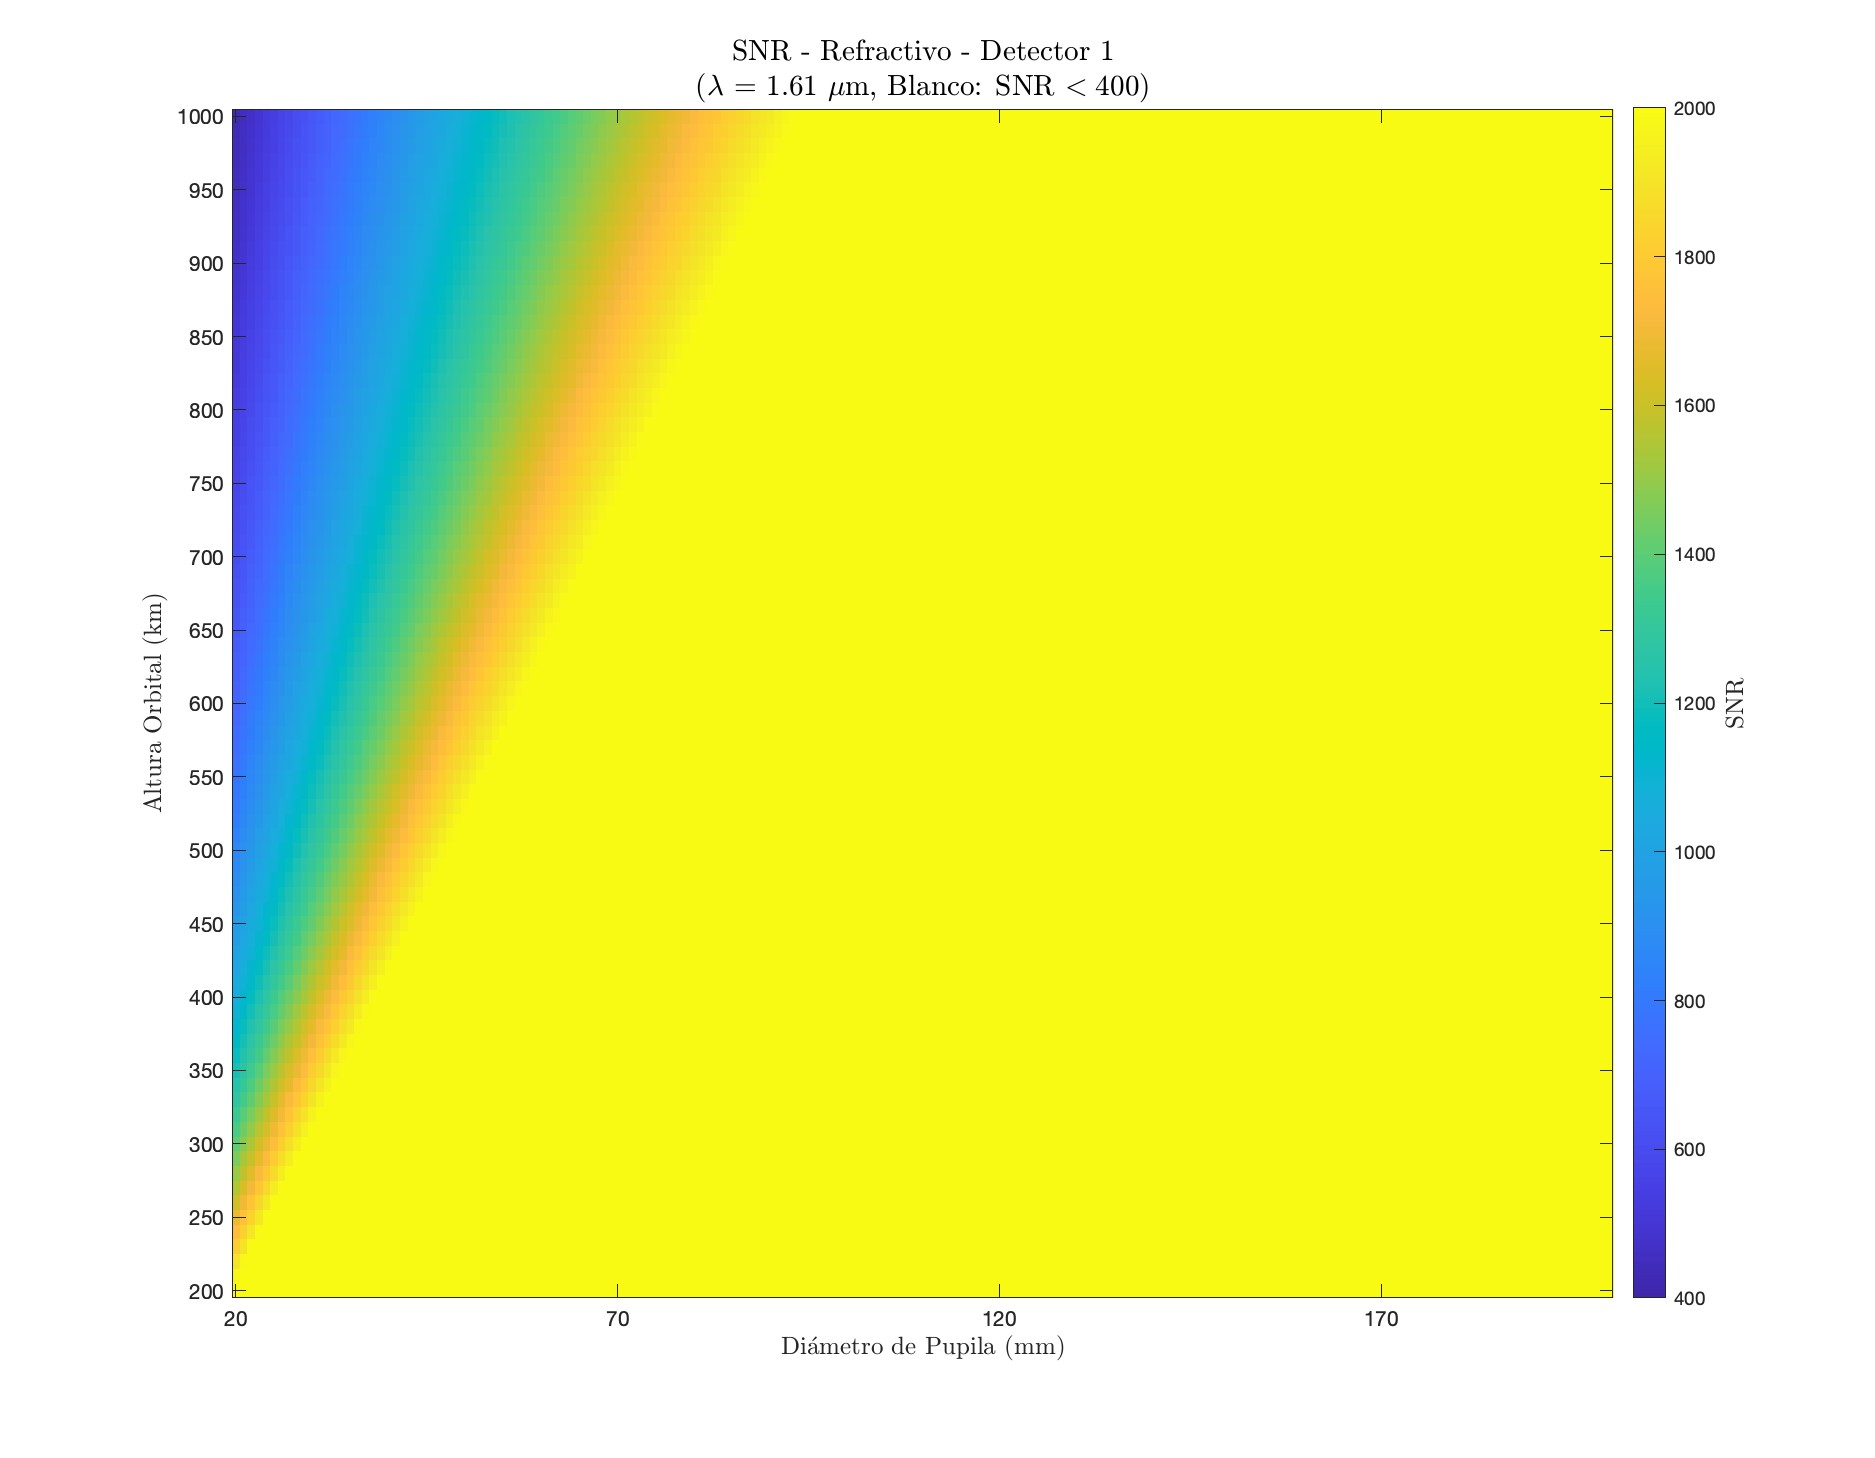
\includegraphics[width=0.48\linewidth]{4.Payload/SNR/SNR_Lambda1_Detector1_Telescopio1_heatmap.jpg} &
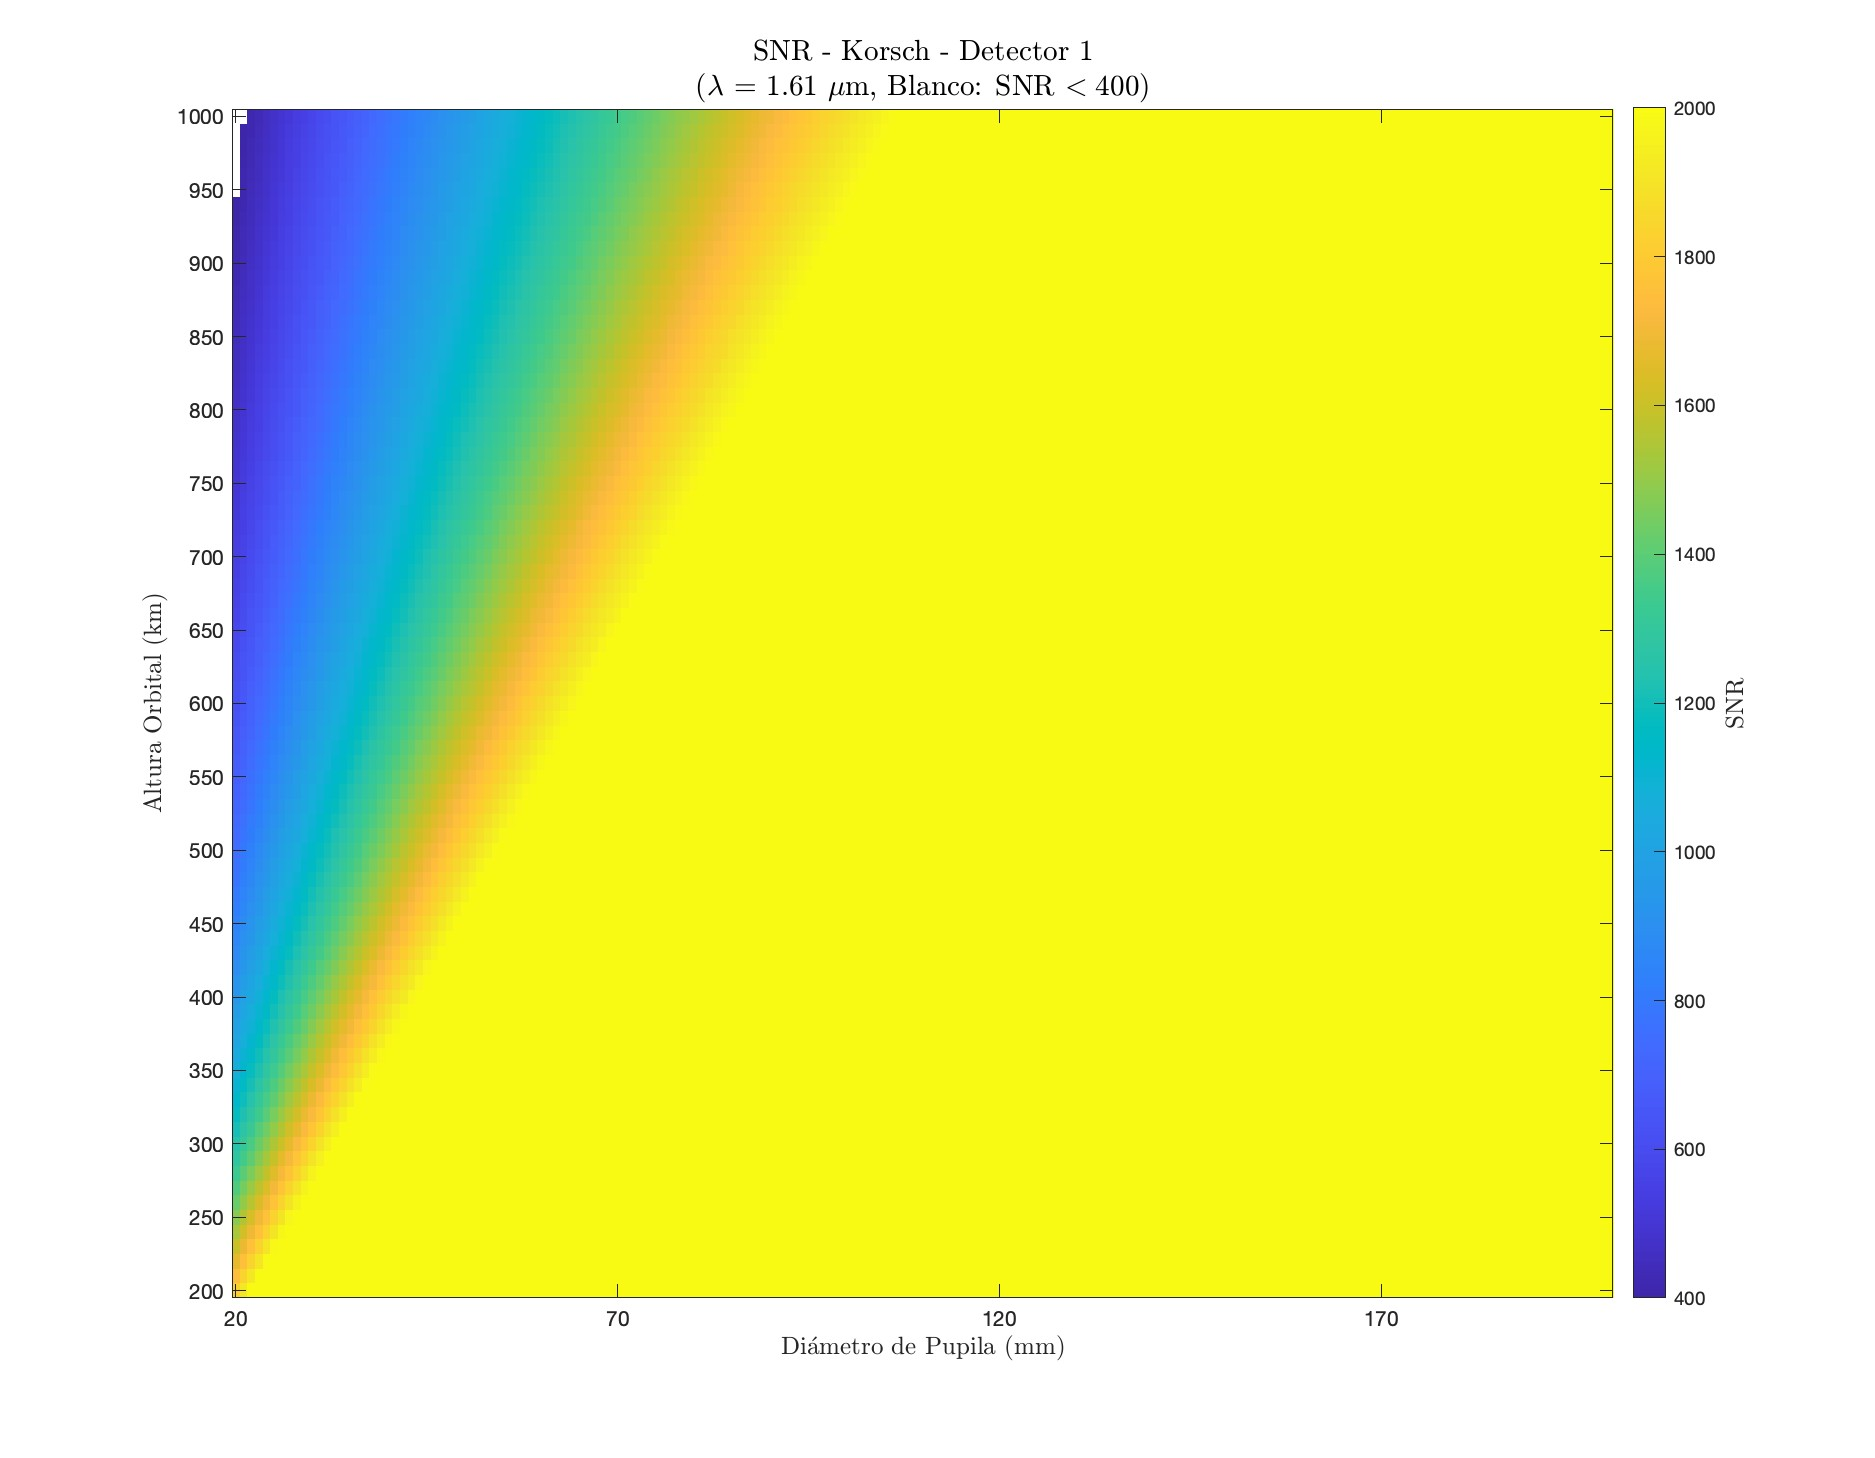
\includegraphics[width=0.48\linewidth]{4.Payload/SNR/SNR_Lambda1_Detector1_Telescopio2_heatmap.jpg} \\
\includegraphics[width=0.48\linewidth]{4.Payload/SNR/SNR_Lambda1_Detector1_Telescopio3_heatmap.jpg} &
\includegraphics[width=0.48\linewidth]{4.Payload/SNR/SNR_Lambda1_Detector1_Telescopio4_heatmap.jpg} \\
\end{tabular}
% Nota: Reemplazar "1,61" con el valor de longitud de onda para Lambda 1.
\caption{Mapas de calor resultantes del calculo de SNR: Banda 1,61 \textmu m; Detector 1}
\end{figure}
\end{landscape}


%% DETECTOR 2
\begin{landscape}
\begin{figure}[p]
\centering
\setlength{\tabcolsep}{2pt}
\renewcommand{\arraystretch}{0}

\paragraph{Banda 1,61 \textmu m}
\begin{tabular}{cc}
\includegraphics[width=0.48\linewidth]{4.Payload/SNR/SNR_Lambda1_Detector2_Telescopio1_heatmap.jpg} &
\includegraphics[width=0.48\linewidth]{4.Payload/SNR/SNR_Lambda1_Detector2_Telescopio2_heatmap.jpg} \\
\includegraphics[width=0.48\linewidth]{4.Payload/SNR/SNR_Lambda1_Detector2_Telescopio3_heatmap.jpg} &
\includegraphics[width=0.48\linewidth]{4.Payload/SNR/SNR_Lambda1_Detector2_Telescopio4_heatmap.jpg} \\
\end{tabular}
% Nota: Reemplazar "1,61" con el valor de longitud de onda para Lambda 1.
\caption{Mapas de calor resultantes del calculo de SNR: Banda 1,61 \textmu m; Detector 2}
\end{figure}
\end{landscape}


%% DETECTOR 3
\begin{landscape}
\begin{figure}[p]
\centering
\setlength{\tabcolsep}{2pt}
\renewcommand{\arraystretch}{0}

\paragraph{Banda 1,61 \textmu m}
\begin{tabular}{cc}
\includegraphics[width=0.48\linewidth]{4.Payload/SNR/SNR_Lambda1_Detector3_Telescopio1_heatmap.jpg} &
\includegraphics[width=0.48\linewidth]{4.Payload/SNR/SNR_Lambda1_Detector3_Telescopio2_heatmap.jpg} \\
\includegraphics[width=0.48\linewidth]{4.Payload/SNR/SNR_Lambda1_Detector3_Telescopio3_heatmap.jpg} &
\includegraphics[width=0.48\linewidth]{4.Payload/SNR/SNR_Lambda1_Detector3_Telescopio4_heatmap.jpg} \\
\end{tabular}
% Nota: Reemplazar "1,61" con el valor de longitud de onda para Lambda 1.
\caption{Mapas de calor resultantes del calculo de SNR: Banda 1,61 \textmu m; Detector 3}
\end{figure}
\end{landscape}


%========================================================================================
%                                     LAMBDA 2
%========================================================================================
%% DETECTOR 1
\begin{landscape}
\begin{figure}[p]
\centering
\setlength{\tabcolsep}{2pt}
\renewcommand{\arraystretch}{0}

\paragraph{Banda 2,01 \textmu m}
\begin{tabular}{cc}
\includegraphics[width=0.48\linewidth]{4.Payload/SNR/SNR_Lambda2_Detector1_Telescopio1_heatmap.jpg} &
\includegraphics[width=0.48\linewidth]{4.Payload/SNR/SNR_Lambda2_Detector1_Telescopio2_heatmap.jpg} \\
\includegraphics[width=0.48\linewidth]{4.Payload/SNR/SNR_Lambda2_Detector1_Telescopio3_heatmap.jpg} &
\includegraphics[width=0.48\linewidth]{4.Payload/SNR/SNR_Lambda2_Detector1_Telescopio4_heatmap.jpg} \\
\end{tabular}
\caption{Mapas de calor resultantes del calculo de SNR: Banda 2,01 \textmu m; Detector 1}
\end{figure}
\end{landscape}


%% DETECTOR 2
\begin{landscape}
\begin{figure}[p]
\centering
\setlength{\tabcolsep}{2pt}
\renewcommand{\arraystretch}{0}

\paragraph{Banda 2,01 \textmu m}
\begin{tabular}{cc}
\includegraphics[width=0.48\linewidth]{4.Payload/SNR/SNR_Lambda2_Detector2_Telescopio1_heatmap.jpg} &
\includegraphics[width=0.48\linewidth]{4.Payload/SNR/SNR_Lambda2_Detector2_Telescopio2_heatmap.jpg} \\
\includegraphics[width=0.48\linewidth]{4.Payload/SNR/SNR_Lambda2_Detector2_Telescopio3_heatmap.jpg} &
\includegraphics[width=0.48\linewidth]{4.Payload/SNR/SNR_Lambda2_Detector2_Telescopio4_heatmap.jpg} \\
\end{tabular}
\caption{Mapas de calor resultantes del calculo de SNR: Banda 2,01 \textmu m; Detector 2}
\end{figure}
\end{landscape}


%% DETECTOR 3
\begin{landscape}
\begin{figure}[p]
\centering
\setlength{\tabcolsep}{2pt}
\renewcommand{\arraystretch}{0}

\paragraph{Banda 2,01 \textmu m}
\begin{tabular}{cc}
\includegraphics[width=0.48\linewidth]{4.Payload/SNR/SNR_Lambda2_Detector3_Telescopio1_heatmap.jpg} &
\includegraphics[width=0.48\linewidth]{4.Payload/SNR/SNR_Lambda2_Detector3_Telescopio2_heatmap.jpg} \\
\includegraphics[width=0.48\linewidth]{4.Payload/SNR/SNR_Lambda2_Detector3_Telescopio3_heatmap.jpg} &
\includegraphics[width=0.48\linewidth]{4.Payload/SNR/SNR_Lambda2_Detector3_Telescopio4_heatmap.jpg} \\
\end{tabular}
\caption{Mapas de calor resultantes del calculo de SNR: Banda 2,01 \textmu m; Detector 3}
\end{figure}
\end{landscape}














\newpage
\subsubsection{Análisis de Configuraciones. Posibles soluciones}
\addcontentsline{toc}{section}{Análisis de Configuraciones. Posibles soluciones}
\VerbatimInput{zzAnnex/TablasAnnex/configanalysis}
\newpage

\subsubsection{Resultado de simulación de impulsos necesarios}
\addcontentsline{toc}{section}{Resultado de simulación de impulsos necesarios}
\VerbatimInput{zzAnnex/TablasAnnex/burnssim}